\documentclass{FastFyp}
\begin{document}
\raggedbottom
\newcommand{\supervisor}{Dr. Ammar Haider \\ Co-Supervisor: Ms. Nosheen Manzoor}
\newcommand{\university}{National University of Computer and Emerging Sciences, Lahore}
\newcommand{\fyptitle}{PhishHook: Lightweight Client-Side Phishing Detection using Hybrid Approach}
\newcommand{\degree}{BS}
\newcommand{\Studentone}{Abdullah Shahbaz     23L-0874    BS(CS)}
\newcommand{\Studenttwo}{Muhammad Hassan Raza     23L-3049    BS(CS)}
\newcommand{\Studentthree}{Muhammad Ibrahim     23L-0837    BS(CS)}
\date{\today}
\renewcommand{\contentsname}{Table of Contents}
\newcommand{\defitem}[2]{\noindent\textbf{#1}: #2\par}
\makeatletter
    \begin{titlepage}
        
\includegraphics[width=0.2\linewidth]{Figures/nulogo.png}\hfill
        
\includegraphics[width=0.2\linewidth]{Figures/fast.png}\\
        \begin{center}
            {\large\bfseries \university}\\[7ex]
            
\includegraphics[width=0.4\linewidth]{Figures/fastlogo.png}\\[8ex]
            {\huge \bfseries  \fyptitle }\\[10ex]
            {\Studentone}\\{\Studenttwo}\\{\Studentthree}\\[4ex]
            {Supervisor: \supervisor} \\ [10ex]
            {Final Year Project}\\
            {\large \@date}
        \end{center}
    \end{titlepage}
\makeatother
\frontmatter

\newpage \thispagestyle{empty} \mbox{} \newpage

\pagestyle{empty}


\newcommand{\signatureline}[1]{%
    \parbox[t]{6cm}{\raggedleft
        \includegraphics[height=1.8cm]{#1}\\[-0.3cm]
        \makebox[6cm]{\dotfill}%
    }%
}

\section*{\begin{center}{Anti-Plagiarism Declaration} \end{center}}
This is to declare that the above publication was produced under the:
\begin{flushleft}
\bf Title: \fyptitle
\end{flushleft}

is the sole contribution of the author(s), and no part hereof has been reproduced as it is the basis (cut and paste) that can be considered Plagiarism. All referenced parts have been used to argue the idea and cited properly. I/We will be responsible and liable for any consequence if a violation of this declaration is determined.
\\[4ex]
Date: \today
\begin{flushright}
	\begin{tabular}{rl}
		\multicolumn{2}{r}{Name: Abdullah Shahbaz} \\[0.2cm]
		Signature: & \makebox[5cm]{\centering \raisebox{-0.2cm}{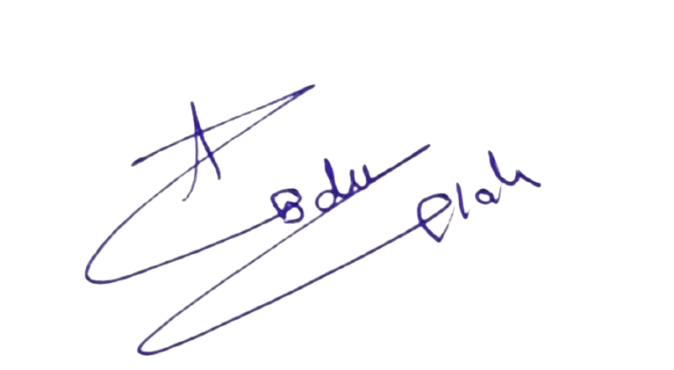
\includegraphics[height=1.3cm]{Figures/signature_abdullah.png}}} \\[-0.6cm]
		& \makebox[5cm]{\dotfill} \\[0.8cm]
		
		\multicolumn{2}{r}{Name: Muhammad Hassan Raza} \\[0.2cm]
		Signature: & \makebox[5cm]{\centering \raisebox{-0.2cm}{
\includegraphics[height=1.6cm]{Figures/signature_hassan.png}}} \\[-0.6cm]
		& \makebox[5cm]{\dotfill} \\[0.8cm]
		
		\multicolumn{2}{r}{Name: Muhammad Ibrahim} \\[0.2cm]
		Signature: & \makebox[5cm]{\centering \raisebox{-0.2cm}{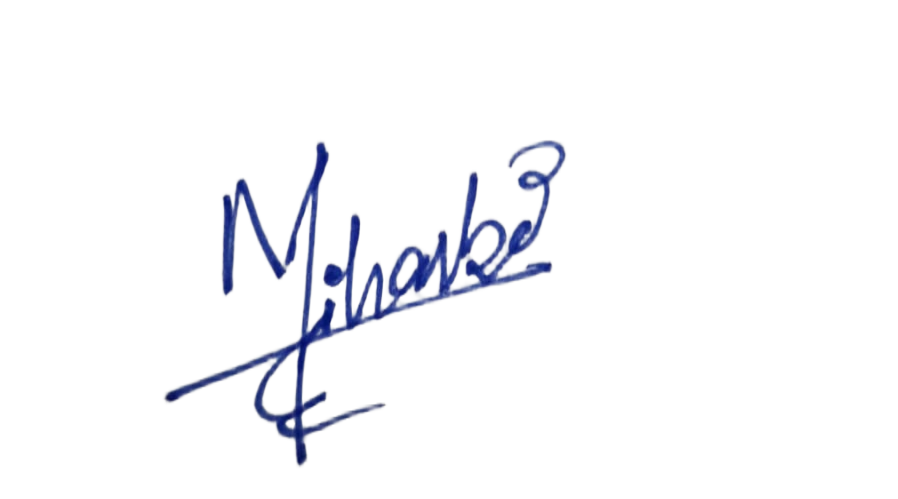
\includegraphics[width=4.5cm]{Figures/signature_ibrahim.png}}} \\[-0.6cm]
		& \makebox[5cm]{\dotfill}
	\end{tabular}
\end{flushright}

\vspace{0.5cm} % Reduces the gap before the horizontal line

\vspace{0.5cm}
\hrule
\vspace{0.5cm}

\section*{Author's Declaration}
This states Authors' declaration that the work presented in the report is their own, and has not been submitted/presented previously to any other institution or organization.
\pagebreak

\section*{Abstract}
Phishing is still a prevalent threat and many detection solutions are based on cloud services, external reputation checks or are resource heavy. These reasons can raise user privacy and overall performance issues. This project contains a phishing detection extension for Chromium browsers that is lightweight and based on Manifest V3. Runs All Analysis locally based on the URL and already rendered page content, without any network lookups or data being sent anywhere outside the device.

PhishHook is a combination of two modules for web page detection. The unsupervised URL model requires no labelled phishing samples to determine an anomaly score, but it is trained using only benign URLs. The second module applies a quantised MobileBERT classifier to the DOM-based text and text that is visible on the screen to estimate the probability of phishing. Using a logistic-regression model, the percentile-ranked URL score is combined with a calibrated DOM score to create a risk score.

When it comes to email detection, a fine-tuned MobileBERT teacher is transferred with knowledge to a compact BiLSTM student by knowledge distillation. The student model is deployed and the content displayed in the webmail interface is analysed.The study compares the URL module performance with a supervised reference based URL module performance, measures the accuracy and robustness of the quantised DOM module and explores whether the combination of both modules minimizes false alarms.

\vspace{0.5em}



\pagebreak

\section*{Executive Summary}
The reason phishing continues to work is that it can be easily set up by an attacker within hours, before a blocklist can be aware of it. Cloud detectors can catch more but they must see what the user is browsing, and many of the deep models are too heavy to be carried by the browser. PhishHook is a Chromium Manifest V3 extension that is only active in the URL and from the page the user has opened. Does not make any of the network calls and does not send anything off the device.

Chapter 1 presents the problem, our three research questions, and the paper that we build on a DOM input without the URL, an unsupervised URL module, monitoring after the page loads and a distilled email detector. The vision is presented in Chapter 2. There is no light weight, private and accurate client side detector for both web and email phishing, and previous work generally evaluates on balanced data, which camouflages the number of false alarms a real user would encounter. The following results are therefore reported based on the assumption of the following phishing rates: 1 in 100, 1 in 1,000 and 1 in 10,000. This chapter identifies our objectives, isolates the cloud from cloud inference, eliminates the need for WHOIS or DNS lookups, eliminates server components.

Chapter 3 reviews 22 papers in five groups: unsupervised URL detection, supervised web detection, hybrid methods, email detection with distillation, and client-side deployment. Many of them depend on cloud services or external metadata, are tested only on balanced benchmarks, or never check unseen sources and later time periods. Very few measure what the model costs inside a browser. These gaps shaped our choices. The extension is required to perform a set of operations as described in Chapter 4. Reads URL and DOM locally, scores each, aggregates scores and continues to monitor a page after it is loaded, shows warning to user to dismiss. Five use cases, the interface and a risk analysis follow.

Chapter 5 explains the method. It names the five datasets (PhishPedia, PhishTank, Tranco, PhiUSIIL and MeAJOR) and the rules that keep training, calibration and test data apart. The URL module compares an autoencoder, an Isolation Forest and a K-Means baseline, all trained on benign URLs only. The DOM module is a quantised MobileBERT, compared against LightGBM. A small logistic regression combines the two scores, and for email a MobileBERT teacher is distilled into a BiLSTM student.

Chapter 6 turns the method into a design. The extension has a content script that reads the URL and rendered DOM, a service worker that coordinates the work, an offscreen document that runs the ONNX models in WebAssembly, and a popup. Chrome stops an idle service worker after about 30 seconds, so the models run in the offscreen document. Manifest V3 cannot block a page before it opens, so checks happen after load, on DOM changes and at form submission. The system is split into five subsystems: extraction, detection and fusion, email, monitoring and warnings, and email-to-web correlation. Nothing is written to disk, and every model ships inside the extension package.

Chapter 7 describes the code written so far: nine modules in three Python pipelines, run on Colab and Kaggle. We defined 27 checks, ran 26, and 22 passed. Four failed. One ablation input is empty for many phishing pages, two URL thresholds were set on test data, and the URL scheme was used as a feature although the design leaves it out. The extension itself is still a prototype. The results of experiments are presented in Chapter 9. All the experiments which were performed and their results and comparisons are present in this chapter. 

Chapter 10 closes with what FYP-1 achieved and what remains. In FYP-2 we will finish the distillation run, build one test set for the fused system, fix the URL defects and re-run those experiments, connect the models to the extension, complete the extension work so it is ready to deploy in real world and then measure latency, memory and CPU use and run a small user study of the warnings.

To conclude, PhishHook aims to advance the state of lightweight, privacy-preserving phishing detection by combining an unsupervised URL module, a supervised DOM classifier, a fusion meta-classifier, dynamic post-load monitoring, and a distilled email detector, all running entirely on the user's device. The project is designed to be reproducible, honest about its limitations, and practical to deploy in a standard Chromium browser.
\pagebreak

\pagestyle{fancy}
\tableofcontents

\pagebreak
\listoffigures
\addcontentsline{toc}{chapter}{List of Figures}
\pagebreak
\listoftables
\addcontentsline{toc}{chapter}{List of Tables}

\mainmatter

% ============================================================
% CHAPTER 1: INTRODUCTION
% ============================================================
\chapter{Introduction}
\label{ch:intro}
Phishing is still one of the most prolific and adaptive threats in cybersecurity. Traditional defenses are being foiled by attackers because they use dynamic webpage behavior, post-load DOM manipulation and AI-generated email content. Only known threats will be caught by blocklists and cloud-based detection will have latency, user privacy and connection dependency problems. PhishHook addresses these limitations by performing phishing detection entirely on the user's device, inside a Chromium Manifest V3 extension, using only the URL string and the already-rendered DOM of the page the user has loaded. All of the working is done in Chrome and data never leave the user device. 

PhishHook uses a dual framework web pipeline. A lightweight unsupervised model analyses the URL string and assigns an anomaly score, on the premise that phishing URLs deviate from patterns learned from benign URLs only. In parallel, a supervised quantised MobileBERT model analyses DOM-derived text (title, form fields and labels, link domains, and visible text) and produces a calibrated phishing probability. A small L2-regularised logistic regression meta-classifier fuses the two scores into a single risk assessment. For email, a MobileBERT teacher is fine-tuned offline and distilled into a compact BiLSTM student only the student is deployed, and it consumes only what is visible in the webmail DOM. This report provide details of the design, implementation and evaluation of this pipeline,
It includes the entirely-local input design, the unsupervised URL anomaly module, the supervised DOM module, the fusion method, the distillation methodology for email and its analysis for the MV3 deployment.


\section{Purpose of this Document}
The purpose of this document is to present the design, implementation, and evaluation of our FYP, PhishHook which addresses the growing problem of phishing attacks that bypass traditional blocklists and cloud-based detectors. Nowadays, phishing pages can be created, and edited in a matter of hours and cloud based detection methods create privacy and network dependency issues. Old and privacy-compromising detection strategies put customers at risk of credential theft and financial fraud. Legacy and privacy-compromising detection strategies put customers at risk of credential theft and financial fraud. Our project uses a dual framework approach for this challenge as a client-side solution that can be integrated directly into a Chromium Manifest V3 browser extension to detect anomalies in URLs using unsupervised learning, classify the DOM using supervised learning and knowledge distillation without any data being sent off-device.

The research questions we aim to explore are: (RQ1) How well does an unsupervised URL anomaly model, trained on benign URLs only, detect phishing URLs at realistic base rates, and how does it compare with a supervised URL baseline used only as a reference? (RQ2) Which parts of the URL and DOM input contribute most to detection, and what is the accuracy versus resource trade-off inside the browser? (RQ3) Does a quantised MobileBERT model perform better than a LightGBM model trained on engineered features when detecting phishing attacks using the same information extracted from the rendered DOM?

In this effort, we hope to improve the state of the art in lightweight, privacy-preserving phishing detection, and to offer a practical, reproducible phishing detection system that can be extended by future researchers and browser extension developers. This report describes the methodology, design, implementation, testing and evaluation of PhishHook, also the limitations, threat model and future work.


\section{Contributions over PhishLang}
\label{sec:contributions}
PhishHook builds on the work of PhishLang \cite{phishlang2026}, which demonstrated that phishing detection can be performed entirely on the client side using MobileBERT over actionable HTML elements. In the following subsections, the concrete contributions of PhishHook towards PhishLang are explained. These changes address several practical gaps we found when testing the original architecture. 

\subsection{URL-Excluded DOM Input}
The page URL is kept separate from the supervised DOM model. This allows the URL and DOM modules to work independently and complement each other. It also makes it possible to properly evaluate the contribution of each input through the ablation study (RQ2). PhishLang offers actionable HTML elements, but does not mandate this separation.

\subsection{Unsupervised URL Anomaly Module}
PhishHook also introduces a second training path that uses unsupervised learning to analyse URL strings without relying on labelled phishing data. A predefined selection rule is then used to decide which model will be deployed. PhishLang is a single supervised model. By keeping a fully unsupervised detector in the pipeline, PhishHook does not depend entirely on the quality or freshness of the labelled training data.

\subsection{Dynamic Monitoring}
PhishHook continuously monitors the rendered DOM for security-relevant changes after page load, such as new forms appearing, form destinations being modified, or significant script changes. This addresses a documented limitation of PhishLang, which performs static analysis of page source code at the moment of access but does not observe post-load DOM mutations or dynamically injected phishing elements.

\subsection{Distilled Email Detector}
PhishHook adds a separate email pipeline using knowledge distillation from an offline MobileBERT teacher into a deployed BiLSTM student. PhishLang does not address email. This is treated as a stretch goal in the project scope.

\section{Intended Audience}
This document is intended for the following readers:
\begin{itemize}
    \item Academic Panel and Supervisors, to find out the adequacy of the research and research design
    methodology and breakthrough of the proposed system.

    \item End users, such as general internet users, students, and professionals, who want to understand what PhishHook does, what it protects them from, and how their privacy is preserved because no data leaves their device.
\end{itemize}


\section{Definitions, Acronyms, and Abbreviations}
\label{sec:definitions}
This section lists the abbreviations and technical terms used in this report so that later chapters can use them without repeating their meaning. Abbreviations come first, followed by the terms that describe the PhishHook modules and the evaluation setup.

\vspace{0.5em}
\noindent\textbf{BiLSTM:} Bidirectional Long Short-Term Memory\par\medskip
\noindent\textbf{DOM:} Document Object Model\par\medskip
\noindent\textbf{FPR:} False Positive Rate\par\medskip
\noindent\textbf{FYP:} Final Year Project\par\medskip
\noindent\textbf{MV3:} Manifest V3, the current extension platform for Chromium-based browsers\par\medskip
\noindent\textbf{ONNX:} Open Neural Network Exchange\par\medskip
\noindent\textbf{PR-AUC:} Area Under the Precision--Recall Curve\par\medskip
\noindent\textbf{RQ:} Research Question\par\medskip
\noindent\textbf{SDG:} Sustainable Development Goal\par\medskip
\noindent\textbf{TPR:} True Positive Rate\par\medskip

\noindent\textbf{PhishHook:} The lightweight, client-side phishing detection framework proposed in this report\par\medskip
\noindent\textbf{Unsupervised URL Module:} The component that detects suspicious URLs without using any labelled training data\par\medskip
\noindent\textbf{Character-Level Autoencoder:} A neural network that learns to rebuild benign URLs one character at a time, so a high reconstruction error per character points to an abnormal URL\par\medskip
\noindent\textbf{Isolation Forest:} An ensemble anomaly detection method that separates observations through random splits, applied here to the engineered lexical URL features\par\medskip
\noindent\textbf{Anomaly Score:} The value that the unsupervised model outputs for a given URL\par\medskip
\noindent\textbf{Engineered Lexical Features:} Hand-crafted statistics calculated separately for the host, path, and query of a URL, such as its length, digit ratio, Shannon entropy, subdomain depth, and the presence of punycode or percent-encoding\par\medskip
\noindent\textbf{Supervised DOM Module:} The component trained on a labelled dataset that detects phishing from the DOM of a page\par\medskip
\noindent\textbf{MobileBERT:} A compact language model used as the supervised DOM classifier and as the teacher for the email model\par\medskip
\noindent\textbf{Fusion Meta-Classifier:} A model that combines the URL score from the unsupervised module and the DOM score from the supervised module into a single decision\par\medskip
\noindent\textbf{Temperature Calibration:} A post-hoc adjustment of model logits so that predicted probabilities better match true likelihoods, fitted on the quantised DOM model because quantisation changes the logits\par\medskip
\noindent\textbf{Percentile Rank Transformation:} The conversion of a raw anomaly score into its percentile within a fixed set of benign validation scores from the quantised URL model, which places the URL and DOM inputs of the fusion stage on comparable scales\par\medskip
\noindent\textbf{Knowledge Distillation:} A training technique in which a large teacher model passes its learned behaviour to a smaller student model\par\medskip
\noindent\textbf{Teacher Model:} The fine-tuned MobileBERT used offline to generate soft labels for the email student\par\medskip
\noindent\textbf{Student Model:} The distilled BiLSTM that is exported and deployed for email phishing detection\par\medskip
\noindent\textbf{Soft Labels:} The probability distributions produced by the teacher and used to train the student\par\medskip
\noindent\textbf{Temperature (T):} A scaling value applied to the teacher logits to soften the soft-label distribution during distillation\par\medskip
\noindent\textbf{Quantisation:} Reducing the numerical precision of model weights (for example fp32, fp16, or int8) to shrink the model and lower latency\par\medskip
\noindent\textbf{Temporal Split:} A division of the data by time, so the training set contains only samples older than those in the test set\par\medskip
\noindent\textbf{Source-Disjoint Split:} A division of the data in which the test samples come from different sources than the training samples\par\medskip
\noindent\textbf{Popularity Bias:} The tendency to wrongly flag a benign URL from a low-ranked website, usually one with a long path\par\medskip


\section{Conclusion}
To conclude, this chapter has been the introduction to the important problem of phishing attacks which can bypass the traditional blocklists and cloud detectors, and presented some of the design considerations of PhishHook. Modern day threat vectors require detection methods that are accurate, efficient and privacy preserving but most current methods either use cloud service or use outdated blocklists or do not take into account the behavior of modern day phishing websites after loading. The gap in the field was attempted to be bridged in our approach using a hybrid system utilizing unsupervised URL anomaly detector, supervised DOM classification, continuous post-load DOM behavior analysis and a email detector distilled for use on the user's device without any transfer of data off the device. This chapter lays the foundation for a thorough study of the multi-faceted approach in the chapters to come.

\chapter{Project Vision}
\label{ch:vision}

We want a phishing detection system that never sends web traffic or email content to a remote server, just operates on a user's device. Most cloud-based detection systems add privacy and network dependency issues, while modern phishing attacks create new pages within hours that are able to evade traditional blocklists. Current client side solutions require expensive deep learning models to run inside a browser, require external services like WHOIS or reputation feeds, or analyze just the source of the page, rather than what happens after the page loads. In order to bridge this gap, PhishHook integrates an unsupervised URL anomaly module, a supervised quantised MobileBERT classifier of the rendered DOM, a lightweight fusion meta-classifier, a knowledge-distilled email detector, and evaluates these on unseen sources and subsequently in time. The approach we're taking here is one that's based on lightweight on-device phishing detection, which aligns with our mission to make the web more secure with regard to new threats—while respecting user privacy.

\section{Problem Domain Overview}
Phishing detection research has resulted in four main classes of techniques: URL-based, HTML-structure-based, visual-similarity-based and hybrid techniques. URL-based methods can not withstand obfuscation and short-lived domains are cheap to compute. Other than HTML-structure-based methods, which can capture page construction, they generally aren't effective when it comes to post-load DOM manipulation. Although effective, visual-similarity methods are also time consuming and expensive, and necessitate large screenshots databases. Hybrid systems are able to process signals, but generally rely on cloud-based inferences or external reputation checks that are incompatible with privacy preserving deployments.

PhishHook is in the business of lightweight client side cybersecurity. It works totally within a Chromium Manifest V3 extension and only requires the URL string and the already rendered DOM of the page that is opened by the user. Does not fetch pages, does not do WHOIS, DNS, Domain-Age, search-index, or reputation lookups, does not send anything off-device. There are two complementary modules for the web pipeline. An unsupervised URL anomaly module is trained with only normal URLs and then uses the difference between the structure of normal URLs and an abnormal URL to assign an anomaly score. DOM-derived text is classified using a supervised quantised MobileBERT module, the URL is intentionally omitted so that the two modules complement each other. A small logistic-regression based L2-regularised meta-classifier is used to fuse the two scores into a single risk score. In email, the MobileBERT teacher is pre-trained offline and distilled into a small student (BiLSTM) which is deployed and only used what is on the screen in the webmail DOM.

\section{Problem Statement}
\label{sec:problem-statement}
Dope-free websites.At present there is no lightweight, privacy-preserving, and accurate solution on client side to detect dope-free Web sites.
Real time Web and email phishing detection. Existing solutions either are cloud-based APIs or are using
models that are CPU-intensive, that slow the browser down, or that are based on external lookup that are not computed in the browser.
Will not work with a purely local design. Also, previous assessments are usually conducted on
Ensure that the datasets used are balanced and not representative of real-world phishing base rates; and models are seldom evaluated against source-
Split conditions that are important in deployments are disjoint or temporal. Realistic base rates are
explicit assumptions (1:100, 1:1000 and 1:10000) and results are reported at
Each previous in lieu of being declared from any outside person.


\section{Problem Elaboration}
\label{sec:problem-elaboration}
Phishing is still one of the most prevalent cyber security attacks in the world. One of the most common types of data breaches is the theft of credentials, and when a phishing attack is successful, the result can be identity theft, financial loss and reputational damage for individuals and organizations. With the transition to remote working, people are exposed to more email and web-based phishing of dynamic page behaviour and AI-generated text. The current defence options are not appropriate to this change: Blocklists are only effective if previously seen threats have been reported, and cloud-based detection requires the transmission of sensitive content through third-party services.

\subsection{Entirely Local Input Design}
Existing client-side detectors frequently depend on external lookups such as WHOIS, DNS, domain age, or reputation APIs. These lookups expose user activity to third parties and make detection unavailable when network access is restricted. Designing detection that relies only on the URL string and the already rendered DOM, without any network lookups and without fetching pages or sending data off-device, is a significant constraint.

\subsection{Unsupervised URL Detection}
Phishing URLs labeled are limited, get stale very quickly, and do not generally represent the families of attacks when deployed. The difficulty of detecting phishing URLs without labeled phishing examples during training is that benign URLs, though limited in number, are very popular and, by definition, are extremely diverse, which is why popularity correlates with the anomaly signal.

\subsection{Supervised DOM Classification}
Transformer-based classifiers on page content work well in the laboratory, but their deployment inside a browser extension is constrained by a 512-token input limit, cold-start reload after service worker termination, and the lack of GPU acceleration. Quantisation lowers the deployment cost but changes the model's logits, so probabilities produced before quantisation are no longer meaningful after deployment.

\subsection{Fusing Two Complementary Signals}
The URL anomaly score has a different scale, and a different failure mode than the DOM phishing probability, and the combination of the two scores is prone to compounding false positives at low false-positive rates. The second problem with any fusion method is the leakage that can occur if the underlying models used have already seen the data on which the meta-classifier is trained.

\section{Goals and Objectives}

\begin{itemize}
    \item Develop a lightweight phishing detection tool, which is executed in the user's browser.
    \item Be able to identify web and email phishing without passing anything on to a server.
    \item Avoid any external look up or network call to compromise user privacy.
    \item Capture pages that alter their content once the page has loaded (phishing pages).
    \item Maintain the extension small, compact and usable on the day to day desktop.
    \item Give an honest assessment of the actual system performance when deployed.
    \item Train an unsupervised URL model based on benign URL only and compare its performance with a supervised URL model as a baseline.
    \item Fine-tune a light-weight MobileBERT model for phishing page content classification.
    \item Quantize the model to int8 to enable it to be run inside a browser extension.
    \item Wait till the page is loaded and re-check it when the DOM changes in a security sensitive manner.
    \item Train MobileBERT on DOM and compare to the baseline of TF-IDF + LightGBM.
    \item Test the system with unknown sources and on later periods of time at realistic phishing rates.
    \item Find out how fast it is on (both high-end and low-end machines) and how much memory and CPU it consumes within the browser.
    \item Ablation studies: Identify which parts of URL and DOM are most important for detection.
\end{itemize}


\section{Project Scope}
\label{sec:scope}
PhishHook's aim is to create an extension to detect phishing in Chromium-based browsers, that is small, fully local and relies on Manifest V3. It is all carried out on the user's machine and doesn't send anything to the server. It works with both unsupervised URL anomaly model for web pages and a supervised MobileBERT based classifier for the page content, and keeps watching the page after loading to re-check it if there is a change in the DOM structure in security-sensitive ways. For email, it only reads the visible content in the webmail interface and utilizes a smaller-sized BiLSTM model that was distilled from a bigger teacher model named MobileBERT. Fine-tune MobileBERT on Web-DOM and benchmark the results with a baseline model using TF-IDF + LightGBM. The system will be tested against unseen phishing sources and at different future points in time on three realistic phishing rates, and its speed, memory and CPU consumption will be measured within the browser. Tree based models are not a part of the system being deployed, nor will it support zero day claims, network lookup services (WHOIS/DNS), cloud inference, or any server side components of the project.

\section{Sustainable Development Goal (SDG)}
\label{sec:sdg}
This research contributes to **SDG 9 (Industry, Innovation and Infrastructure)** by developing a practical approach to improve cybersecurity and support safer digital infrastructure. It also supports **SDG 16 (Peace, Justice and Strong Institutions)** by helping protect users from phishing attacks, online fraud, and other forms of digital threats.

\subsection{Industry, Innovation and Infrastructure}
\label{sec:sdg9}
One of the SDG areas that our research targets is Industry, Innovation and Infrastructure. Building resilient infrastructure, fostering innovation, and promoting sustainable industrialisation are the primary goals of SDG 9, as seen in Figure~\ref{fig:sdg9}.

\begin{figure}[!htbp]
    \centering
    
\includegraphics[width=0.28\textwidth]{Figures/sdg9.png}
    \caption{Industry, Innovation and Infrastructure}
    \label{fig:sdg9}
\end{figure}

The goal of our research is to bring innovation to the field of cybersecurity, which is critical in today's digital world. PhishHook advances on-device AI by packaging quantised transformer and distilled models into a browser extension that operates without cloud services or network lookups. We hope that our research will help cybersecurity organizations and professionals in developing innovative and sustainable on-device security solutions that protect users without compromising their privacy.

\subsection{Peace, Justice and Strong Institutions}
\label{sec:sdg16}
The second SDG area that we target in our research is Peace, Justice and Strong Institutions. The main objectives of SDG 16, as seen in Figure~\ref{fig:sdg16}, are to promote peaceful and inclusive societies for sustainable development, ensure justice for everyone, and build accountable and effective institutions at every level. 

\begin{figure}[H]
    \centering
    
\includegraphics[width=0.28\textwidth]{Figures/sdg16.png}
    \caption{Peace, Justice and Strong Institutions}
    \label{fig:sdg16}
\end{figure}

\section{Conclusion}
\label{sec:vision-conclusion}

This chapter explained that phishing attacks are constantly changing, making them difficult to detect. Traditional blocklists and cloud-based systems may fail to detect new phishing attacks on time. They may also affect user privacy by sending browsing data to external servers. PhishHook solves this problem by performing all detection directly inside the browser. It uses a lightweight URL model to check suspicious links and a quantized MobileBERT model to analyse the webpage content. Both models work locally without using external services or sending user data over the internet.



\chapter{Literature Review / Related Work}
\label{ch:litreview}
Phishing detection has evolved from URL blocklists to machine learning, transformer-based classifiers, and systems designed to run on the user's device. This chapter reviews five groups of studies: unsupervised URL anomaly detection and clustering, supervised detection from webpages and URLs, hybrid methods that combine signals, email detection and knowledge distillation, and lightweight client-side deployment. The comparison considers the inputs each detector needs, how researchers measure its performance, and which results apply to the browser setting. This matters because an evaluation on a balanced benchmark answers a different question from an evaluation on later attacks or on data from a source the detector has not seen. Likewise, a model that performs well with server resources may have a different cost when it runs within a browser. The relationship to PhishHook is therefore assessed in terms of detection quality, dependence on external services, and the evidence available for performance on ordinary client hardware.

\section{Definitions, Acronyms, and Abbreviations}
\label{sec:litreview-definitions}
The following terms are used specifically in this chapter. Other terms are defined in Section~\ref{sec:definitions}.

\defitem{CNN}{Convolutional Neural Network, a model that learns local patterns in inputs such as images}
\defitem{HDBSCAN}{Hierarchical Density-Based Spatial Clustering of Applications with Noise, a clustering method that finds groups at different density levels and can leave noise points unassigned}
\defitem{LLM}{Large Language Model, a model that learns patterns in text from a very large training corpus}
\defitem{LSH}{Locality-Sensitive Hashing, a technique that groups similar items to allow fast approximate nearest-neighbour search in large, high-dimensional datasets}
\defitem{LSTM}{Long Short-Term Memory, a recurrent neural network that retains information across a sequence}
\defitem{SHAP}{SHapley Additive exPlanations, a method that estimates how much each feature contributes to a prediction}
\defitem{XAI}{Explainable Artificial Intelligence, a set of techniques that help readers interpret model behaviour}

\section{Detailed Literature Review}
\label{sec:litreview}
The review groups prior work by the evidence it uses and the conditions under which it was evaluated. Each study is examined in terms of its method, reported results, limitations, and relevance to a detector running locally in a browser.

\subsection{Unsupervised URL Anomaly Detection and Clustering}
These studies learn patterns from URL strings with limited or no phishing labels. The comparison distinguishes methods that score an individual URL from methods that cluster a collection of URLs to discover campaigns.

\subsubsection{Multilayered Deep Character-Level Convolutional Autoencoder for Zero-Day Phishing URL Detection (2021)}
The authors train a character-level convolutional autoencoder on benign URLs to learn and reconstruct their usual structure. An unfamiliar phishing URL can produce a high root mean square error (RMSE), which the detector uses as an anomaly score. The paper reports 97.34 percent accuracy without prior examples of the specific attack \cite{charcnn2021}. Anomaly scoring lets the method flag zero-day phishing without labelled phishing examples during training. It learns what counts as ``normal'' from benign URLs alone, is sensitive to URL obfuscation, and leaves page and email content out of the analysis \cite{charcnn2021}. This paper informed PhishHook's character-level autoencoder for the URL module. PhishHook uses benign-only training and reconstruction error, compares the autoencoder with Isolation Forest under a preregistered model-selection rule, and evaluates the candidates on source-disjoint and temporal splits. A low reconstruction error therefore means only that the URL resembles the benign training distribution. Reporting the anomaly module separately from DOM-based decisions helps show where this signal is useful and where another input is needed.

\subsubsection{Web Phishing Net (WPN): Scalable Machine Learning Approach to Real-Time Phishing Campaign Detection (2024)}
Web Phishing Net (WPN) detects campaigns in real time from URL strings without supervised training. Locality Sensitive Hashing (LSH) groups unlabelled URLs with known benign and phishing domains in geometric buckets. Levenshtein and Dice distances refine the groups. On standard and AI-generated URL datasets, WPN reports 93.19 percent detection, compared with 83.62 percent for K-Means, 81.90 percent for HAC, and 75.00 percent for BIRCH \cite{wpn2025}. WPN clusters campaigns quickly using URL text alone. Its reliance on lexical similarity leaves page content and network features out, and the evaluation covers only small offline datasets \cite{wpn2025}. WPN and PhishHook's URL module both analyse unlabelled URL strings. WPN clusters batches of URLs, while PhishHook needs a client-side score for each URL. This difference motivated the autoencoder and Isolation Forest candidates and the emphasis on realistic evaluation. Campaign clusters are useful for identifying related addresses in a collection. The browser has a different job: it must decide whether a warning is warranted for the current navigation, including when similar URLs have not been seen.

\subsubsection{PhishCluster: Real-Time, Density-Based Discovery of Malicious URL Campaigns (2026)}
PhishCluster uses density and semantic embeddings to find malicious URL campaigns in real time. Its online phase applies temporal decay and pruning to Campaign Micro-Clusters (CMCs). The offline phase applies HDBSCAN to active CMC centroids. On a synthetic dataset of about one billion points, the paper reports 8,570 URLs per second, a mean ARI of 0.92, and 5.8 s campaign detection latency \cite{phishcluster2026}. PhishCluster discovers campaigns at real-time throughput. It relies on URL similarity, fixed hyperparameters, a static embedding model, and one server. The synthetic-only evaluation and limited handling of slow or low-volume attacks restrict what the results show \cite{phishcluster2026}. PhishCluster shows the value of URL-only evidence at campaign scale. PhishHook needs to score individual URLs inside the browser, so it uses an anomaly score. Its evaluation uses source-disjoint and temporal splits in place of synthetic data. The reported throughput describes a server processing a stream of URLs. A browser evaluation instead needs latency and resource measurements per navigation, because a campaign-level throughput number does not show how long one user waits for a verdict.

\subsubsection{An Enhanced K-Means Clustering Algorithm for Phishing Attack Detection (2024)}
The authors use CfsSubsetEval to select 19 features from 87 and apply a polynomial kernel before K-Means clustering in WEKA. For samples of 2,000, 7,000, and 10,000, the reported accuracies are 89.2\%, 86.62\%, and 86.25\%, compared with 51.5\%, 52.93\%, and 56.98\% for kernel K-Means \cite{kmeans2024}. Feature selection and unsupervised operation are useful aspects of this method. The paper tests small datasets offline against one baseline, leaves scalability beyond one million samples unclear, and omits advanced phishing types \cite{kmeans2024}. The study suggests that a small set of URL features can carry much of the detection signal. That idea informs the engineered lexical features in PhishHook's Isolation Forest candidate. K-Means works in ``batch'' mode, so PhishHook leaves it out of the extension's per-URL scoring. The result supports testing which URL features contribute meaningfully to detection. Deployment still requires measuring the scoring cost and checking whether the selected features remain useful on sites from different sources or time periods.

\subsubsection{Phishing Detection Using Clustering and Machine Learning (2024)}
The study compares rough sets, stability-correlation and correlation (ScC), and principal component analysis (PCA). It applies K-Means with k = 2 and compares decision trees with H2O deep learning across two tabular phishing datasets. The decision tree using ScC and K-Means achieved 100 percent accuracy on the UCI benchmark and 97.2 percent on the second dataset \cite{clustml2024}. The method uses pre-extracted tabular features. The study does not evaluate HTML or DOM analysis, live deployment, inference latency, memory use, or zero-day detection \cite{clustml2024}. The benchmark results illustrate why high accuracy on a static dataset does not settle whether a detector will generalise to unfamiliar sources or later attacks. PhishHook evaluates those questions with source-disjoint and temporal splits and reports performance at three phishing base rates. It uses a per-URL anomaly score and a separate DOM classifier for the browser rather than a batch clustering and tabular pipeline.

\subsection{Supervised Web Phishing Detection}
This group covers models that learn from labelled webpages or URLs. Its main questions for PhishHook are which signals the models retain, how they perform when the source or time period changes, and what resources they need inside a browser.

\subsubsection{PhishLang: A Real-Time, Fully Client-Side Phishing Detection Framework Using MobileBERT (2026)}
Roy and Nilizadeh's PhishLang uses MobileBERT to analyse actionable HTML elements in the browser. The authors draw on PhishPedia \cite{phishpedia2021}, which contains about 30,000 phishing pages from OpenPhish and a comparable number of benign pages from the Alexa rankings. The PhishLang study uses the subset with HTML source: 22,419 phishing and 26,000 benign samples \cite{phishlang2026}. PhishLang shows that a transformer can detect phishing in the browser. Its evaluation identifies issues with JavaScript evasion, DOM manipulation, changing page states, and false positives. It leaves source-disjoint and temporal performance untested \cite{phishlang2026}. PhishHook also uses MobileBERT for supervised DOM classification and PhishPedia as a primary dataset. Chapter~\ref{ch:intro}, Section~\ref{sec:contributions} describes its additions: DOM input without the URL, an unsupervised URL module, post-load monitoring, an MV3 resource protocol, and a distilled email detector. The distinction between the original dataset and the subset that contains HTML matters when comparing DOM models. Results based on available HTML should be interpreted alongside the sources of the samples and the way the evaluation split was constructed.

\subsubsection{SpecularNet: Hierarchical Graph Autoencoding for Reference-Free Web Phishing Detection}
SpecularNet is a reference-free phishing detector that reconstructs the tree structure of the DOM with a hierarchical graph autoencoder. The detector uses the domain and HTML structure, leaving out page text and attribute values. In the published RAID evaluation, the authors report an F1 score of 93.9\% and CPU inference of about 20~ms per webpage \cite{specularnet2026}. The paper evaluates the model in open-world and imbalanced settings and tests its robustness to HTML-level changes. For a browser deployment, the results are most informative about structural signals and the cost of scoring them. A structural detector has different inputs from a text classifier, so its results should be read in light of the kinds of changes included in the tests \cite{specularnet2026}. Both systems aim to run lightweight detection on the client. SpecularNet uses graph autoencoding, while PhishHook classifies text with MobileBERT. SpecularNet's adversarial findings inform the threat model in Chapter~\ref{ch:methodology}. Both designs can be evaluated for speed on ordinary CPUs. Their different inputs also make it important to report performance under changes to page structure and content.

\subsubsection{PhishLang: Client-Side Phishing Detection Using MobileBERT}
Phish Fighter looks for repeated HTML templates in phishing kits. It simplifies the DOM, then combines clustering with Random Forest classification to flag zero-day kits and cloned sites without knowing the target brand \cite{phishfighter2025}. The method detects phishing from templates, can handle cosmetic changes, and re-clusters automatically. Its weaknesses include a false-positive risk when the system learns from fake copies of legitimate sites, absence of URL post-analysis, and lack of real-world integration \cite{phishfighter2025}. Phish Fighter shows why page structure is worth analysing. PhishHook uses a supervised transformer, adds an unsupervised URL module, and evaluates source-disjoint data at three priors. Phish Fighter's false-positive concern also informs PhishHook's FPR evaluation on two benign strata. A repeated template can be a useful signal when many pages come from the same kit. Measurements taken on independent sources help show whether any improvement persists beyond repeated or closely related pages, while the benign strata reveal where a template-based signal might produce false alerts.

\subsubsection{BERT-PhishFinder: Robust Phishing URL Detection with Optimized DistilBERT (2025)}
BERT-PhishFinder classifies URL strings with an optimised DistilBERT model. It combines SpatialDropout1D, global pooling, and an ensemble of parallel dense layers. The paper reports average accuracy above 99.30\% across five benchmarks and statistically compares the model with XLNet, RoBERTa, and ALBERT \cite{bertphishfinder2025}. BERT-PhishFinder reports high accuracy for transformer-based URL classification across datasets. Its balanced benchmarks risk a ceiling effect. The paper gives no evaluation at realistic base rates, with source-disjoint or temporal splits, or in a browser \cite{bertphishfinder2025}. PhishHook uses MobileBERT rather than DistilBERT and adds a full deployment study, quantisation analysis, three-prior evaluation, and source-disjoint and temporal splits. BERT-PhishFinder is also relevant as an example of a supervised URL model, which PhishHook mirrors in its own supervised URL baseline (Section~\ref{sec:url-module}) used only as a reference. High accuracy on a balanced benchmark can hide the practical cost of false alarms when phishing pages are rare. That distinction makes the baseline useful for comparing URL representations, while motivating separate measurements under realistic class proportions. To be fair, their model was clearly built to push the limits of what DistilBERT can do on text alone. 

\subsubsection{Deep Learning Approaches for Phishing Detection: A Systematic Review (2026)}
The review covers 101 studies from 2020 to 2026 on deep learning, mobile phishing, lightweight models, explainability, temporal modelling, and coordinated attacks. CNNs were the most common (26.7\%). Hybrids accounted for 22.8\%, RNN/LSTM/GRU models for 17.8\%, and transformers for 14.9\%. Only 17.8\% tested on mobile or edge hardware, about 21\% used temporal information, and about 5\% studied coordinated attacks. Public datasets often lack timestamps, campaign IDs, multilingual samples, and real mobile-edge data \cite{dlsurvey2026}. The review systematically brings together a broad body of evidence and identifies specific gaps. It stops short of proposing a system that could be deployed \cite{dlsurvey2026}. PhishHook addresses several gaps from the review by running on real client hardware through Chromium MV3, using source-disjoint and temporal splits, reporting resource metrics alongside accuracy, and evaluating detection at three stated priors. The review's findings also explain why this report treats data coverage and deployment evidence separately: a strong model result cannot answer questions that depend on hardware, timestamps, or campaign labels absent from the evaluation.

\subsubsection{Lightweight Malicious URL Detection Using Deep Learning and LLMs (2025)}
The authors use pre-trained BERT, GPT-2, TinyLLaMA, and T5-Large encoders as static feature extractors and pass their embeddings to a lightweight Conv-1D + LSTM + GRU classifier. They report 97.5\% peak accuracy and 0.11~ms inference latency with a 0.5-million-parameter classification head, and use LIME to explain the predictions \cite{llmurl2025}. The method is fast and uses LIME to explain predictions. It analyses static URLs only, excludes page content and the DOM, and needs a GPU to extract features. It fails on Unicode homoglyphs and deceptive subdomain chains. The evaluation uses a static merged Kaggle dataset in place of a live stream \cite{llmurl2025}. PhishHook uses both the URL and the rendered DOM and runs all inference on the user's device without a GPU. The paper's adversarial findings on homoglyphs inform PhishHook's threat model for the URL module. Browser deployment makes the feature extraction cost part of the comparison. It is therefore important to distinguish the time needed to compute an embedding from the time spent in the small classifier that consumes it.

\subsubsection{Enhancing Phishing Detection: Feature Selection and Deep Learning Models (2025)}
Nayak et al.\ compare a feedforward neural network, a deeper neural network, a Wide and Deep model, and TabNet on a dataset of 58,645 URLs with 111 candidate features. The authors use permutation importance to rank features and grid search to tune the models. They also use an anti-phishing score that accounts for accuracy, false-positive rate, true-positive rate, and testing time. They select a feedforward model that achieves 94.46\% accuracy with 14 features, trading some accuracy for a smaller input set. The paper reports about 80\% accuracy on a second dataset, which also informed model selection \cite{nayak2025featurephishing}. The larger feature set gives a useful benchmark, but the lower result on the second dataset shows why evaluation should report how the data were used. The study's browser extension sends URLs to a Flask server for inference, so its deployment does not demonstrate fully local execution. For PhishHook, the work motivates comparing feature subsets and measuring detection quality and resource costs together while keeping inference on the device.

\subsection{Hybrid and Fusion-Based Approaches}
Hybrid detectors combine signals, learning methods, or stages of analysis. These studies help explain which combinations are practical when the extension can inspect the current page but cannot request external metadata.

\subsubsection{PhishSSL: Self-Supervised Contrastive Learning for Phishing Website Detection (2025)}
PhishSSL uses self-supervised contrastive learning with triplet loss to detect phishing websites without labelled data. It builds an 87-dimensional feature vector from URL structure, HTML content, and external services, uses a learnable feature attention mechanism, and performs prototype-based inference. It reports ROC-AUC of 0.960 on a benchmark dataset and 0.935 and 0.922 on two further datasets \cite{phishssl2025}. Its strengths are self-supervised operation and the use of attention. Its weaknesses are dependence on external service data (which conflicts with PhishHook's entirely-local constraint), no realistic base-rate evaluation, and unsupervised framing \cite{phishssl2025}. PhishSSL is related to PhishHook's unsupervised URL module in spirit (learning without labelled phishing) but uses external service features, which PhishHook excludes. PhishSSL's evidence that feature attention helps is consistent with PhishHook's interest in input-representation ablations. This comparison also motivates testing the PhishHook inputs separately. Measuring the URL and DOM modules on their own makes it possible to assess what each contributes before their scores are combined.

\subsubsection{Phishing URL Detection Generalisation Using Unsupervised Domain Adaptation (2024)}
The authors test how well URLNet, URLTran, CatchPhish, and PhishRF generalise across datasets. They apply unsupervised domain adaptation to align features whose distributions shift, including path length, the number of dots in the hostname, and URL prefixes. Across 24 scenarios it improves F1 by an average of 0.06, with gains up to about 0.2 \cite{uda2024}. The paper systematically measures how model performance drops across datasets and uses an alignment method that works independently of the classifier. Its weaknesses are treating features independently, matching only overall distributions rather than class-specific ones, and limited feature coverage \cite{uda2024}. This paper motivates PhishHook's source-disjoint evaluation. PhishHook holds out all of PhishTank for testing to study generalisation under local-only constraints, without applying domain adaptation. Keeping a data source out of training lets the evaluation measure the cost of moving to a new source under a fixed model. The result answers a different question from a study that adapts the model to the target data before testing it.

\subsubsection{Enhancing Phishing Detection in Semantic Web Systems Using Optimized Deep Learning (2024)}
This work combines MobileBERT feature extraction with CMA-ES hyperparameter optimisation for phishing email detection. On a public Kaggle email dataset, the authors report 95\% overall accuracy. For phishing emails, they report a precision of 0.97, a recall of 0.95, and an F1 score of 0.96 \cite{semanticweb2024}. The study combines MobileBERT with an evolutionary strategy for email phishing detection. It evaluates a single dataset without leakage-free splits or ablations that isolate CMA-ES. The classifier is unclear, and the paper tests no Semantic Web features or deployment and privacy impacts \cite{semanticweb2024}. Both projects use MobileBERT to detect phishing from text. PhishHook combines it with distillation and quantisation in a fully local MV3 pipeline, and uses source-disjoint and temporal splits to make its deployment evaluation reproducible. For PhishHook, this means evaluating both the classifier's behaviour on a new source and the resource cost of running it inside the browser. A single aggregate accuracy score cannot answer either question by itself.

\subsubsection{HTTP Header-Based Phishing Attack Detection Using Machine Learning (2024)}
A Python script sends one GET request per URL and records the presence of 16 security headers as binary features. These are the only inputs. The study compares six classifiers and selects Random Forest. It reports 97.8\%, 95.1\%, and 99.2\% accuracy across three datasets, with a mean response time of 1.57~s \cite{httpheader2024}. Header-based detection is fast and works independently of page content. It depends on which headers are present, and one of the datasets the authors built has no benign samples. The study does not test robustness when attackers add security headers and includes no mobile or hybrid features \cite{httpheader2024}. Collecting HTTP headers through these requests would conflict with PhishHook's local-only design, so the extension leaves HTTP headers out of its analysis. This paper is included to contrast with PhishHook's design and to reinforce that external lookups are not required for a strong signal.

\subsection{Email Phishing Detection and Knowledge Distillation}
The following studies examine how email detectors trade model size against classification quality. They inform the choice of a distilled model and the distinction between email content available in a browser and information available to a mail server. If we can shrink the model without losing accuracy, the extension can run locally without relying on a third-party API. That keeps the user's inbox private and removes the network delay from the detection process.

\subsubsection{A Lightweight Defense Mechanism Against Next-Generation Phishing Emails Using Distilled Attention-Augmented BiLSTM}
The published study distils a MobileBERT teacher into a BiLSTM student with multi-head attention. Its hybrid training data combine human-written and LLM-generated phishing messages, including paraphrased, masked, and personalised examples. The student uses about 4.5 million parameters. The authors compare it with larger transformer baselines under several protocols, including mixed traffic and cross-distribution transfers, and report substantially faster inference with a small difference in weighted F1 on the mixed split \cite{distilbilstm2026}. The experiments support using distillation when inference time and model size are constrained. The evaluation concerns email text, so an extension still needs to check what information it can reliably extract from webmail and what resources the student uses when it runs in a browser \cite{distilbilstm2026}. PhishHook adopts the teacher-student pattern from this paper but adapts it to the constrained webmail-DOM setting, restricts inputs to what is actually visible in Gmail or Outlook web, and measures student-only resource use in an MV3 extension. This design directly motivates RQ3.

\subsubsection{Real-Time Email Phishing Detection Using a Custom DistilBERT Model (IEEE 2024)}
This DistilBERT variant uses a learnable, dynamic threshold, a two-layer feedforward head, and an FPR penalty in its loss. It runs through the Gmail API and retrains daily. The paper reports 99.29\% accuracy, 0.69\% FPR, and a mean response time of 1.88~s. Its live test covers just 22 emails \cite{distilbertemail2024}. The study accounts for false positives in the loss and tests a working Gmail deployment. Its small live test has a false-positive rate of 6.67\%. The system requires daily retraining and supports Gmail only, and the evaluation includes neither component ablations nor adversarial tests \cite{distilbertemail2024}. PhishHook adopts FPR-aware evaluation and a Gmail and Outlook web DOM deployment path, but adds ablation, adversarial evaluation, and student-only resource measurement. The gaps in this study are a reason to evaluate PhishHook's email module more closely. The small live sample makes this a useful example of why a deployed path and a representative evaluation are separate achievements. In PhishHook, the false-positive analysis accompanies resource measurements and testing across the supported webmail interfaces.

\subsubsection{Lightweight Cloud-Based Phishing Email Detection Using BERT and Deep Learning (IEEE 2024)}
This cloud-based detector uses BERT to extract contextual embeddings and a dense linear layer to classify emails as Safe or Phishing. The authors describe this split as a way to keep the classifier lightweight. They report 98\% accuracy and high precision and recall on the broad dataset they used for training and validation, backed by F1 scores and a confusion matrix. They also cite cloud deployment as a way to improve efficiency, scalability, and real-time use \cite{cloudbert2024}. Pre-trained BERT extracts contextual features from complex emails without manual feature design, which helps the detector classify complex messages. The reported 98\% accuracy and high precision and recall are in line with similar BERT detectors. Sending each email to the cloud raises latency, network dependency, and privacy concerns. The study reports balanced accuracy and per-class metrics, but omits cloud inference latency and false-positive rates at realistic base rates. Without temporal or source-disjoint tests, performance on newer phishing emails remains unclear \cite{cloudbert2024}. This study shows what a BERT-based email detector can achieve with cloud resources. PhishHook addresses the same task with all email inference on the user's device. That constraint motivates its choice of a distilled BiLSTM student \cite{cloudbert2024}.

\subsection{Client-Side, Lightweight, and Privacy-Preserving Deployment}
The final group examines what can run on a user's device and what still depends on network access. Model size, CPU cost, and the source of each input matter alongside the reported detection scores. A model that gets 99\% accuracy on a GPU server might be completely unusable if it takes five seconds to load on a regular laptop. We care about how much memory the extension hogs and whether it slows down the page load. If the detection logic makes the browser freeze or drains the battery, users will just uninstall it, no matter how smart the model is.

\subsubsection{Client-Side Zero-Shot LLM Inference for In-Browser URL Analysis (2025)}
Cohen's preprint describes a framework that classifies URLs locally with 2B--8B parameter LLMs through WebLLM. It gathers evidence with Acorn for JavaScript AST analysis, a dynamic iframe sandbox with monkey-patched APIs, and a content scraper. The LLM uses that evidence to classify URLs and explain its verdicts \cite{zeroshotllm2025}. The framework runs inference locally and explains its verdicts. It still produces occasional false negatives and hallucinations. Timing checks or resource exhaustion can evade the sandbox, and the reported mobile runtime exceeds 100~s per page on high-end smartphones \cite{zeroshotllm2025}. This paper is the closest match to PhishHook's local deployment goal. PhishHook uses a different architecture and much smaller quantised models. It defines the DOM input format and requires numerical parity between Python and browser inference. The comparison illustrates that local inference is feasible across very different model designs. PhishHook therefore assesses the cost of its chosen models directly on the destination platform, alongside checks that model outputs are consistent across Python and the browser.

\subsubsection{Lightweight Phishing URL Detection Using Hybrid Lexical--Metadata Features (2025)}
The authors use class-weighted logistic regression to detect phishing URLs from lexical features and metadata such as SSL presence, IP use, and domain age. It reports 99.1\% accuracy, 0.966 ROC-AUC, 0.865 F1, and under 10~ms latency \cite{lexmeta2025}. The study reports very low latency and high accuracy. It relies on SSL and domain-age metadata that require network lookups and leaves content features out of the model \cite{lexmeta2025}. PhishHook explicitly excludes metadata-driven features because they require network access. This paper is a useful contrast case and justifies PhishHook's local-input design. A fast classifier score alone does not describe the end-to-end cost when some inputs require a network lookup. PhishHook instead evaluates information available in the URL and rendered DOM, including whether the two local sources complement each other. It also measures inference latency and examines how false alarms change under realistic phishing base rates. Those checks make the comparison relevant to a browser extension, where resource use and the effect of warnings on everyday browsing matter alongside benchmark accuracy. If we had to query a WHOIS server for every page, the user would notice a delay, and the extension would leak their browsing habits to third parties. Keeping the model local means the 10~ms latency is actually achievable in practice, not just on a benchmark server. That is why we accepted a slightly lower theoretical ceiling in exchange for a much better user experience.

\subsubsection{Machine Learning-Based Malicious URL Detection Using Feature Selection and WHOIS Features (2026)}
Khedekar and Pawar examine whether domain registration information improves malicious URL detection. Their balanced collection of 5,000 URLs includes 2,500 malicious URLs, specifically 1,500 phishing URLs and 1,000 malware-distribution URLs. The authors compare five feature-selection methods with five supervised classifiers, then assess the best model with and without WHOIS attributes such as domain age. Recursive feature elimination paired with k-nearest neighbours achieves 98.8\% accuracy, 98.81\% F1, and a ROC-AUC of about 0.9965. Without WHOIS, accuracy falls to 98.6\% \cite{khedekar2026whoisurls}. The ablation quantifies the contribution of registration data, but its result depends on the availability of WHOIS records and the composition of the offline benchmark. The evaluation also leaves browser latency and changes to rendered pages untested. For PhishHook, the reported difference provides a comparison point when weighing external lookups against a fully local design. Its figures describe a mixed malicious-URL task, so they should be interpreted alongside that class definition when comparing them with a phishing-specific detector. PhishHook uses the URL and rendered page content available to the browser. This paper shows that adding external metadata like WHOIS only gives a tiny boost in accuracy, about 0.2\%. For our design, that small gain is not worth the latency and privacy cost of making an external network request for every URL. It reinforces our decision to keep the URL module strictly local.


\clearpage
\section{Literature Review Summary Table}
\label{sec:lr-summary}
Table~\ref{tab:lr_summary} brings the reviewed methods together by input, outcome, and evaluation limits. The reported figures describe each paper's own benchmark, so they should be read alongside its dataset and deployment conditions.

{\small
	\setstretch{1.1}
	\setlength{\tabcolsep}{3pt}
	\renewcommand{\arraystretch}{1.1}
	\begin{xltabular}{\textwidth}{|>{\raggedright\arraybackslash}p{2.5cm}|>{\raggedright\arraybackslash}X|>{\raggedright\arraybackslash}X|>{\raggedright\arraybackslash}X|}
		\caption{Literature review summary (research project format).}
		\label{tab:lr_summary}\\
		\hline
		\textbf{Author/Work} & \textbf{Method} & \textbf{Results} & \textbf{Limitations} \\
		\hline
		\endfirsthead
		\hline
		\textbf{Author/Work} & \textbf{Method} & \textbf{Results} & \textbf{Limitations} \\
		\hline
		\endhead
		\hline
		\endlastfoot
		
		PhishLang \cite{phishlang2026} & Client-side MobileBERT over parsed HTML tags; PhishPedia dataset \cite{phishpedia2021}; multi-modal ensemble of URL and source models. & Accuracy = 96\%, Precision = 95\%, Recall = 96\%, F1 = 96\% on balanced data, 91.4\% zero-day detection rate in live deployment, identified 25,796 phishing URLs in 3.5 months, 74\% of reported threats were taken down. & JS evasion, DOM manipulation, false positives from malformed sites, non-English phishing missed, no temporal or source-disjoint evaluation reported. \\
		\hline
		Web Phishing Net \cite{wpn2025} & LSH clustering plus Levenshtein and Dice distance on URL strings, unsupervised. & 93.19\% vs 83.62\% (K-Means), 81.90\% (HAC), 75.00\% (BIRCH). & URL-only, no page content, small offline evaluation. \\
		\hline
		PhishCluster \cite{phishcluster2026} & Two-phase online and offline density clustering on URL embeddings, ANN plus HDBSCAN. & Approximately 8,570 URLs/s, ARI 0.92, precision 0.94, recall 0.95 on synthetic 1B data. & Fixed hyperparameters, URL only, single-server, synthetic-only, static embeddings. \\
		\hline
		Enhanced K-Means \cite{kmeans2024} & CfsSubsetEval (87 to 19 features), polynomial kernel, and K-Means in WEKA. & 86.25--89.2\% accuracy vs 51.5--56.98\% kernel K-Means. & Small datasets, one baseline, offline, unclear scalability. \\
		\hline
		Clustering plus ML \cite{clustml2024} & Feature selection (RS, ScC, PCA) plus K-Means plus DT or DL (H2O). & Up to 100\% accuracy on a tabular benchmark. & Static tabular data, no HTML or DOM, no latency or memory, ceiling-effect risk. \\
		\hline
		Char-Level Conv Autoencoder \cite{charcnn2021} & Character-level convolutional autoencoder trained on benign URLs, RMSE reconstruction error as anomaly score. & 97.34\% accuracy with no labelled phishing. & Benign-only baseline, obfuscation-sensitive, no page content, not deployed. \\
		\hline
		SpecularNet \cite{specularnet2026} & Hierarchical graph autoencoder on DOM tree; text and attribute values discarded. & F1 93.9\%; CPU about 20~ms per page. & Uses domain and HTML structure only; adversarial tests cover HTML-level changes. \\
		\hline
		Phish Fighter \cite{phishfighter2025} & Repeated-template HTML structure, feature extractor, clustering plus Random Forest. & Detects zero-day kits and clones without brand knowledge. & False-positive risk on real sites, no URL post-check, no real-world integration. \\
		\hline
		BERT-PhishFinder \cite{bertphishfinder2025} & Optimized DistilBERT on URL text with SpatialDropout1D and parallel dense ensemble. & Above 99.30\% average accuracy across five datasets. & Balanced benchmarks, no base-rate or temporal evaluation, no deployment study. \\
		\hline
		Deep Learning SLR \cite{dlsurvey2026} & 448 records screened to 101 studies (2020--2026) on deep-learning mobile phishing detection, quality-scored and synthesised by architecture, deployment, explainability, temporal modelling and datasets. & CNN 26.7\%, RNN/LSTM/GRU 17.8\%, transformer 14.9\%, hybrid 22.8\%; 17.8\% tested on real mobile or edge. & Review only, no deployable system. \\
		\hline
		Lightweight Malicious URL using LLMs \cite{llmurl2025} & LLM encoders as feature extractors, Conv-1D plus LSTM plus GRU head, LIME. & 97.5\% peak accuracy, 0.11~ms latency, 0.5M params. & URL only, needs GPU for embeddings, fails on homoglyphs and subdomain chaining. \\
		\hline
		PhishSSL \cite{phishssl2025} & Self-supervised contrastive learning; 87-dim URL plus HTML plus external features, attention, triplet loss. & ROC-AUC 0.960 (benchmark), 0.935 and 0.922 on two further datasets. & Depends on external services, no realistic base rates, unsupervised. \\
		\hline
		UDA for URL detection \cite{uda2024} & Feature-level UDA on URLNet, URLTran, CatchPhish, PhishRF across three datasets. & 19 of 24 scenarios improved, average F1 +0.06 (up to +0.2). & Ignores feature correlations, matches overall distributions, not class-specific. \\
		\hline
		Semantic Web MobileBERT plus CMA-ES \cite{semanticweb2024} & MobileBERT embeddings plus CMA-ES hyperparameter tuning for email phishing. & 95\% accuracy, precision 0.97, recall 0.95, F1 0.96. & No CMA-ES ablation, single dataset, unclear classifier, no leakage control, no deployment. \\
		\hline
		HTTP Header Phishing \cite{httpheader2024} & 16 security headers as binary features, six classifiers, Random Forest selected. & 97.8\% / 95.1\% / 99.2\% on three datasets, 1.57~s response. & Header-dependent, self-built datasets, untested vs adaptive attackers. \\
		\hline
		Distilled Attention-Augmented BiLSTM \cite{distilbilstm2026} & MobileBERT teacher distilled to BiLSTM with multi-head attention, hybrid real plus LLM email dataset. & Student about 4.5M parameters, faster inference with a small weighted-F1 difference on mixed traffic. & Email-text evaluation, browser resource use remains to be measured. \\
		\hline
		Custom DistilBERT Email \cite{distilbertemail2024} & DistilBERT with learnable threshold and FPR-penalised loss; Gmail API with daily retraining. & 99.29\% accuracy, 0.69\% FPR, 1.88~s response; live test 22 emails. & Tiny live set, 6.67\% real FPR, no ablation, no adversarial, Gmail-only. \\
		\hline
		
		% --- FIXED ROW 20 ---
		Lightweight Cloud-Based Phishing Email \cite{cloudbert2024} & BERT for feature extraction plus a dense deep learning classifier, deployed on a cloud service. & Accuracy = 98\%, Safe: Precision = 97\%, Recall = 97\%, F1 = 97\%, Phishing: Precision = 98\%, Recall = 98\%, F1 = 98\%. & Requires cloud inference for every email; user content leaves the device, no on-device deployment, no temporal or source-disjoint evaluation, latency and false-positive rate at realistic base rates not reported. \\
		\hline
		
		Client-Side Zero-Shot LLM (preprint) \cite{zeroshotllm2025} & WebLLM 2B--8B LLMs in browser, Acorn AST plus sandboxed iframe plus scraper. & Local classification with explanations, compared to RF and cloud GPT. & False negatives and hallucinations, sandbox evasion, mobile above 100~s/page. \\
		\hline
		Hybrid Lexical--Metadata \cite{lexmeta2025} & Lexical plus metadata features; class-weighted logistic regression. & 99.1\% accuracy, 0.966 AUC, F1 0.865, under 10~ms. & Needs SSL or domain-age metadata (network), no content features. \\
		\hline
		Feature Selection and Deep Learning \cite{nayak2025featurephishing} & Permutation importance and grid search; compares feedforward, DNN, Wide and Deep, and TabNet models. & 94.46\% accuracy with 14 features, about 80\% on the second dataset. & Second dataset informed model selection, extension uses Flask server inference. \\
		\hline
		WHOIS-Based Malicious URL Detection \cite{khedekar2026whoisurls} & Five feature selectors and five classifiers across 5,000 URLs, compares models with and without WHOIS. & RFE with k-nearest neighbours: 98.8\% accuracy, 98.81\% F1, ROC-AUC 0.9965, 98.6\% accuracy without WHOIS. & Offline benchmark includes both malware and phishing URLs, depends on registration data availability. \\
		\hline
		
	\end{xltabular}
}
\section{Conclusion}
\label{sec:litreview-conclusion}
The literature demonstrates significant progress in phishing detection, from blocklists and supervised learning to client-side transformers, unsupervised anomaly detection, and knowledge distillation. However, several gaps remain that PhishHook aims to address. First, existing approaches provide limited integration of unsupervised URL anomaly detection with supervised web-content analysis; PhishHook will experimentally evaluate models such as Isolation Forest and K-Means on benign URLs and compare supervised models for detecting phishing through rendered DOM features. Second, the limitations identified in FishTank and PhishLang \cite{phishlang2026} motivate PhishHook's planned study of continuous DOM monitoring and how to detect JavaScript-driven page changes that may hide phishing content. Third, PhishHook aims to bundle the models inside a Chromium Manifest V3 extension and will investigate quantisation and WebAssembly-based optimisation to lower deployment overhead without a separate model installation. Fourth, it combines URL and DOM predictions through a logistic-regression fusion model and extends detection across email and webpage interactions using a distilled BiLSTM email detector, with MobileBERT serving as its training teacher \cite{distilbilstm2026}. 

\chapter{Software Requirement Specifications}
\label{ch:srs}
This chapter specifies what PhishHook must do and the conditions it must satisfy as a browser extension. The functional requirements follow the detection process from input collection to model inference and the warning shown to the user. The non-functional requirements cover how the same process protects user data, stays responsive, and continues to operate when a page or model cannot be analysed. The use cases connect those requirements to actions such as opening a web page, navigating within a single-page application, submitting a form, and opening a webmail message. They also describe what happens when the rendered document is unavailable. The hardware and software requirements distinguish model development from browser deployment, where the extension uses packaged models and runs on the user's device. The interface section explains where each verdict appears, and the risk analysis identifies the conditions under which detection, privacy, or normal browsing may be affected. Together, these sections provide a basis for checking the implementation against its stated behaviour.

\section{List of Features}
PhishHook analyses web pages and supported webmail messages inside the browser. Its main features cover input extraction, local model execution, and warnings that users can dismiss while continuing to browse.
\begin{itemize}
    \item The extension extracts the current URL locally.
    \item It extracts relevant text and structural indicators from the rendered DOM.
    \item An unsupervised model scores URL anomalies.
    \item A supervised model scores DOM-derived text for phishing.
    \item A fusion model combines the URL and DOM scores.
    \item The extension monitors significant DOM changes after the page loads.
    \item It displays a dismissible warning when the verdict warrants one.
    \item Detection runs locally on the user's device.
    \item The extension correlates a webmail verdict with the tab opened from that message.
    \item A MobileBERT-distilled BiLSTM classifies email content.
    \item The browser runs models packaged with the extension.
     \item No external API calls are made during classification, keeping the user's data fully local.
\end{itemize}

\section{Functional Requirements}
The functional requirements follow the path from a browser event to the verdict presented to the user. For a web page, the extension reads the URL and extracts a separate representation of the rendered DOM. Each input is scored independently before the fusion model applies the deployed decision thresholds. Keeping the inputs separate makes the expected behaviour clear when the DOM cannot be read: the URL module can still provide a provisional result while full analysis is pending. The requirements distinguish the initial analysis from later rescans triggered by significant page changes. For webmail, the extension scores the fields visible in the open message and can associate an email verdict with the tab created by a link in that message. The following subsections define which inputs and browser events each feature uses, how a verdict is formed, and when the user sees a warning. The extension runs these operations with the models packaged for local use.

\subsection{Local URL Extraction}
The system shall read the URL of the top-level frame of the active tab using the browser navigation API. The URL shall be normalised (fragment removed, scheme and host lower-cased) using the same routine that prepared the training data.

\subsection{Local DOM Extraction}
The system shall extract a text-only representation of the rendered DOM in a fixed priority order: title, form field types and labels, link domains, script indicators, iframes, and visible text. Input values shall never be read, and the page's own URL shall be excluded from the representation.

\subsection{Unsupervised URL Scoring}
The system shall run the deployed URL anomaly model, trained on benign URLs only, on the normalised URL. The model shall return a raw anomaly score, which the system shall convert to a percentile rank using the fixed benign quantiles included in the extension.

\subsection{Supervised DOM Classification}
The system shall use MobileBERT to score DOM-derived text for phishing. The model shall read only the first 128 tokens of the compacted and reordered text. Other supervised models, including LightGBM, shall serve only as offline baselines. These baselines shall not be loaded by the extension or executed at runtime. This separation keeps the extension lightweight, since the browser only downloads the final MobileBERT weights. The baseline models remain in the experiment notebooks for comparison in the report.

\subsection{Fusion of URL and DOM Scores}
A two-input logistic regression meta-classifier trained on held-out scores shall combine the URL percentile and DOM phishing scores. After each DOM rescan, the system shall recalculate the fused score and apply the deployed thresholds to determine the verdict.

\subsection{Continuous DOM Monitoring}
During the post-load monitoring window, the system shall watch for DOM changes. It shall re-extract inputs and rerun inference when a new password field, form, iframe, or other high-signal element appears, or when accumulated changes exceed the significance threshold. The system shall throttle rescans and limit the wait, inference runs per page load, and CPU use.

\subsection{Warning User Pop-up}
A suspicious or phishing verdict shall trigger a warning in an extension-owned interface isolated from the page. The warning shall show the verdict, allow dismissal in one action, and leave the page usable.

\subsection{Local-Only Operation}
The system shall run without network requests, telemetry, or off-device data transfers. It shall process page and email content in memory and discard it after inference.

\subsection{Email-to-Web Correlation}
When a user follows a link from an open webmail message, the system shall associate the email verdict with the new tab through its opener relationship, without matching URLs. If the email and web verdicts are both available within the time window, the system shall apply the defined rule to produce an overall event verdict.

\subsection{Email Classification Using MobileBERT-Distilled BiLSTM}
When a user opens an email in Gmail or Outlook web, the system extracts the subject, sender name and address, visible body text, links, and attachment names. These details are then passed to the distilled BiLSTM student model, which calculates the probability of the message being a phishing email. The system compares this probability with the deployed email threshold to decide whether the message should be flagged as suspicious. If the score exceeds the threshold, a warning is displayed to help the user recognise the potential risk. This allows users to take extra care before interacting with suspicious email content.

\subsection{Self-Contained Browser-Based Model Execution}
The system shall load all models from the extension package and run WebAssembly inference in the browser through an offscreen document. It shall keep the page verdict pending at cold start or when a model fails to load.

\section{Quality Attributes}
The quality attributes describe how PhishHook should behave during ordinary browsing. They connect the local deployment design to the experience of reading a warning, operating the extension on a supported browser, and reproducing the evaluation.
\begin{itemize}
    \item The extension processes user data locally and keeps page and email content in memory only.
    \item Browser permissions are limited to the access needed for detection.
    \item The packaged extension runs on supported browser versions without a separate model installation.
    \item The evaluation records the browser and device conditions used for measurement.
    \item Warnings communicate the severity of the verdict and allow ordinary browsing to continue.
    \item Model size, latency, memory, and CPU use are measured on the target hardware.
\end{itemize}

\section{Non-Functional Requirements}
The non-functional requirements describe the conditions under which the extension must provide its detection features. They cover handling of user data, access to browser resources, behaviour when an input or model is unavailable, and the effect of detection on everyday browsing.

\subsection{Privacy}
The detector may handle sensitive information while users browse websites or read their emails. For this reason, privacy is an important part of the system design. The system aims to protect user information by processing the required data locally within the browser. It also avoids keeping sensitive information after the detection process is complete. This helps reduce the risk of personal data being exposed or accessed by unauthorised parties.

\begin{itemize}
    \item The system shall process URLs, webpage content, and email content directly within the browser without sending this information to external servers.

    \item The system shall not store webpage content, email content, URLs, or input field values on the device after analysis.

    \item The system shall only access the webpage and email information required for phishing detection and shall avoid collecting unrelated user data.

    \item The system shall ensure that temporary data collected during analysis is cleared when it is no longer needed.
\end{itemize}

\subsection{Security}
Detection requires access to some browser data. These requirements govern the permissions requested by the extension and the policies that restrict where its code can run from.

\begin{itemize}
    \item The system shall request the minimum browser permissions needed for phishing detection and avoid broader host access.
    \item The system shall use a Content Security Policy to block remote scripts and prevent remote code execution.
\end{itemize}

\subsection{Reliability}
Local inference can fail when a model does not load or the content script cannot obtain a usable DOM. These requirements define the expected fallback and the circumstances in which the interface can show a definitive verdict.

\begin{itemize}
    \item The system shall handle errors during model loading or inference while keeping the browser and extension running.
    \item The system shall use fallback detection when it cannot access the page DOM or when the DOM provides too little content.
    \item The system shall keep the verdict pending until analysis finishes and shall report a page as safe only after a complete analysis.
\end{itemize}

\subsection{Efficiency}
The extension shares CPU and memory with the browser and has to remain responsive during long sessions. Benchmarks on both device classes are used to assess those resource costs.

\begin{itemize}
    \item The system shall complete phishing detection within the latency limits determined by benchmarks on both high-end and low-end hardware.
    \item The system shall stay within the specified limits for memory use and extension package size.
    \item The system shall limit inference runs per page load so CPU use stays within a predictable budget during long browsing sessions.
\end{itemize}

\subsection{Portability}
The extension is packaged for supported Chrome versions and runs through the Manifest V3 APIs. Portability is assessed against that browser environment and the resources bundled with the extension.

\begin{itemize}
    \item The system shall run as a Manifest V3 extension on supported versions of Google Chrome.
    \item The system shall detect phishing without a separate model installation or an external inference service.
    \item The system shall rely only on the host features defined by Manifest V3 and the offscreen document API.
\end{itemize}

\subsection{Usability}
A warning should communicate the verdict quickly at the point where it matters to the user. The interface requirements below describe how users recognise the severity and continue browsing.

\begin{itemize}
    \item The system shall show an easy-to-understand warning when it detects phishing activity.
    \item The system shall show warnings that users can dismiss and that do not interrupt normal browser interaction.
    \item The system shall give suspicious and phishing warnings distinct appearances so users can recognise the level of severity.
\end{itemize}

\section{Assumptions}
The requirements assume a supported Chromium browser, the necessary permissions, and webmail interfaces whose visible fields can be extracted consistently. The evaluation also depends on the availability of the stated datasets and on keeping the test environment consistent between runs.
\begin{itemize}
    \item Standard Manifest V3 APIs give the extension access to the current URL, the rendered DOM, and navigation events.
    \item The user has installed the extension and allowed it to access webmail through the required host permissions.
    \item The extension package contains the models, so the extension can load them at runtime without fetching them remotely.
    \item The terms for PhishPedia, PhishTank, Tranco-based benign URLs, and MeAJOR allow academic use.
    \item The Gmail and Outlook web interfaces stay stable enough for the DOM selectors to keep finding the expected fields.
    \item The user browses pages and opens webmail in a Chromium-based browser with support for Manifest V3, offscreen documents, and WebAssembly.
    \item The evaluation environment stays consistent across measurement runs, including the browser version and test devices.
\end{itemize}

\section{Use Cases}
The use cases describe what the user does, what the extension can observe, and how it responds. Opening a web page exercises the ordinary URL and DOM analysis flow. A form submission can trigger a fresh check or reuse a verdict when the page has not changed. Navigation inside a single-page application is handled separately because the visible page may change without a full reload. Opening a webmail message exercises the email detector and the warning inside the webmail interface. A separate fallback case covers situations in which page content is missing or delayed and a provisional URL-based result is the only verdict the extension can produce at first. Each table records the relevant preconditions, the result available to the user, and how the flow changes when the expected input or event differs. Read together, they show which behaviour can be tested by following user actions in a browser and which conditions may need to be simulated, such as an unavailable DOM.

\subsection{Visit a Web Page}
Opening an \texttt{http} or \texttt{https} page in Chromium with the extension enabled starts analysis. The extension ignores other schemes. The content script extracts the URL and DOM text, and the offscreen document runs the URL, DOM, and fusion models. If the DOM is unavailable, the extension issues a provisional URL-only verdict and replaces it once the DOM is ready.

{\small
\setstretch{1.15}
\setlength{\LTpre}{0.35\baselineskip}
\setlength{\LTpost}{0.35\baselineskip}
\setlength{\tabcolsep}{5pt}
\renewcommand{\arraystretch}{1.08}
\begin{longtable}{|>{\raggedright\arraybackslash}p{0.31\textwidth}|>{\raggedright\arraybackslash}p{\dimexpr0.69\textwidth-4\tabcolsep-3\arrayrulewidth\relax}|}
\hline
\textbf{Name} & Visit a Web Page \\ \hline
\endfirsthead
\hline
\textbf{Name} & Visit a Web Page \\ \hline
\textbf{Actor Action} & \textbf{System Response} \\ \hline
\endhead
\textbf{Actors} & User \\ \hline
\textbf{Summary} & The user opens a web page, and the extension analyses the page and warns the user if it is phishing. \\ \hline
\textbf{Pre-Conditions} & The extension is installed and enabled. The user has navigated to an \texttt{http} or \texttt{https} page. \\ \hline
\textbf{Post-Conditions} & A verdict is produced for the page and, if the verdict is phishing, the warning interface is shown. \\ \hline
\textbf{Special Requirements} & None \\ \hline
\multicolumn{2}{|c|}{\textbf{Basic Flow}} \\ \hline
\textbf{Actor Action} & \textbf{System Response} \\ \hline
1. The user opens a web page. & 2. The content script extracts the URL and the DOM-derived text. \\ \hline
 & 3. The offscreen document runs the URL, DOM, and fusion models. \\ \hline
 & 4. The system produces a verdict and shows the warning if phishing. \\ \hline
\multicolumn{2}{|c|}{\textbf{Alternative Flow}} \\ \hline
1. The user opens a page whose DOM is not yet available. & 2-A. The system falls back to the URL-only score and produces a provisional verdict. \\ \hline
\end{longtable}
}

\subsection{Form Submission}
Some phishing pages reveal their intent only when a user is about to enter credentials. The extension listens for form submissions and clicks on submit controls, then reruns inference on the current URL and DOM. It reuses the cached verdict if the page is unchanged. Any warning appears before submission and lets the user decide whether to continue.

{\small
\setstretch{1.15}
\setlength{\LTpre}{0.35\baselineskip}
\setlength{\LTpost}{0.35\baselineskip}
\setlength{\tabcolsep}{5pt}
\renewcommand{\arraystretch}{1.08}
\begin{longtable}{|>{\raggedright\arraybackslash}p{0.31\textwidth}|>{\raggedright\arraybackslash}p{\dimexpr0.69\textwidth-4\tabcolsep-3\arrayrulewidth\relax}|}
\hline
\textbf{Name} & Form Submission \\ \hline
\endfirsthead
\hline
\textbf{Name} & Form Submission \\ \hline
\textbf{Actor Action} & \textbf{System Response} \\ \hline
\endhead
\textbf{Actors} & User \\ \hline
\textbf{Summary} & The user submits a form, and the extension re-evaluates the page and warns the user if the form is suspicious. \\ \hline
\textbf{Pre-Conditions} & The extension is enabled and the page contains a form. \\ \hline
\textbf{Post-Conditions} & The form is either submitted or interrupted by a warning. \\ \hline
\textbf{Special Requirements} & None \\ \hline
\multicolumn{2}{|c|}{\textbf{Basic Flow}} \\ \hline
\textbf{Actor Action} & \textbf{System Response} \\ \hline
1. The user clicks the submit button of a form. & 2. The extension re-runs inference on the current URL and DOM. \\ \hline
 & 3. The system produces a verdict for the form submission. \\ \hline
 & 4. If the verdict is phishing, the warning is shown before the form is submitted. \\ \hline
\multicolumn{2}{|c|}{\textbf{Alternative Flow}} \\ \hline
1. The user submits a form on a page whose DOM has not changed. & 2-A. The system uses the last cached verdict and shows the warning accordingly. \\ \hline
\end{longtable}
}

\subsection{Single-Page Application Navigation}
Single-page applications switch views without a full page reload. The extension watches for significant changes such as a new form, a different visible title, or a route change in the address bar. Debouncing lets a burst of changes trigger one inference after it ends, limiting the cost of continuous monitoring and avoiding duplicate runs.

{\small
\setstretch{1.15}
\setlength{\LTpre}{0.35\baselineskip}
\setlength{\LTpost}{0.35\baselineskip}
\setlength{\tabcolsep}{5pt}
\renewcommand{\arraystretch}{1.08}
\begin{longtable}{|>{\raggedright\arraybackslash}p{0.31\textwidth}|>{\raggedright\arraybackslash}p{\dimexpr0.69\textwidth-4\tabcolsep-3\arrayrulewidth\relax}|}
\hline
\textbf{Name} & Single-Page Application Navigation \\ \hline
\endfirsthead
\hline
\textbf{Name} & Single-Page Application Navigation \\ \hline
\textbf{Actor Action} & \textbf{System Response} \\ \hline
\endhead
\textbf{Actors} & User \\ \hline
\textbf{Summary} & The user navigates within a single-page application, and the extension re-evaluates the page after each significant DOM mutation. \\ \hline
\textbf{Pre-Conditions} & The extension is enabled and the page is a single-page application. \\ \hline
\textbf{Post-Conditions} & A new verdict is produced for the new route or view within the debounce window. \\ \hline
\textbf{Special Requirements} & None \\ \hline
\multicolumn{2}{|c|}{\textbf{Basic Flow}} \\ \hline
\textbf{Actor Action} & \textbf{System Response} \\ \hline
1. The user triggers a route change within a single-page application. & 2. The extension detects a significant DOM mutation. \\ \hline
 & 3. The extension re-runs inference, debounced by the retrigger policy. \\ \hline
 & 4. The system produces a new verdict within the debounce window. \\ \hline
\multicolumn{2}{|c|}{\textbf{Alternative Flow}} \\ \hline
1. The user triggers rapid route changes. & 2-A. The extension debounces the triggers and runs inference once after the last change. \\ \hline
\end{longtable}
}

\subsection{Open a Webmail Message}
This is the only use case that needs site-specific host permissions, which let the extension read Gmail or Outlook web. It uses visible fields only: subject, sender, body text, links, and attachment names. It excludes raw headers such as SPF and DKIM. Links stay unopened and their destinations are never fetched. Each link verdict uses only its URL and surrounding text.

{\small
\setstretch{1.15}
\setlength{\LTpre}{0.35\baselineskip}
\setlength{\LTpost}{0.35\baselineskip}
\setlength{\tabcolsep}{5pt}
\renewcommand{\arraystretch}{1.08}
\begin{longtable}{|>{\raggedright\arraybackslash}p{0.31\textwidth}|>{\raggedright\arraybackslash}p{\dimexpr0.69\textwidth-4\tabcolsep-3\arrayrulewidth\relax}|}
\hline
\textbf{Name} & Open a Webmail Message \\ \hline
\endfirsthead
\hline
\textbf{Name} & Open a Webmail Message \\ \hline
\textbf{Actor Action} & \textbf{System Response} \\ \hline
\endhead
\textbf{Actors} & User \\ \hline
\textbf{Summary} & The user opens an email in webmail, and the extension classifies the email and warns the user if it is phishing. \\ \hline
\textbf{Pre-Conditions} & The extension is enabled, the user has granted webmail host permissions, and Gmail or Outlook web is open. \\ \hline
\textbf{Post-Conditions} & A verdict is produced for the email and, if phishing, the warning interface is shown. \\ \hline
\textbf{Special Requirements} & None \\ \hline
\multicolumn{2}{|c|}{\textbf{Basic Flow}} \\ \hline
\textbf{Actor Action} & \textbf{System Response} \\ \hline
1. The user opens an email in Gmail or Outlook web. & 2. The content script extracts the subject, visible sender, body text, links, and attachment names. \\ \hline
 & 3. The offscreen document runs the distilled BiLSTM student. \\ \hline
 & 4. If the verdict is phishing, the warning interface is shown. \\ \hline
\multicolumn{2}{|c|}{\textbf{Alternative Flow}} \\ \hline
1. The webmail DOM changes before extraction completes. & 2-A. The extension re-extracts from the current DOM and runs inference again. \\ \hline
\end{longtable}
}

\subsection{DOM Unavailable}
If the DOM is unavailable, the extension issues a provisional URL-only verdict and warns the user if the URL is suspicious. A fused verdict replaces it once the DOM is available. Otherwise, the URL-only verdict lasts for the page load and the extension never marks the page safe.

{\small
\setstretch{1.15}
\setlength{\LTpre}{0.35\baselineskip}
\setlength{\LTpost}{0.35\baselineskip}
\setlength{\tabcolsep}{5pt}
\renewcommand{\arraystretch}{1.08}
\begin{longtable}{|>{\raggedright\arraybackslash}p{0.31\textwidth}|>{\raggedright\arraybackslash}p{\dimexpr0.69\textwidth-4\tabcolsep-3\arrayrulewidth\relax}|}
\hline
\textbf{Name} & DOM Unavailable \\ \hline
\endfirsthead
\hline
\textbf{Name} & DOM Unavailable \\ \hline
\textbf{Actor Action} & \textbf{System Response} \\ \hline
\endhead
\textbf{Actors} & User \\ \hline
\textbf{Summary} & The extension attempts to analyse a page but the DOM is not available, so it falls back to the URL-only score. \\ \hline
\textbf{Pre-Conditions} & The extension is enabled and the page has loaded but the DOM is blocked, empty, or insufficient. \\ \hline
\textbf{Post-Conditions} & A provisional verdict is produced from the URL-only score. \\ \hline
\textbf{Special Requirements} & None \\ \hline
\multicolumn{2}{|c|}{\textbf{Basic Flow}} \\ \hline
\textbf{Actor Action} & \textbf{System Response} \\ \hline
1. The user opens a page whose DOM is not yet available. & 2. The extension attempts to extract the DOM. \\ \hline
 & 3. The DOM is found to be unavailable or insufficient. \\ \hline
 & 4. The extension falls back to the URL-only score and produces a provisional verdict. \\ \hline
\multicolumn{2}{|c|}{\textbf{Alternative Flow}} \\ \hline
1. The DOM becomes available after a delay. & 2-A. The extension replaces the provisional verdict with a fused verdict once the DOM is available. \\ \hline
\end{longtable}
}

\section{Hardware and Software Requirements}
This section lists the hardware and software needed to develop and deploy PhishHook.

\subsection{Hardware Requirements}
Model training, testing, and deployment place different demands on hardware. GPU access is useful when fine-tuning the teacher model, while the extension itself is evaluated with CPU-only inference on both high-end and low-end hardware.
\begin{itemize}
   \item A computer system capable of running Python for model training and ONNX export.
    \item A GPU-enabled machine is recommended for fine-tuning the MobileBERT teacher model, though a CPU-only machine is sufficient for the unsupervised URL model and the distilled BiLSTM student.
    \item At least 16 GB of RAM for training the teacher model and preprocessing the datasets.
    \item At least 50 GB of free disk space for datasets, model checkpoints, and exported ONNX files.
    \item One high-end laptop and one low-end laptop for deployment evaluation, both with a Chromium-based browser and CPU-only inference.
    \item A stable internet connection is required during development for downloading datasets and libraries.
\end{itemize}

\subsection{Software Requirements}
The development toolchain covers model training, export, browser inference, and extension packaging. The tools below are grouped by their role in that workflow.
\begin{itemize}
    \item Python is used to preprocess data and train models.
    \item Google Colab provides a GPU environment for model training.
    \item PyTorch supports training MobileBERT and the BiLSTM student.
    \item Scikit-learn provides Isolation Forest, logistic regression, and baseline models.
    \item ONNX is the export format for models trained in Python.
    \item ONNX Runtime Web runs model inference in the browser through WebAssembly.
    \item WebAssembly provides the execution environment for local inference.
    \item The Transformers library loads and fine-tunes MobileBERT.
    \item Node.js provides the runtime used to build and package the Chrome extension.
    \item npm installs the extension's build dependencies.
    \item esbuild bundles the extension code.
    \item Acorn parses JavaScript when page scripts are analysed.
    \item VS Code is used to write and edit the project code.
    \item Chrome is used to test the extension.
    \item GitHub tracks changes and supports collaboration.
\end{itemize}

\section{Graphical User Interface}
PhishHook presents a verdict in two ways. The toolbar popup gives the user a way to check the extension's status and the verdict for the current page. The warning interfaces bring the verdict to the user's attention during the activity that triggered it. A web warning appears on a suspicious page, a form warning appears at the point of submission, and a webmail warning appears where the user is reading a flagged message. These are different points in the browsing workflow: one provides information on request, while the others provide a warning when a specific verdict or action warrants it. The screenshots below illustrate what each message looks like and where it appears. The descriptions identify the condition that triggers each surface so that the screenshots can be read alongside the functional requirements. They also provide examples for interface testing, including checking the displayed verdict and confirming that dismissible warnings leave the user in control of browsing.



\subsection{Extension Popup}

Clicking the PhishHook icon in the Chromium toolbar opens a popup that allows users to quickly check whether the extension is active and view the security verdict for the currently visited web page. It provides a simple overview of the page's safety status without interrupting normal browsing.

\begin{figure}[H]
    \centering
    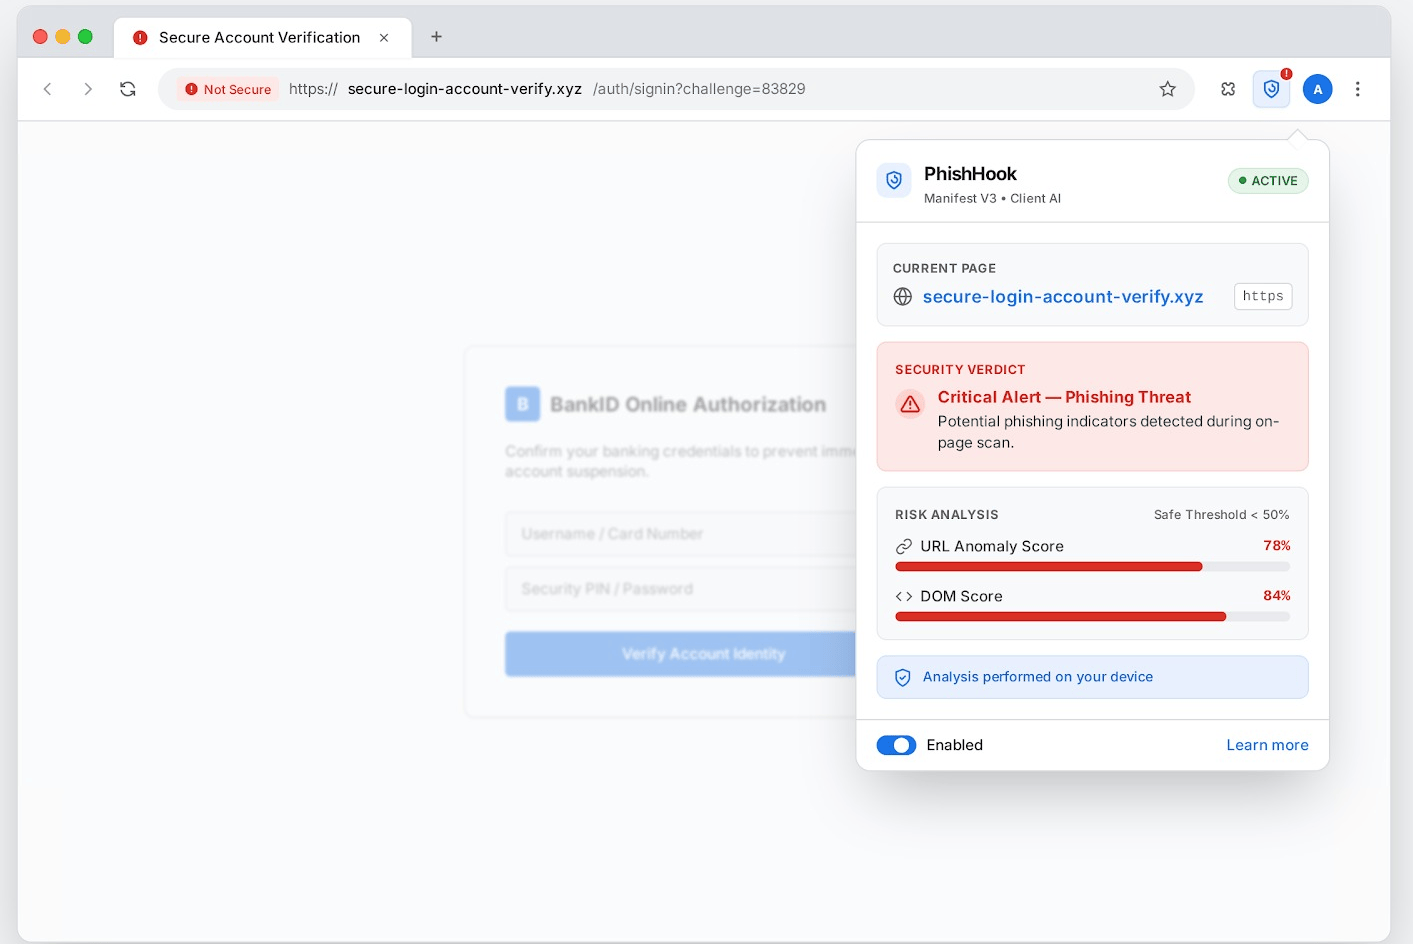
\includegraphics[width=0.90\linewidth,height=0.32\textheight,keepaspectratio]{Figures/gui_popup.png}
    \caption{Extension popup showing status and current verdict.}
    \label{fig:gui-popup}
\end{figure}

\subsection{Web Phishing Warning Banner}

The warning banner appears at the top of a web page when the fused risk score exceeds the deployed threshold. It informs the user that the page may be a phishing attempt and can be dismissed.

\begin{figure}[H]
    \centering
    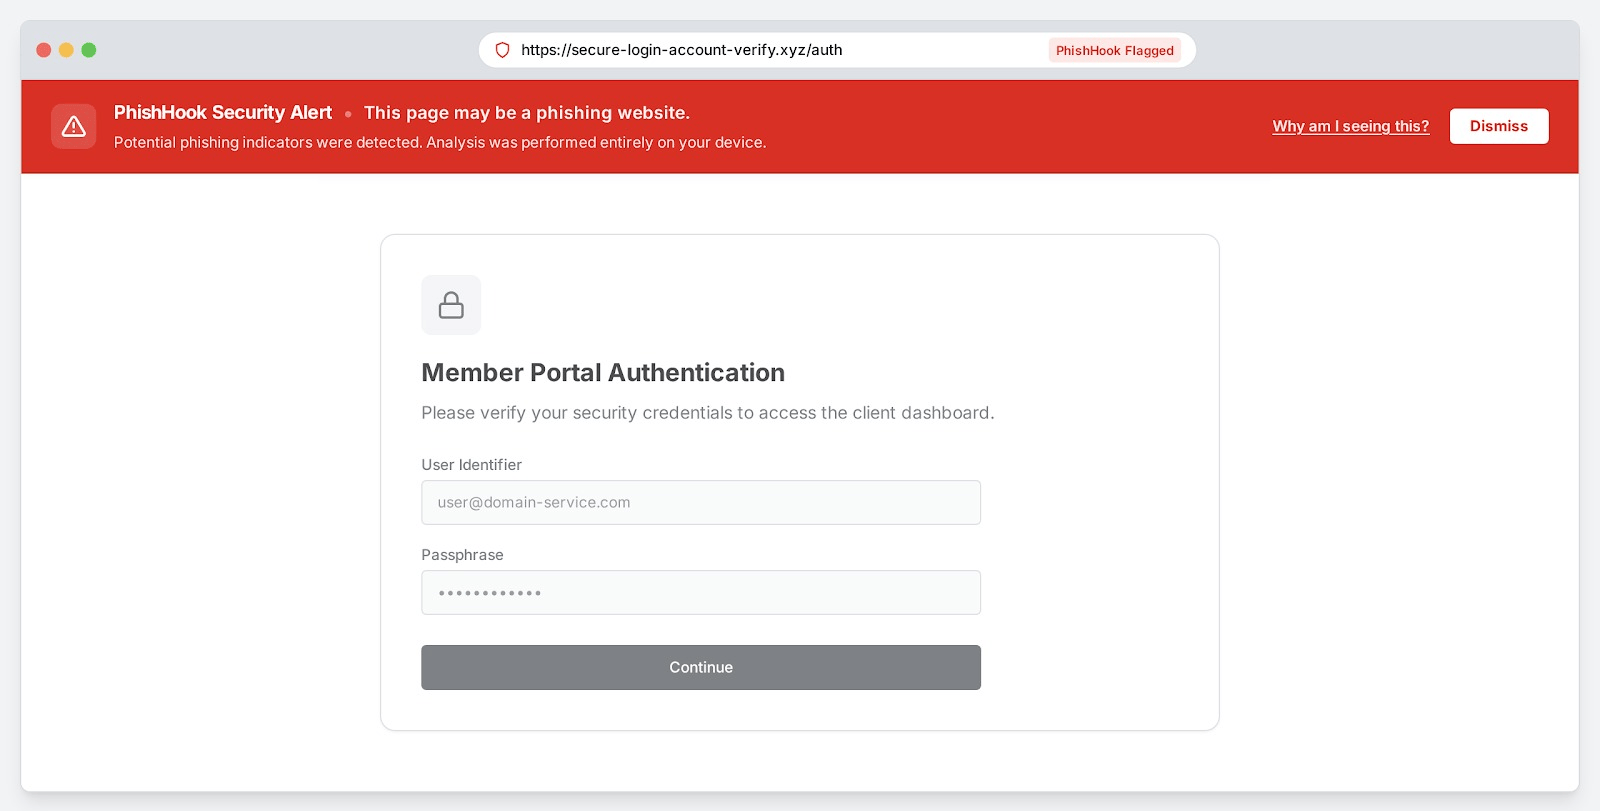
\includegraphics[width=0.95\linewidth,height=0.28\textheight,keepaspectratio]{Figures/gui_banner_web.png}
    \caption{Phishing warning banner displayed on a web page.}
    \label{fig:gui-banner-web}
\end{figure}

\subsection{Form Submission Warning}

When a user tries to submit a form on a page flagged as suspicious, the extension displays a stronger warning to highlight the potential risk. This gives users a final chance to review their decision and avoid sharing sensitive information with potentially unsafe websites. The warning also allows users to cancel the submission or proceed if they choose to accept the risk, keeping the final decision in their hands.

\begin{figure}[H]
    \centering
    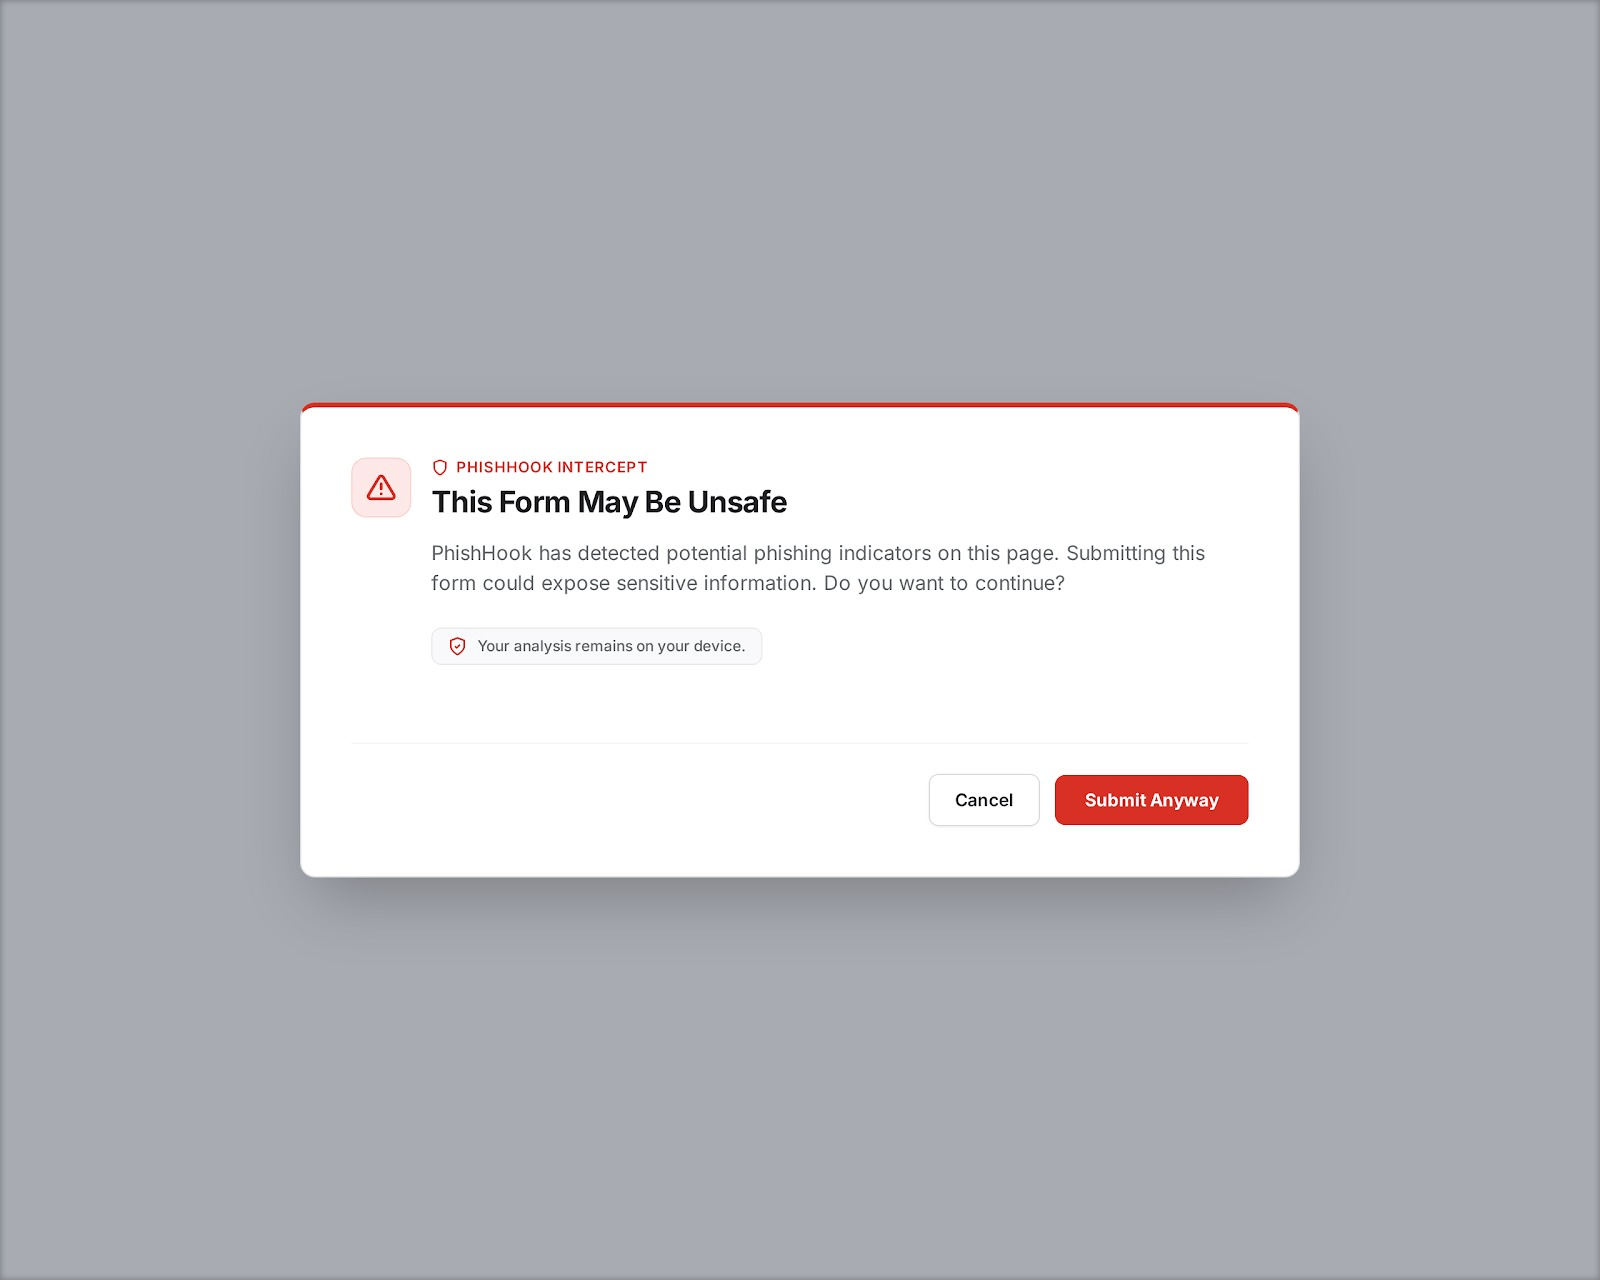
\includegraphics[width=0.85\linewidth,height=0.30\textheight,keepaspectratio,trim=230bp 295bp 230bp 295bp,clip]{Figures/gui_banner_form.png}
    \caption{Warning displayed when submitting a form on a suspicious page.}
    \label{fig:gui-banner-form}
\end{figure}

\subsection{Email Phishing Warning Banner}

The email warning is displayed within Gmail or Outlook web when the distilled BiLSTM student model detects a potentially phishing message. It helps users recognise suspicious emails and stay cautious while reading them, providing an additional layer of protection against email-based threats.

\begin{figure}[H]
    \centering
    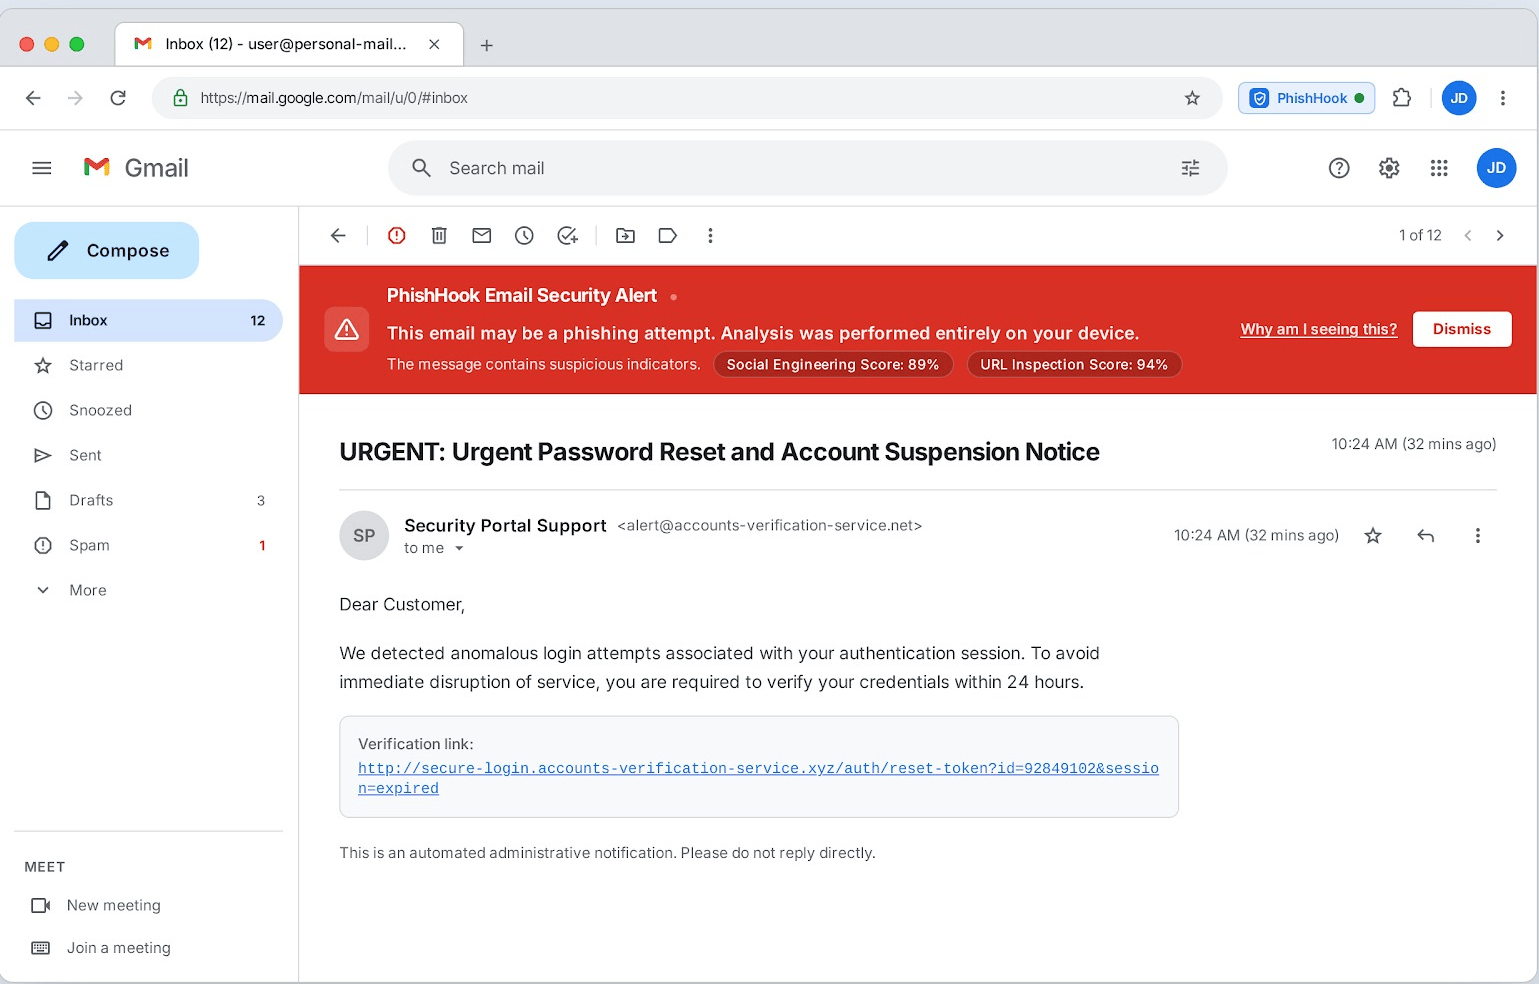
\includegraphics[width=0.95\linewidth,height=0.30\textheight,keepaspectratio]{Figures/gui_banner_email.png}
    \caption{Email phishing warning banner displayed in webmail.}
    \label{fig:gui-banner-email}
\end{figure}

\section{Risk Analysis}

The extension makes detection decisions using data available at the time of browsing. Its risk analysis therefore considers both model errors and problems in the surrounding browser workflow. A model may misclassify unfamiliar attacks, while changes to browser or webmail interfaces may interrupt input collection even when the model itself works correctly.

The analysis also considers the risks of excessive permissions, unsafe handling of sensitive inputs, and resource consumption during local inference. These risks are directly related to the requirements for limited permissions, provisional verdicts when inputs are incomplete, and resource measurement on the target hardware.

The following subsections distinguish risks arising from development data, browser operation, and changes over time. Each risk is linked to an appropriate check, such as testing on held-out data, evaluating fallback behaviour, or measuring the effect of repeated scans.


\subsection{Technical Risks}
The effectiveness of PhishHook depends on the quality and diversity of the datasets used to train and evaluate its phishing detection models. Biased, outdated, or insufficient datasets may cause poor generalisation and increase false-positive or false-negative rates. The datasets come from public sources including PhishPedia, PhishTank, Tranco, and the merged MeAJOR email corpus, and email datasets in particular may contain personal information even after cleaning, which raises data-leakage concerns during training. 

\subsection{Model Performance Risks}
PhishHook analyses URLs, webpage content, and email. Errors in a model or in score fusion can lead to incorrect verdicts. Good performance on a test dataset may not carry over to previously unseen phishing attacks.

\subsection{Browser Compatibility and Resource Risks}
Running models inside a Chrome extension comes with certain limitations, particularly in terms of model size, memory usage, inference time, and browser compatibility. Larger models can slow down page analysis and affect the overall browsing experience. Since the extension runs alongside other browser processes, it also needs to manage available system resources carefully. This makes model optimisation important to ensure that detection remains fast without putting too much load on the browser. Therefore, finding a balance between model accuracy, size, and execution speed is an important part of the deployment process.

\subsection{Security Risks}
PhishHook needs access to page data to detect phishing. Excessive permissions or poor handling of extracted data can expose users to security risks. Malicious or manipulated pages may disrupt extraction or trigger too many analyses.

\subsection{Adversarial Evasion Risks}
Anyone can inspect the models bundled with the extension. Attackers may use that access to craft phishing pages the detector classifies as benign. This risk is inherent in local detection and cannot be eliminated.

\subsection{Ethical and Privacy Risks}
PhishHook processes potentially sensitive webpage content, URLs, and emails. Storing those data unintentionally or handling them improperly could compromise user privacy.

\subsection{Operational and Maintenance Risks}
Chrome, Manifest V3 APIs, webmail interfaces, and inference dependencies can change and disrupt the extension. Detection may also become less effective as phishing techniques evolve. To manage this, the extension needs a plan for updating the model and fixing broken integrations whenever Chrome pushes a major update. We also have to keep watching for new obfuscation tricks that bypass the current DOM parser.

\section{Conclusion}
The requirements in this chapter describe how PhishHook analyses webpages and webmail, runs its models locally, and communicates verdicts during ordinary browsing. The feature and use-case descriptions connect user actions to the functional requirements, while the hardware, software, and interface sections record the conditions under which the extension is expected to operate. Privacy, security, reliability, efficiency, portability, and usability apply alongside detection accuracy. For example, the extension needs to handle missing content without giving a false impression of safety, and its warnings need to inform users while allowing ordinary browsing to continue. The assumptions identify what the extension expects from the browser and the supported webmail interfaces. The risk analysis describes where dataset quality, browser changes, limited resources, or model errors could affect the intended behaviour. These requirements set out what the methodology and design must account for, from the inputs available to the detector to the evidence needed to assess its performance in a browser.

\chapter{Proposed Approach and Methodology}
\label{ch:methodology}

This chapter describes the methodology used to build and evaluate PhishHook, a client-side phishing detector for Chromium browsers that extends PhishLang \cite{phishlang2026}. It first presents the overall framework and briefly states what PhishHook keeps from PhishLang and what it changes. It then presents the data sources and how the data is prepared. The central part of the chapter explains how the URL and the rendered page are acquired and parsed on the user's device, including how JavaScript-generated content and dynamic page changes are handled. The chapter then details the algorithms behind each module, an unsupervised URL anomaly detector, a supervised page-content classifier, a fusion model, and a distilled email classifier. It also defines the model comparisons, evaluation metrics, statistical tests, resource measurement protocol and adversarial tests used to judge the design. (Chapter~\ref{ch:design}).

\section{Overview of the Proposed Framework}
\label{sec:framework}

PhishHook is a framework made of an input acquisition stage followed by independent detection modules whose outputs are combined into one verdict. It runs entirely inside a Manifest V3 browser extension. It uses only two local sources: the URL string of the page the user has loaded and the already-rendered Document Object Model (DOM) of that page. It never fetches pages itself, performs no WHOIS, DNS, domain-age, search-index or reputation lookups, and transmits nothing off the device.

PhishHook extends PhishLang \cite{phishlang2026}, a fully client-side phishing detection framework that uses MobileBERT over a compact, structured representation of a page's actionable elements. PhishHook keeps that fully-local, transformer-based page-classification core and adds five things that PhishLang does not do. First, the URL is handled by a separate unsupervised module, and the URL itself is excluded from the DOM model's input so that the two modules stay complementary. Second, the two scores are combined by a small calibrated fusion model, trained on scores that are out of sample for the DOM model. Third, dynamic changes to the page after load are observed, and significant changes trigger re-analysis. Fourth, results are reported at low false-positive rates, at stated base rates, and on source-disjoint and temporal test sets. Fifth, an email surface is added using knowledge distillation from a MobileBERT teacher into a compact BiLSTM student. Resource cost is measured inside the extension on both high-end and low-end hardware.

The framework works through two user-facing surfaces.
\begin{itemize}
    \item On web pages, an unsupervised module checks the URL for anomalies while a supervised classifier examines the page's DOM. A small fusion model then merges the two scores into one risk score.
    \item On webmail, a compact BiLSTM student classifies the email being viewed. It was trained by distillation from a MobileBERT teacher.
\end{itemize}

\begin{figure}[!ht]
\centering
\resizebox{\textwidth}{!}{%
\begin{tikzpicture}[
    node distance=0.5cm and 0.6cm,
    box/.style={draw, rounded corners, align=center, minimum height=1.0cm, text width=2.3cm, font=\footnotesize, fill=blue!5},
    off/.style={draw, dashed, rounded corners, align=center, minimum height=1.0cm, text width=5.4cm, font=\footnotesize, fill=gray!10},
    arr/.style={-{Latex}}
]
% web row
\node[box] (page) {Loaded web page};
\node[box, right=of page] (extract) {URL parser and DOM parser};
\node[box, right=of extract, yshift=0.9cm] (url) {URL anomaly module};
\node[box, right=of extract, yshift=-0.9cm] (dom) {DOM classifier (MobileBERT, int8)};
\node[box, right=of url, yshift=-0.9cm] (fuse) {Fusion (logistic regression)};
\node[box, right=of fuse] (verdict) {Verdict and warning};
\draw[arr] (page) -- (extract);
\draw[arr] (extract) -- (url);
\draw[arr] (extract) -- (dom);
\draw[arr] (url) -- (fuse);
\draw[arr] (dom) -- (fuse);
\draw[arr] (fuse) -- (verdict);
\draw[arr, dashed] (extract.south) |- ++(0,-1.9cm) -| (verdict.south) node[pos=0.25, below, font=\scriptsize]{URL-only fallback if DOM unavailable};
% email row
\node[box, below=3.2cm of page] (mail) {Webmail page};
\node[box, right=of mail] (mparse) {Email parser};
\node[box, right=of mparse] (student) {BiLSTM student (distilled)};
\node[box, right=of student] (mverdict) {Email verdict};
\draw[arr] (mail) -- (mparse);
\draw[arr] (mparse) -- (student);
\draw[arr] (student) -- (mverdict);
% offline
\node[off, below=0.9cm of student] (offline) {Offline only (not deployed): MobileBERT teacher, reference baselines};
\draw[arr, dashed] (offline.north) -- (student.south) node[midway, right, font=\scriptsize]{distillation};
\end{tikzpicture}%
}
\caption{Overview of the PhishHook framework. Solid boxes run inside the browser extension; the dashed box is used only during training and comparison.}
\label{fig:framework}
\end{figure}

\begin{table}[!ht]
\centering
\caption{Deployed and offline-only components.}
\label{tab:components}
\begin{tabularx}{\textwidth}{|>{\raggedright\arraybackslash}X|>{\raggedright\arraybackslash}X|>{\raggedright\arraybackslash}X|}
\hline
\textbf{Component} & \textbf{Role} & \textbf{Deployed in extension?} \\
\hline
URL anomaly model (autoencoder or Isolation Forest) & Scores the URL string; trained on benign URLs only & Yes (the selected one) \\
\hline
DOM MobileBERT (int8) & Classifies parsed page text; the URL is excluded from its input & Yes \\
\hline
Fusion model & Combines the two web scores & Yes \\
\hline
BiLSTM student & Classifies emails visible in the webmail interface & Yes \\
\hline
MobileBERT teacher (email) & Produces soft labels for distillation & No (training only) \\
\hline
Reference baselines (K-Means/IF URL baseline, MobileBERT on URL strings, LightGBM on DOM features) & Measure what a simpler or supervised method achieves & No (comparison only) \\
\hline
\end{tabularx}
\end{table}

\section{Datasets and Data Preparation}
\label{sec:data}
This section describes the datasets used to develop and evaluate the PhishHook detection system. It covers the sources of the collected data, the steps taken to clean and prepare it, and how the data was organised for model training and testing. These steps help ensure that the models are trained on suitable data and can identify phishing attempts more reliably.
\subsection{Data Sources}
Five data sources support the experiments in this study, covering web pages, URLs, and emails. Each source has a specific role in training or testing, and these roles are listed below.
\begin{itemize}
    \item PhishPedia \cite{phishpedia2021} is a labelled web phishing dataset in which phishing and benign pages come with their URLs and HTML. It is used to train the supervised page-content model and to run the in-distribution tests.
    \item PhishTank is a community-driven phishing feed. The reported phishing URLs are crawled to collect each URL together with its rendered DOM, and the result serves as a source-disjoint and temporal test set.
    \item The benign URLs come from deeper-ranked domains on the Tranco list, combined with real URL paths taken from public crawl indexes or from links found on benign pages. They train the unsupervised URL module and are used to measure the FPR.
    \item PhiUSIIL is a phishing URL dataset with 134,850 legitimate and 100,945 phishing URLs, each described by 56 features drawn from the URL and the page source. It is the main dataset for training and evaluating the unsupervised URL anomaly module.
    \item MeAJOR \cite{meajor2025} is a merged, multi-source email phishing dataset that is used for the email study.
\end{itemize}

\subsection{Data Roles and Separation Principles}
\label{sec:roles}
The exact size of each split is fixed in the experimental plan. Whatever the final division turns out to be, the roles and rules below apply to every part of the data.
\begin{itemize}
    \item The training data is used to fit the model and learn its weights, and it supplies the examples from which the model picks up relevant patterns.
    \item The tuning data is used to adjust hyperparameters and to decide when training should stop. It lets performance be monitored during development and guides the choice of the final training setup.
    \item The calibration and fusion data is kept apart from DOM model training so that the scores are produced on unseen samples. It is used to calibrate the DOM model, train the fusion model, and select decision thresholds. This separation stops the calibration from benefiting unfairly from samples the model has already seen.
    \item The test data is reserved for the final evaluation. It contains an in-distribution test set, a source-disjoint and temporal test set, and a small collection of pages captured during real browsing sessions, which together show how the system behaves under familiar and less familiar conditions.
    \item The unsupervised URL model is trained on benign URLs only, and phishing URLs are left out of training. A separate benign validation set provides the reference scores for percentile ranking and threshold selection, so unusual URL patterns can be found without phishing labels.
    \item Samples and their near-duplicates, including those from the same domain or phishing campaign, are kept in the same split. Test data is never used for model selection, hyperparameter tuning, threshold selection, or calibration, so the final evaluation gives a fair view of how well the system generalises.
\end{itemize}

\subsection{PhishTank Collection Protocol}
Collecting live phishing pages carries security risks and can produce noisy data. A fixed procedure is therefore followed for every collection run, as described below.
\begin{itemize}
    \item All pages are opened in an isolated, disposable browser environment instead of a personal computer or account.
    \item No login credentials or personal information are entered on any phishing page.
    \item The submission timestamp given by the feed is recorded so that the time order of the pages can be preserved.
    \item Each page is opened in a real browser so that its JavaScript can run, and the resulting DOM and URL are then saved.
    \item Pages that are no longer active, parked, empty, showing errors, or clearly cloaked are excluded, and the number of excluded pages is recorded.
    \item Community feeds may contain wrong labels, so a random sample of the collected pages is checked manually to estimate the labelling error.
\end{itemize}

\subsection{Benign URL Set and Popularity Bias}
An anomaly detector trained only on benign URLs may wrongly flag less popular domains, or URLs that contain paths, as suspicious. Three measures are included to reduce this problem.
\begin{itemize}
    \item The benign training set contains domains beyond the most popular rankings, as well as URLs with real paths and query parameters.
    \item The evaluation is split into homepage-only URLs and URLs with paths or queries, which shows whether the model leans too heavily on URL structure.
    \item In an ablation study, paths and query parameters are removed from every URL before scoring, to see how much performance depends on them.
\end{itemize}
If no suitable source of less popular benign URLs can be found, this limitation will be stated clearly in the report.

\subsection{Cleaning and Deduplication}
Duplicates are removed at the URL, domain, and campaign level. The benign URL training data is also deduplicated against all other benign data used anywhere in the study. As a result, no URL that trains the unsupervised model is later used to measure its FPR, which keeps the false-positive estimates honest.

\subsection{Mapping Emails to the Webmail View}
\label{sec:email-mapping}
MeAJOR stores emails in their original form, but the extension can only see what a webmail page displays. To keep the training data consistent with what the extension can observe, every email is converted into a webmail-style representation before training. The conversion follows the rules below.
\begin{itemize}
    \item The subject line is kept as plain text.
    \item Only the sender's display name and the email address visible on screen are kept, without relying on hover information.
    \item The HTML body is converted into visible text, and scripts, styles, tracking pixels, and hidden elements are removed.
    \item Both the displayed link text and the destination host are retained for every link.
    \item Only the attachment file names shown in the webmail interface are included.
    \item Email headers are excluded completely, so training never uses information the extension cannot access.
\end{itemize}

\subsection{Required Benign Sample Size for False-Positive Estimates}
\label{sec:fpr-size}
The evaluation focuses on low FPR values, and these need many benign samples to be estimated reliably. The number of benign samples required is given by
\begin{equation}
n \;\ge\; \frac{1-p}{p\, r^{2}},
\label{eq:fpr-size}
\end{equation}
where $p$ is the target FPR, $r$ is the acceptable relative standard error, and $n$ is the number of benign samples. As Equation~\ref{eq:fpr-size} shows, a smaller target FPR requires many more samples. For $r = 0.2$, about 2{,}475 samples are needed for $p = 1\%$ and about 24{,}975 samples for $p = 0.1\%$.

\section{Input Acquisition and Parsing}
\label{sec:input-acquisition}
This section explains how the extension obtains the URL and the page content on the user's device and turns them into model inputs. The same procedures are applied when the training data is prepared, so that both stages see inputs in the same form.

\subsection{What Is Read and When}
The extension reads two inputs from every page, and each one is collected at a specific moment.
\begin{itemize}
    \item The URL of the main page is taken from the browser's navigation information once the navigation has finished.
    \item The content script collects the rendered DOM after the page has finished loading and its content has become stable.
\end{itemize}

\subsection{URL Acquisition and Parsing}
\label{sec:url-parsing}
The original URL is kept exactly as the browser reports it for the unsupervised character-level model. A separate parsed copy is prepared for the feature-based model through the steps below.
\begin{itemize}
    \item The URL is divided into its main parts: the scheme, host, port, path, query, and fragment.
    \item For the host, the number of subdomain levels, host labels, and hyphens is counted, and the parser checks whether the host is an IP address.
    \item Internationalised domain names are decoded from their punycode form, and the presence of punycode is stored as a separate feature.
    \item The path is split into segments and the query string into parameters, and the number of each is recorded.
    \item Percent-encoded characters are identified and their decoded forms are used for the statistics, while the original URL is kept for the character-level model.
    \item Length, digit ratio, and character entropy are calculated separately for the host, path, and query, and the longest run of consecutive digits is recorded.
    \item The frequency rank of the top-level domain is looked up in a reference table built from the benign training data.
    \item The scheme (\texttt{http} or \texttt{https}) is left out of the feature set, because it may reflect when a dataset was collected and not whether a URL is malicious.
\end{itemize}

\subsection{Rendered DOM Acquisition}
\label{sec:dom-acquisition}
The content script reads the live, rendered DOM and not the original HTML source that the browser downloaded. This lets the system work with the page as the user sees it, after scripts and other dynamic changes have run. The reading rules differ slightly depending on where the content sits.
\begin{itemize}
    \item The complete rendered DOM of the main page is read, including elements that scripts added, moved, or changed after the initial load.
    \item Frames that share the origin of the main page are read as well, and their content is treated as part of the main page.
    \item The browser blocks access to frames from a different origin, so only the source host of such a frame is recorded. This is a known limitation, because phishing forms placed inside these frames cannot be read by the parser.
    \item Open shadow roots are traversed and their content is added to the extracted text. Closed shadow roots cannot be reached by external scripts, so anything inside them stays unavailable to the parser.
\end{itemize}

\subsection{DOM Parsing and Serialisation Algorithm}
\label{sec:dom-parsing}
The parser does not give MobileBERT the raw DOM or raw HTML. Instead, it builds a small, organised model of the page elements that matter, following the approach of PhishLang \cite{phishlang2026}. The process works as follows.
\begin{itemize}
    \item The parser walks through the rendered DOM depth-first and stops after a fixed number of nodes, so very large pages cannot slow down or freeze the browser.
    \item Scripts, styles, comments, and template elements are skipped, since they hold nothing that the user can see directly.
    \item Elements that are hidden, not displayed, of zero size, or positioned far outside the visible area are also skipped. Attackers may place hidden text or form fields on a page to mislead a model with content that users never see, so focusing on visible elements reduces this risk.
    \item The feature groups listed in Table~\ref{tab:dom-groups} are collected from the remaining visible elements. Each group covers a type of page element that can help detect phishing, in line with the feature extraction used by PhishLang.
    \item The extracted text is normalised by reducing repeated spaces, removing control characters, and dropping exact duplicate entries.
    \item Each feature group is turned into a short labelled text segment, such as \texttt{TITLE: ...}, \texttt{FORMS: ...}, or \texttt{ANCHORS: ...}, and the segments are joined in a fixed priority order.
\end{itemize}
The parser works with extracted features instead of the entire raw DOM for several reasons. A complete DOM can easily exceed the 512-token limit of MobileBERT, and simply cutting off the extra content could remove details that help to recognise a phishing page. Choosing specific feature groups also guarantees that the most important elements, especially the page title and the login form, reach the model even when a page contains a large amount of content. Finally, this approach drops styling, layout information, and repeated page content that add nothing to phishing detection. The model therefore receives a smaller and more focused view of the page.

\begin{table}[!ht]
\centering
\caption{Element groups extracted from the rendered DOM, in priority order.}
\label{tab:dom-groups}
\begin{tabularx}{\textwidth}{|c|>{\raggedright\arraybackslash}X|>{\raggedright\arraybackslash}X|}
\hline
\textbf{Priority} & \textbf{Group} & \textbf{What is extracted} \\
\hline
1 & Title and headings & The page title and the main visible headings \\
\hline
2 & Brand cues & Alternative text and labels of logos and images \\
\hline
3 & Forms and inputs & Field labels, placeholders, field names and types, button text \\
\hline
4 & Anchors (HREFs) & Visible link text and the destination host only; repeated hosts counted once \\
\hline
5 & Scripts and iFrames & The presence of these elements and the source hosts of frames \\
\hline
6 & Footer and helper links & Policy, help and account links \\
\hline
7 & Visible body text & Remaining visible text, deduplicated, in reading order \\
\hline
\end{tabularx}
\end{table}

The URL of the page is deliberately left out of this representation. The URL module sees only the URL, and the DOM module sees only the page content, so the two modules stay complementary and the fusion stage has two independent signals to combine. If the URL were added to the DOM model's input, the two modules would overlap and the fusion would add no value.

\subsection{Token Budget and Truncation}
\label{sec:token-budget}
MobileBERT accepts at most 512 tokens. To stay inside this limit while keeping the most useful page information, the serialised representation is reduced with the rules below.
\begin{itemize}
    \item Each of the seven groups in Table~\ref{tab:dom-groups} has a maximum number of items, so a single group with many elements cannot use up most of the token space.
    \item The groups are joined in the priority order of Table~\ref{tab:dom-groups}, with the title, brand cues, forms, and inputs first and the visible body text towards the end.
    \item If the combined text still exceeds 512 tokens, content is cut from the end. The less informative groups sit last, so the information most relevant to phishing detection is kept.
    \item Page-size information is not given to the model. Together with the per-group item limits, this prevents the model from using page size as a shortcut.
\end{itemize}
Because the title, brand cues, forms, and inputs come first, they survive even when truncation is needed. How often truncation happens, and which groups it affects most, is measured and reported.

\subsection{Handling JavaScript-Rendered and Dynamic Content}
\label{sec:js-dynamic}
Phishing pages often use JavaScript to show content or to change the page after it has first loaded. The extension handles such dynamic content in the following ways.
\begin{itemize}
    \item The content is read from the live DOM after the page's load event, and not from the initial HTML.
    \item After the load event, the extension waits for a short period in which no relevant changes occur, and a maximum waiting time prevents unnecessary delays.
    \item A mutation observer watches the page for newly added or removed elements and for changed attributes after the first analysis.
    \item In single-page applications, an address change without a full reload is treated as a new page, and the analysis starts again from the beginning.
    \item DOM traversal is split into smaller tasks that run during the page's idle time, which limits interference with normal browsing.
\end{itemize}

\subsection{Dynamic Monitoring and Re-Trigger Policy}
\label{sec:dynamic-trigger}
Analysing every change made to a page would cost a lot of unnecessary processing, so the extension starts a new analysis only when a change is significant. Six types of change are monitored. First, a password field or a new form that appears or becomes visible counts as significant, since collecting login credentials is a common goal of phishing pages. Second, a noticeable change in the number of visible input fields may show that a login form was added after loading. Third, changes to the page title or to the brand-cue elements are watched because they can signal a change in the identity of the page. Fourth, a frame added with a new source matters because it may bring in content from another origin. Fifth, replacing a large part of the visible content may mean that the page has been rebuilt. Finally, a client-side route change is treated as a new event, since it may show a different page without a full reload.

Once one of these changes is detected, the re-analysis proceeds as follows. This ensures that the system uses the latest available page information before updating its detection result and displaying the corresponding warning to the user.
\begin{itemize}
    \item The mutation observer reports a change on the page.
    \item The extension checks whether the change matches one of the six significant types, and all other changes are ignored.
    \item Several events are grouped together by debouncing, and the analysis starts only after the page has stayed unchanged for a short interval.
    \item A cool-down period and a maximum number of analyses per page keep the processing cost under control.
    \item If an analysis is already running, the newest request replaces any older request that is still waiting.
    \item When the new analysis finishes, the earlier verdict is updated, and if a page changes from benign to suspicious, a warning is shown at that point.
\end{itemize}

\subsection{Parsing Webmail Content}
\label{sec:email-parsing}
Email content is read directly from the DOM of the webmail page, using a separate adapter for each supported client, namely Gmail and Outlook web. Each adapter finds the email that is currently open and collects the same fields that are used in the training data mapping. For every link, the extension also checks whether the host shown in the link text matches the real destination host. It never opens a link or follows its destination, so every link is judged from its address and the text around it.

\subsection{Training--Deployment Parity}
\label{sec:parity}
The parser used inside the extension is also applied to the training pages, so that both stages process data in the same way. When a dataset contains only downloaded HTML, the page is first opened in a real browser so that its scripts can run and produce the rendered DOM, which is then passed to the parser. A small collection of pages captured during real browsing sessions is additionally kept as a separate test set, to check how the system performs on pages from everyday use.

\section{Module A: Unsupervised URL Anomaly Detection}
\label{sec:url-module}
This module looks for unusual URLs by learning the patterns found in benign web addresses. Unlike supervised approaches, it does not use phishing URLs during training. It learns what normal URLs look like and gives higher anomaly scores to URLs that differ from those patterns. Two candidate models and one baseline are compared to find out how well this idea works. The comparison also helps determine which approach can identify unusual URL patterns more effectively while keeping false alarms to a reasonable level. This helps assess whether the models can recognise suspicious URLs even when they contain patterns not seen during training.

\subsection{Problem Formulation}
Let $u$ be a URL. The module assigns it an anomaly score $s(u)$, where a higher value means that the URL differs more from the benign URLs seen in training. A URL is marked as anomalous when its score is above a threshold $\tau$. This threshold is selected on benign validation data so that it reaches the target FPR values of 1\% and 0.1\%.

\subsection{Candidate 1: Character-Level Autoencoder}
The first candidate maps each character of a URL to an index from a fixed vocabulary. Every URL is then brought to a fixed length $L$ by cutting longer URLs or padding shorter ones, and a mask marks the padded positions so that they are left out of the calculations. A convolutional encoder compresses the character sequence into a compact latent representation, and a decoder rebuilds the sequence by predicting a probability distribution over the vocabulary at each position.

Let $c_i$ be the actual character at position $i$, $p_i(c_i)$ its predicted probability, and $M$ the set of positions that do not contain padding. The reconstruction loss, which is also used as the anomaly score, is
\begin{equation}
s(u) \;=\; -\frac{1}{|M|}\sum_{i\in M} \log p_i(c_i).
\end{equation}
The model is trained to minimise this loss on the benign training URLs, so URLs that look unfamiliar to it should produce higher reconstruction errors. Because the error can change with URL length and character variety, performance is also evaluated separately for different length groups.

\subsection{Candidate 2: Isolation Forest on Lexical Features}
The second candidate uses the lexical features described in Section~\ref{sec:url-parsing}. These include separate statistics for the host, path, and query, together with the subdomain depth, path depth, query parameter count, hyphen and dot counts in the host, the longest run of digits, the punycode and percent-encoding flags, and the top-level domain rank.

Isolation Forest finds unusual samples by measuring how easily they can be separated from the rest of the data. For a sample $x$ and a training sample size $n$, the anomaly score is
\begin{equation}
s(x,n) \;=\; 2^{-\,E[h(x)]/c(n)},
\end{equation}
where $h(x)$ is the number of splits needed to isolate $x$ and $E[h(x)]$ is the average path length over all trees. The term $c(n)$ is the expected path length of an unsuccessful search in a binary search tree with $n$ points, and scores close to 1 point towards an anomaly. To see how much each feature group contributes, the model is also evaluated with one group removed at a time, covering the host, path, query, top-level domain, and encoding features. The resulting changes in performance show which groups matter most for anomaly detection.

\subsection{Candidate 3: K-Means Distance Baseline}
As an extra baseline, a K-Means model is trained on the same benign lexical features, and each URL is scored by its distance to the nearest cluster centroid. This gives a simple point of reference for judging the two main candidates against a basic clustering method. The K-Means model is used only for comparison and is not part of the deployed system.

\subsection{Testing the Unsupervised Approach}
Six tests are used to examine how well the unsupervised approach works.
\begin{itemize}
    \item A separation test checks whether benign and phishing URLs have clearly different score distributions in the validation data.
    \item A training-set composition test compares models trained on top-ranked benign domains only with models trained on deeper-ranked benign URLs.
    \item A training-set size test measures how performance changes as more benign training data is added.
    \item A path and query ablation removes both parts from every URL and compares the results.
    \item A length analysis reports scores and detection rates by URL length band.
    \item A shift robustness test evaluates the models on the source-disjoint and temporal test sets.
\end{itemize}

\subsection{Supervised Reference Model and URL Comparison}
\label{sec:url-comparison}
To see what the unsupervised module does well and where it falls short, it is compared with a supervised model on the same task and the same test data. MobileBERT is fine-tuned on the raw URL text to separate phishing from benign URLs. This supervised model is used only for comparison and is never deployed in the extension. The deployed DOM classifier is a different model that looks at page content and never sees the URL.

Four URL models are compared in total. The Isolation Forest and the character-level autoencoder are both trained on benign URLs only, and they are the unsupervised candidates for deployment. The K-Means distance baseline is also trained on benign URLs only, and it shows whether the Isolation Forest is actually better than a simpler method. The MobileBERT model on URL strings is trained on labelled URLs and acts as the supervised reference.

The comparison has to be read fairly. The supervised model sees phishing labels during training, so it is expected to do well on data similar to its training set. The more useful questions are how large the gap to the unsupervised models is at a low FPR, whether that gap grows when the data comes from a different source or a later time, and how the models differ in size and speed.

\subsection{Percentile-Rank Transformation}
Raw anomaly scores from different models cannot be compared directly. For fusion, the score of the selected model is therefore converted into a percentile rank among the benign validation scores $s_1,\dots,s_m$:
\begin{equation}
r(s) \;=\; \frac{1}{m}\,\bigl|\{\,j : s_j \le s\,\}\bigr| .
\end{equation}
About one thousand reference quantiles are stored in the extension, which is enough to compute the rank on the user's device without keeping the full validation set.

\section{Module B: Supervised DOM Classification}
\label{sec:dom-module}
This module classifies a page as phishing or benign from its content alone. It uses the serialised DOM representation described earlier and compares a fine-tuned MobileBERT model with a tree-based baseline. The subsections below describe the input, the baseline, the training procedure, the deployment format, and the comparisons that are carried out.

\subsection{Input and Model}
The model receives the serialised representation from Section~\ref{sec:dom-parsing}, which is built from the seven feature groups of Table~\ref{tab:dom-groups} and trimmed to the token budget of Section~\ref{sec:token-budget}. It returns a phishing score for the page. MobileBERT is fine-tuned for this binary classification task.

\subsection{Baseline Model: LightGBM}
A gradient-boosted tree model is trained on engineered features taken from the same seven DOM groups. The features include the number and types of form fields, the presence of a password field, the number of external link hosts, the number of iframes, the ratio of script nodes to all nodes, the number of brand-cue elements, specific keywords in the title, and page-length statistics. LightGBM is used for comparison only. It is not deployed and is not part of the fusion pipeline. Its results help show how well traditional feature-based methods perform compared to the other models. This comparison also provides a better understanding of which DOM features contribute most to distinguishing legitimate pages from phishing attempts.

\subsection{Fine-Tuning Procedure}
The model is fine-tuned on the training data, and its hyperparameters and early stopping point are chosen on the tuning data. The search budget and the random seeds are fixed in advance and reported, so that the results can be repeated and no model gains an advantage from extra tuning effort.

\subsection{Quantisation, Export and Parity}
The trained model is exported to a portable format for deployment and converted to 8-bit integers through quantisation. A 16-bit version is also evaluated to show the effect of an intermediate precision level. Accuracy, calibration, and model size are compared across the 32-bit, 16-bit, and 8-bit versions. A parity check then verifies that the exported model gives results consistent with the original model within a set tolerance.

\subsection{Model Comparison}
MobileBERT and LightGBM are evaluated on the same test sets with the same metrics, which keeps the comparison fair. Bootstrap confidence intervals are calculated for each comparison to account for variation in the results. The evaluation asks whether a lightweight transformer performs better than a traditional tree-based model when both use the same DOM-derived features. Model size and inference latency are also considered, to understand what any performance gain costs.

\subsection{Input Ablation}
To see how different input components affect the model's performance, it is trained and tested using several combinations of the available inputs. These include the full representation, title and brand cues only, title and brand cues with forms and inputs, and the same combination with anchors and scripts added. The model is also evaluated using only the visible body text and, as a control, the full representation with the URL included. Comparing these results helps identify which parts of the DOM provide the most useful information for phishing detection. It also shows whether adding more page elements improves performance or introduces unnecessary information. This comparison helps determine which input combination offers a good balance between detection accuracy and the amount of information processed.

\section{Module C: Fusion}
\label{sec:fusion}
The fusion module brings together the outputs of the URL and DOM modules to produce a single detection decision. It uses a lightweight model with very few parameters, keeping the additional processing cost low and allowing it to run efficiently within the browser extension. By combining information from both modules, it can make decisions based on different aspects of a web page rather than relying on a single source. This section explains the fusion model, the steps taken to prevent data leakage, the method used to select the decision threshold, and the comparisons carried out to evaluate its performance.

\subsection{Fusion Model}
Fusion takes two inputs: the percentile rank $r$ of the URL anomaly score and the calibrated DOM score $z_{\mathrm{cal}}$. A logistic regression turns them into a combined probability:
\begin{equation}
P(\text{phishing}) \;=\; \sigma\!\left(w_1\, r + w_2\, z_{\mathrm{cal}} + b\right),
\end{equation}
where $w_1$, $w_2$, and $b$ are three numbers fitted on held-out data, and $\sigma$ is the logistic function that maps any value to a probability between 0 and 1. Training minimises the negative log-likelihood plus a small penalty $\lambda\,(w_1^2 + w_2^2)$, which keeps the weights from overfitting the small fitting set. Only these three numbers and one threshold have to be stored in the extension.

\subsection{Leakage Control}
The fusion model is fitted only on data that was held out from the training of the DOM model. The DOM scores it sees are therefore genuinely unseen, and the fusion weights are not inflated by samples the DOM model has already learned.

\subsection{Decision Threshold and Fallback}
The decision threshold is chosen on the same held-out data so that it reaches the target FPR values, and it is not simply fixed at 0.5. If the page content is not available, the extension falls back to the URL score alone and applies a separate threshold for it.

\subsection{Ablations and Complementarity}
Four configurations are compared at the stated base rates: URL only, DOM only, an OR rule, and the fused model. Complementarity is measured through the correlation between the URL score and the DOM score, and through the gain in detection that fusion provides.

\section{Email Phishing Detection and Knowledge Distillation}
\label{sec:email}
Email detection operates within the webmail interface described earlier and uses a compact model designed to run directly in the browser. The process begins by training a larger teacher model, which is then used to guide a smaller student model through knowledge distillation. This allows the student model to retain useful detection capabilities while keeping its size and computational requirements low. The following subsections explain the models, their training process, and the checks performed to ensure that the final deployed model works as expected.

\subsection{Models in the Study}
Two models are used for the email task.
\begin{itemize}
    \item A MobileBERT teacher is fine-tuned on the email training data.
    \item A distilled BiLSTM student is trained from the soft labels of the teacher, and it is the email model that is deployed.
\end{itemize}

\subsection{Teacher and Student}
The teacher is fine-tuned on the training emails in their webmail view, and its calibration is checked, because the soft labels carry the teacher's confidence. The student is a bidirectional recurrent model with its own vocabulary and embeddings, made up of an embedding layer, a bidirectional LSTM layer, a pooling step, and an output layer. The teacher and the student use different tokenisations, so distillation is done at the output level only.

\subsection{Quantisation, Export and Parity}
The student model is exported in a portable format and quantised to 8-bit integers for deployment. A 16-bit version is also tested, and the three versions are compared in terms of accuracy, calibration, and model size. A parity check makes sure that the exported model produces results close to those of the original.

\subsection{Model Comparison}
The MobileBERT teacher and the distilled BiLSTM student are tested on the same email test data with the same evaluation metrics. Bootstrap confidence intervals are calculated for the comparison, and model size and inference latency are reported next to accuracy. This shows how much performance is given up in exchange for a student that is small and fast enough to run in the browser.

\subsection{Input Ablation}
To identify which parts of a webmail view are most useful for phishing detection, the models are tested using different combinations of the fields described in Section~\ref{sec:email-mapping}. These include the email subject, sender, body, links, and attachment names. Comparing the results helps determine which fields provide the most useful information for detecting phishing emails and how combining them affects overall detection performance.

\section{Consolidated Model Comparison Framework}
\label{sec:comparison}
The study answers its research questions through four comparisons, which are summarised in Table~\ref{tab:comparisons}. Each row names the models involved and the question that the comparison is meant to answer.

\begin{table}[!ht]
\centering
\caption{Comparisons carried out in the study.}
\label{tab:comparisons}
\begin{tabularx}{\textwidth}{|c|>{\raggedright\arraybackslash}X|>{\raggedright\arraybackslash}X|}
\hline
\textbf{ID} & \textbf{Models compared} & \textbf{Question answered} \\
\hline
C1 & Isolation Forest, character-level autoencoder, K-Means baseline, MobileBERT on URL strings (supervised reference) & How much does unsupervised URL detection lose against supervision, and which unsupervised model is better? \\
\hline
C2 & DOM MobileBERT at 32-bit, 16-bit and 8-bit, and its input ablations & How do numeric precision and input components affect accuracy, calibration and cost? \\
\hline
C3 & DOM MobileBERT, LightGBM on the same DOM features & Does a lightweight transformer outperform classical tree-based models on DOM-derived text, and at what cost? \\
\hline
C4 & URL only, DOM only, OR rule, fusion & Does fusion reduce false alarms compared with either module alone or a simple rule? \\
\hline
\end{tabularx}
\end{table}

All models within a comparison use the same data, the same metrics, an equal tuning budget, and several random seeds. Size and latency are reported next to accuracy, and the selection rules are fixed before the test sets are used.

\section{Conclusion}
\label{sec:method-conclusion}
This chapter set out the methodology for PhishHook. It described the data sources and the rules that keep training, calibration, and test data separate, and the procedures that extract and parse the URL and the rendered page on the user's device, including how hidden content is skipped and how dynamic page changes trigger re-analysis. It then defined the algorithms behind each module: an unsupervised URL anomaly detector with two candidate models, a supervised DOM classifier based on a quantised MobileBERT, a logistic-regression fusion model that combines the two scores, and a compact BiLSTM student trained by knowledge distillation from a MobileBERT teacher for email detection.


\chapter{High-Level and Low-Level Design}
\label{ch:design}
This chapter presents the high-level and low-level design of PhishHook. 

\section{System Overview}

PhishHook is a client-side phishing detection extension for Google Chrome (Manifest V3). It combines an unsupervised URL anomaly model with a supervised MobileBERT DOM classifier, fused by logistic regression, to produce a webpage verdict. For Gmail and Outlook web, a MobileBERT-distilled BiLSTM classifies emails. All models run locally through a WebAssembly runtime in an offscreen document and no user data leaves the device.

\subsection{System Design}

PhishHook consists of interconnected modules for URL processing, webpage analysis, classification, email inspection, and warning generation.

\subsubsection{URL and DOM Extraction}

The active page's URL is normalised using the training-time procedure. A text representation of the rendered DOM is built from the title, form field types and labels, link domains, iframes, script indicators, and visible text. Input values are never collected. Non-visible or hidden components are not considered in the extraction process because the model only accesses components that are visible to the user.

\subsubsection{Webpage Detection and Score Fusion}

An unsupervised model scores how unusual the URL is relative to benign URLs, and a MobileBERT classifier estimates phishing likelihood from the DOM. The URL anomaly percentile and DOM score are combined by a logistic regression meta-classifier trained on held-out scores. Configured thresholds map the fused score to benign, suspicious, or phishing.

\subsubsection{Email Phishing Detection}

When an email is opened on Gmail, the subject, sender details, body text, links, and attachment names are extracted. A small model name BiLSTM act as student distilled from main model called MobileBERT outputs a phishing probability on that basis it is decided that email is legitimate or phished. In case that probability passes the threshold set up then a dismissible warning pops up within the webmail page itself, and the content of the mail gets cleared out of memory.
\subsubsection{Dynamic Monitoring and Warning Generation}

The system will then rethrottle and re-inferve password fields, forms or iframes for a limited amount of time after loading a page to limit the overhead. The result will trigger a pop up in an isolated window, controlled by the extension.

\subsubsection{Email-to-Web Correlation}

The email verdict is associated with the page loaded via that email through a chrome tab opener relationship, but not through a URL match. A decision logic is a combination of these two verdicts to create an event ruling in a time period. Otherwise, the verdicts are kept independent.

\subsubsection{Local Inference and Privacy Management}

The models will be packaged along with the Extension and are local which mean that no URLs, Web page contents, or email contents will be sent to any external services. The data processing takes place only in memory and is erased once the inference is completed. In case of loading or timeout failure, the extension will not consider the page as safe.

\subsection{Data Collection}

Phishing web pages are collected from PhishPedia and PhishTank. For PhishTank, URLs are opened in a sandboxed environment in a browser and the resulting DOM is stored along with the URL and when it was submitted. The number of pages removed is reported including dead, parked, empty and error pages. The community provided labels can be noisy so a random sample is hand checked to estimate the label error rate. The benign URLs are from deeper ranked tranco domains, the URL module is based on the PhiUSIIL dataset, and emails are taken from the MeAJOR corpus. The URL model is only trained with benign URLs, the DOM classifier with labelled phishing and legitimate page representations, and the email model with labelled phishing and legitimate emails. In both training, deployment and preprocess is the same.

\subsection{Model Training}

The URL model learns from benign URLs, and frozen benign quantiles convert its scores to percentiles. The MobileBERT DOM classifier is compared offline against baselines such as XGBoost which are not deployed. The fusion meta-classifier is trained on held-out URL and DOM scores. For email, MobileBERT serves as teacher and distils into the BiLSTM student, which is the only email model deployed, email phshing detection model is also compared with other model to check the accuracy versus resource consumption trade off.
\section{Design Considerations}
\label{sec:design-considerations}

This section describes the assumptions, dependencies , constraints, and guidelines that shape the design of PhishHook.


\subsection{Assumptions}
\begin{itemize}
    \item The browser exposes the current URL and rendered DOM to the extension through standard MV3 APIs.
    \item The user has granted the host permissions required for the STRETCH email feature without them, email detection is disabled.
    \item Gmail and Outlook web DOM structures remain stable enough for the extraction selectors to work.
\end{itemize}

\subsection{Dependencies}
\begin{itemize}
    \item The system needs MV3 components and WebAssembly for local inference.
    \item The extension contains all the selected models and fusion rules so no remote code is loaded.
    \item Model quality depends on the labelled and benign datasets used for training and evaluation, and on consistent preprocessing between training and deployment.
    \item chrome.offscreen.createDocument requires a declared reason from Chrome's fixed list.
\end{itemize}

\subsection{General Constraints}
The following constraints come from the Manifest V3 platform, the model limits, and the privacy requirements of the system.

\subsubsection{Local-Only Operation}
PhishHook doesn't connect to the network. Doesn't transmit any telemetry, does no reputation lookups, and doesn't download models or code at runtime. New versions of a model are shipped via normal browser extension updates when it requires them.

\subsubsection{Privacy of Inputs}
The extension is not able to read typed data into text boxes or in other input field show in the web page. All content is in chrome memory only and the page's own URL is not part of the DOM input both the DOM and the URL are treated separately.

\subsubsection{Model Input Limit}
The DOM text is reduced to a maximum of 512 tokens, dropping the less relevant contents first, for MobileBERT.

\subsubsection{MV3 Service-Worker Lifetime}
A service work is closed if it is idle for more than approximately 30 seconds. Therefore, inference is performed in an offscreen document and the cost of reloading the model is measured.

\subsubsection{No Pre-Navigation Blocking}
Manifest V3 does not allow an ML decision to inhibit a navigation, so PhishHook can't block a page before it appears. It checks after page load, after DOM change and on form submission. A page that has not been analysed remains pending and is never marked safe.

\subsubsection{Memory and CPU}
Extension must be performed in a realistic budget in a low end laptop. MobileBERT is the largest model in the system, so its size and load time will be calculated after completing the WebAssembly experiments. Throttling, limiting the number of inferences, and a fixed monitoring window are all aspects of continuous DOM monitoring.


\subsection{Goals and Guidelines}
These are the goals PhishHook aims to achieve while staying within the constraints described above.

\begin{itemize}
    \item The extension must be auditable and it should ensure that no data is transferred out of the device.
    \item The URL module has only access to the URL, the DOM module has only access to the DOM.
    \item A page that is not analyzed is not reported as safe and when new evidence emerges, the verdict is raised later.
\end{itemize}

\subsection{Development Methods}
The design and development of PhishHook is iterative each major design decision is made through experimentation, not assumption. The decisions taken include the selection of the URL model, the representation of the DOM input, the supervised DOM model, the monitoring strategy and the representation of the fusion model. In most of them, two candidates are compared on the validation partition, the outcome is noted and only then does the next decision make. Candidates are measured against the same set of data, metrics, an equal tuning budget and a few random seeds. The test sets are used for the final reported numbers and to select a model, hyperparameter or threshold.

\section{System Architecture}
\label{sec:design-architecture}
The figure shown below is the architecture of PhishHook. It is a Chromium Manifest V3 extension running four models on the device a unsupervised URL anomaly model, a supervised MobileBERT classifier for the DOM, a small fusion meta-classifier and a distilled BiLSTM student for email.


\begin{figure}[H]
    \centering
    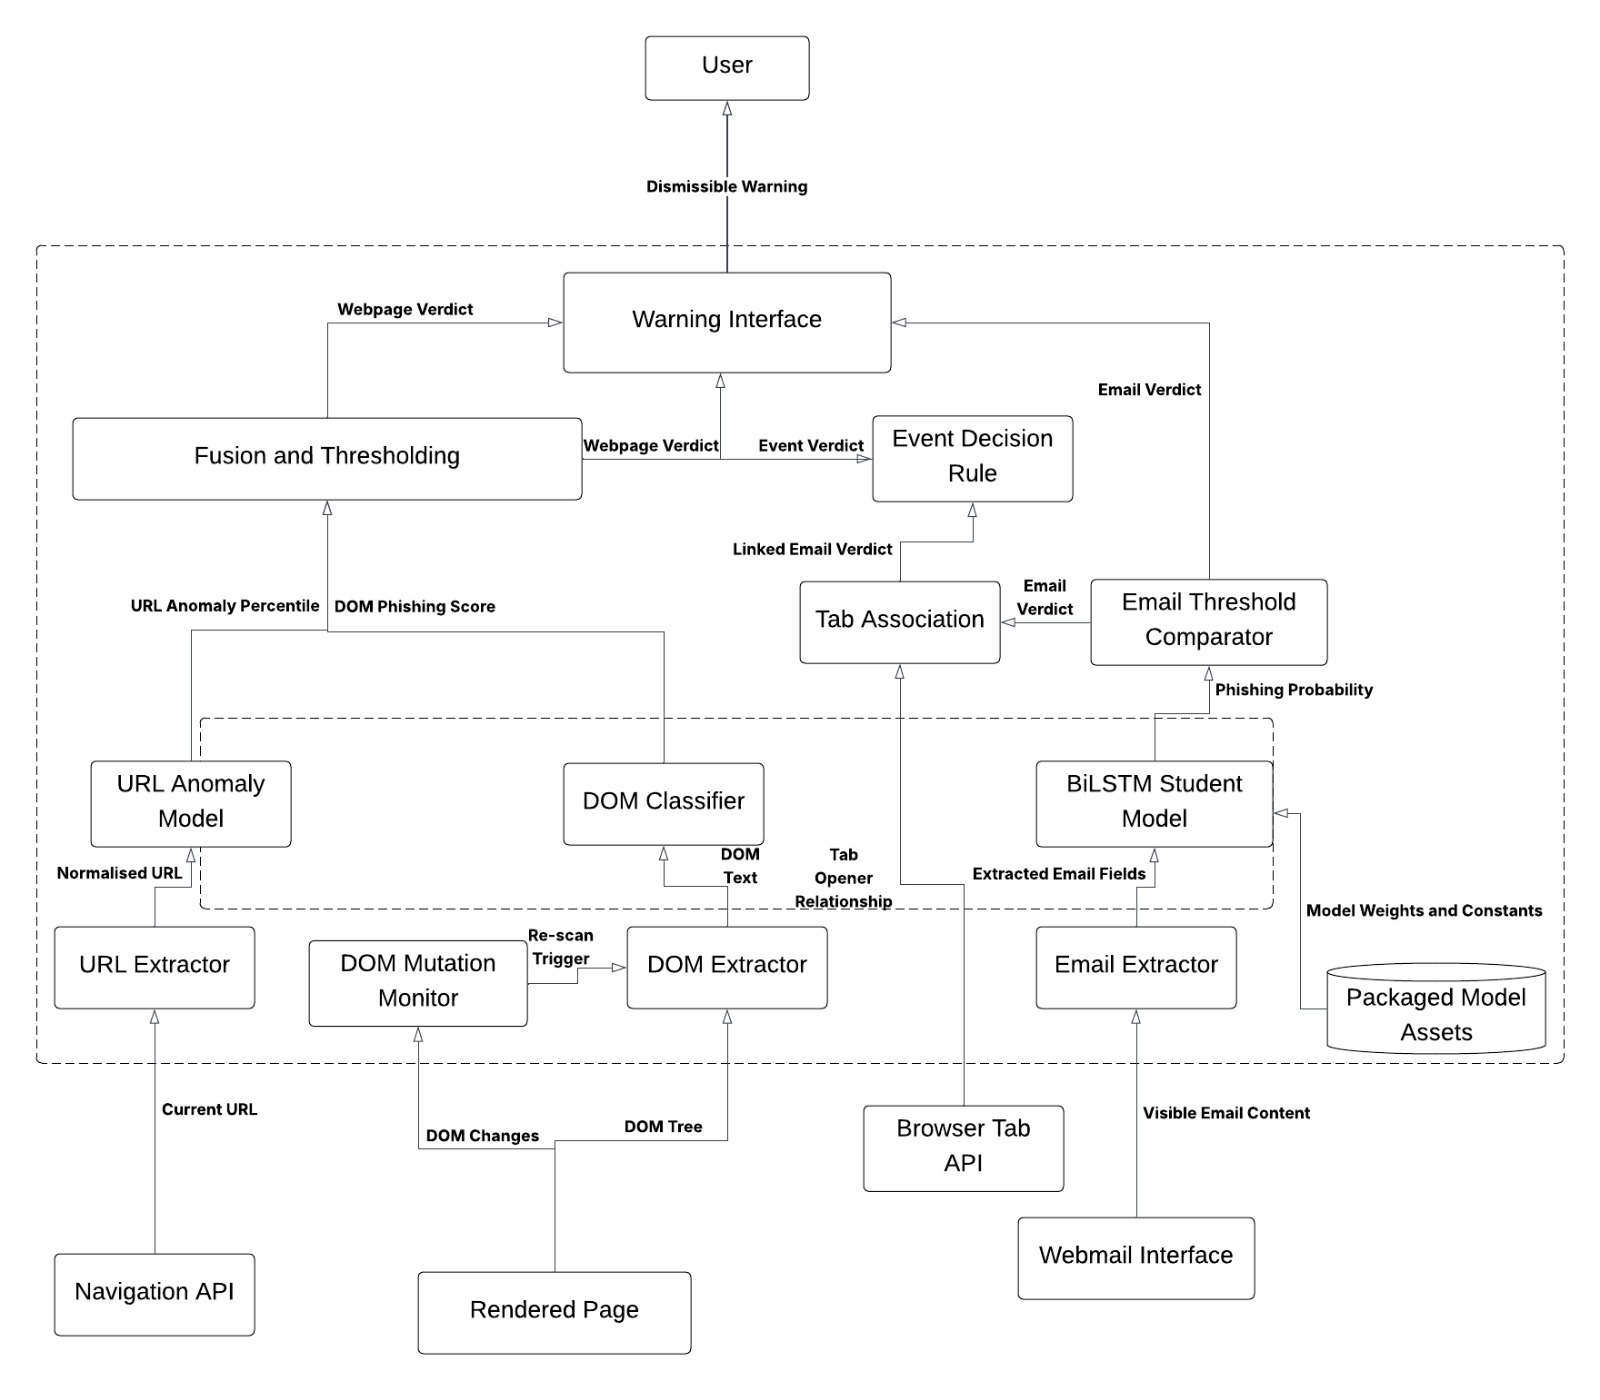
\includegraphics[width=\textwidth]{Figures/fig6.0.png}
    \caption{High-level architecture diagram of PhishHook.}
\end{figure}

The high-level diagram shows the complete system in one view. The URL extractor reads the current URL from the browser navigation API. The DOM extractor reads the rendered DOM. The URL anomaly model and DOM classifier produce two scores, which the fusion and thresholding module combines into a verdict. Email is separately processed and produce its own score which tell email is legitimate or not.

\section{Subsystem Architecture}
\label{sec:design-subsystems}

This section describes the internal architecture of each PhishHook subsystem. Every subsystem is shown by it's own diagram which shows its inputs, internal components, and outputs.

\subsection{URL and DOM Extraction Subsystem}
The URL and DOM extraction subsystem is the first stage of the web pipeline. It takes the current URL from the browser navigation API and reads the DOM tree of the rendered page. The URL is passed through a normalisation stage that removes the fragment, lower-cases the scheme and host, and applies the same routine that was used to prepare the training data. The DOM extractor reads the rendered page and extracts the prioritised fields defined in the preprocessing configuration. An extraction controller runs both extractors together. It outputs the normalised URL and the DOM-derived text, and passes them on to the URL and DOM models. The same extraction code is used offline to prepare training data, so training and deployment inputs match. Structure of this module is shown in Figure~\ref{fig:extraction}.

\begin{figure}[H]
    \centering
    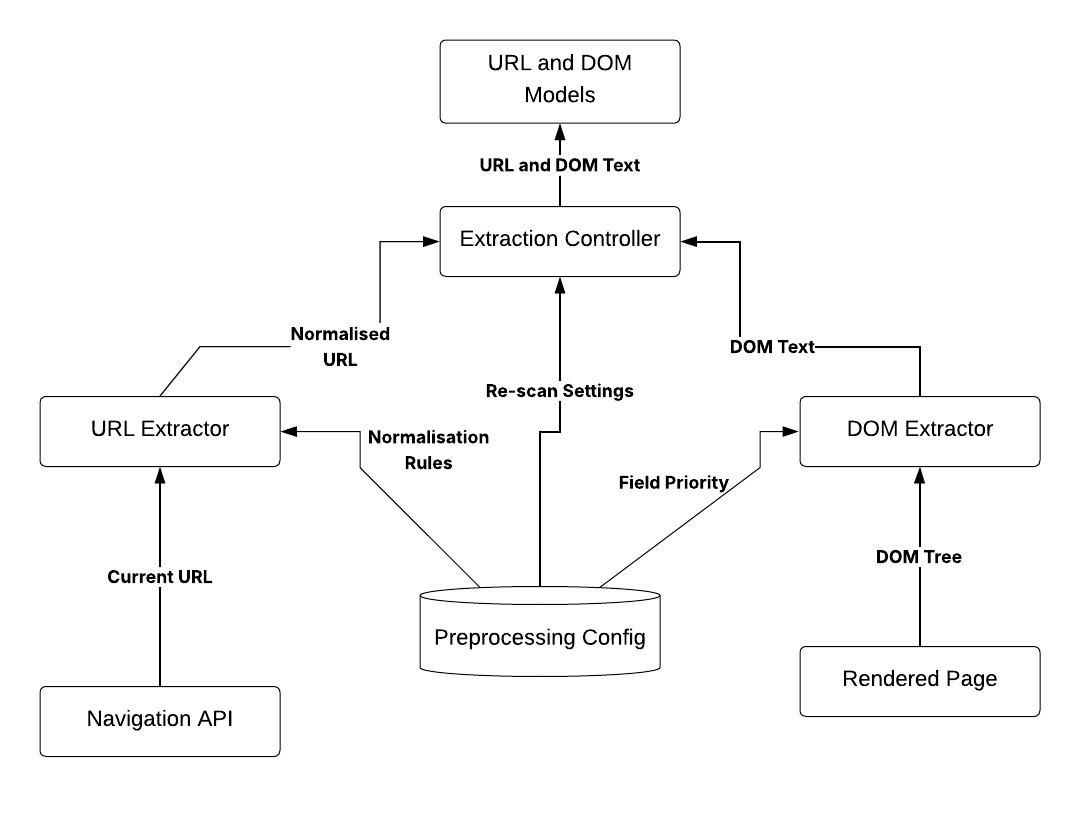
\includegraphics[width=0.85\textwidth]{Figures/fig6.1.png}
    \caption{URL and DOM extraction subsystem.}
    \label{fig:extraction}
\end{figure}

\subsection{Webpage Detection and Score Fusion Subsystem}
The webpage detection and score fusion subsystem combines the outputs of the two web models into a single verdict. The URL anomaly model reads the normalised URL and produces a raw anomaly score, which is converted to a percentile using the frozen benign quantiles shipped with the extension. The DOM classifier reads the DOM-derived text and produces a phishing score. The fusion and thresholding module combines the URL percentile and the DOM phishing score using coefficients and thresholds loaded from the model configuration. The model configuration is stored inside the extension package and is never fetched from a remote server. The result is a webpage verdict that is passed to the warning interface. Structure of this module is shown in Figure~\ref{fig:fusion}.

\begin{figure}[H]
    \centering
    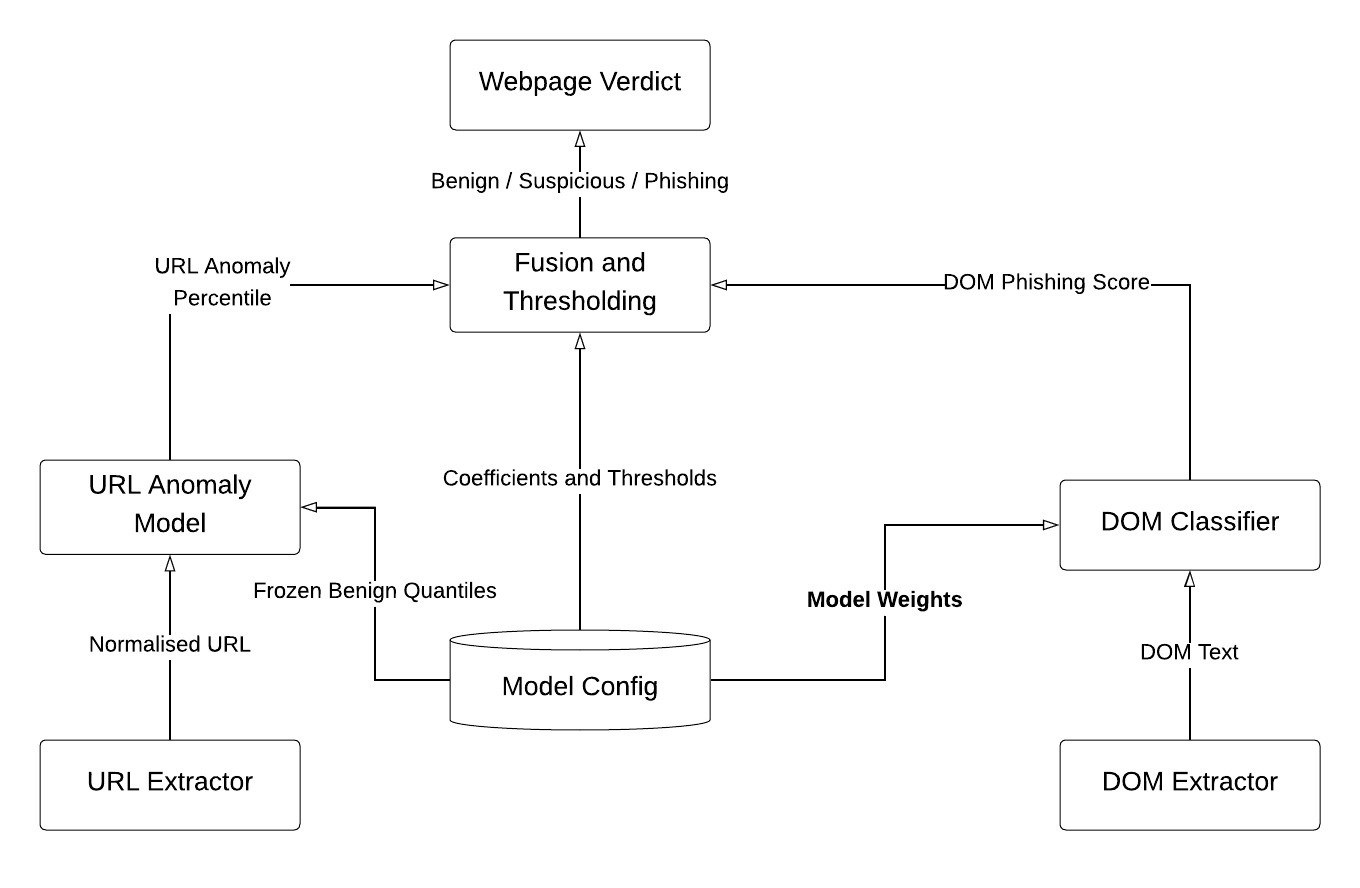
\includegraphics[width=0.85\textwidth]{Figures/fig6.2.png}
    \caption{Webpage detection and score fusion subsystem.}
    \label{fig:fusion}
\end{figure}

\subsection{Email Phishing Detection Subsystem}
The email phishing detection subsystem classifies emails shown in the webmail interface. The email extractor reads visible email content from the webmail interface and produces the extracted email fields, defined in the same way as the training data: subject, visible sender, visible body text, links, and attachment names. A separate adapter is used for each supported webmail client, Gmail and Outlook web, and each one locates the open message before the fields are read. The BiLSTM student model reads these fields and produces a phishing probability, which is then thresholded to produce an email verdict. If an email is flagged as phishing, a dismissible warning banner is shown inside the webmail page. We are also using the unsupervised learning model for the url that present in the email DOM. The student BiLSTM model's weights are loaded from the model configuration inside the extension package, so no remote fetch is required. The MobileBERT teacher is used only during training, so the BiLSTM student is the only email model that ships with the extension. If the webmail DOM cannot be parsed, no verdict is produced rather than a wrong verdict. Structure of this module is shown in Figure~\ref{fig:email}.

\begin{figure}[H]
    \centering
    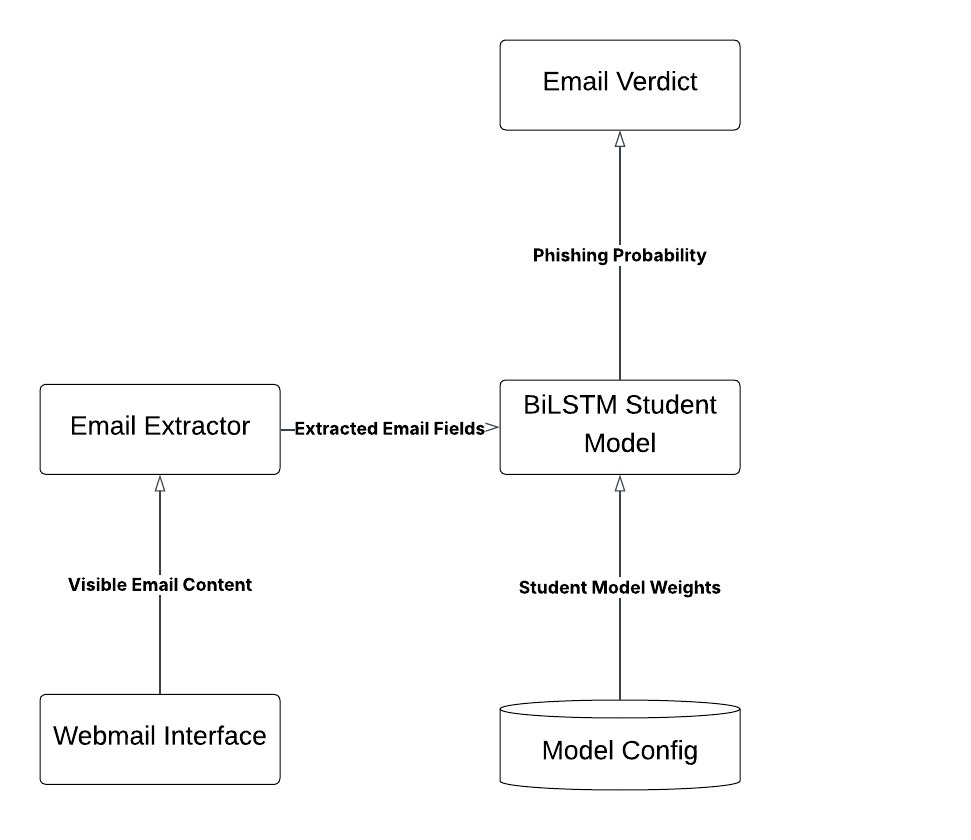
\includegraphics[width=0.85\textwidth]{Figures/fig6.3.png}
    \caption{Email phishing detection subsystem.}
    \label{fig:email}
\end{figure}

\subsection{Dynamic Monitoring and Warning Generation Subsystem}
The dynamic monitoring and warning generation subsystem watches the page for changes after it has loaded and warns the user when a suspicious verdict is produced. The DOM mutation observer watches the rendered page for changes and forwards high-signal changes to the monitoring controller. Not every change is worth a rescan so only the ones that matter for phishing are passed on like a new password field or form, a frame from a new source, a page body that has mostly been rebuilt or a route change inside the page. Everything else is ignored. The monitoring controller uses the window, throttle, and inference cap settings from the monitoring configuration to decide when to trigger a rescan. Re-scans are debounced, which means the controller waits until the page has stopped changing for a short while, and if a newer request arrives while one is waiting, the newer one replaces it. To keep CPU use under control, there is a cool-down between scans and a limit on how many scans a single page can trigger. When a re-scan is required, the controller sends a re-scan request to the detection pipeline and receives an updated verdict. A re-scan also happens when the user submits a form, and if the page has not changed since the last analysis, the cached verdict is reused. When the verdict is suspicious or phishing, the controller sends the verdict to the warning interface, which displays a dismissible warning to the user. This warning is drawn in an interface owned by the extension, so the page cannot touch it, and it does not block the page. The user decides whether to continue. Structure of this module is shown in Figure~\ref{fig:monitoring}.

\begin{figure}[H]
    \centering
    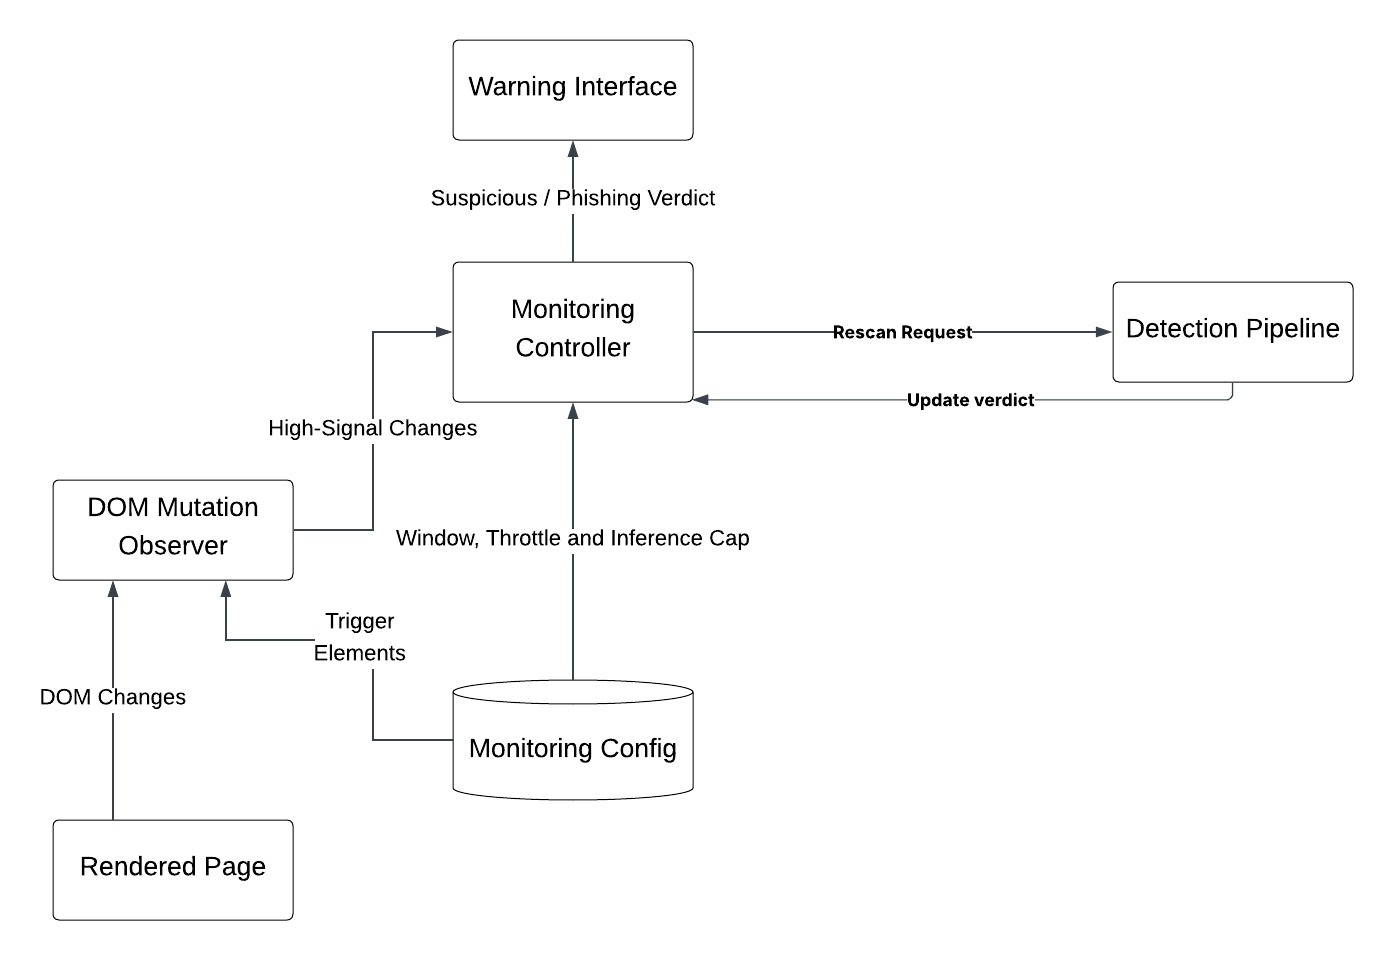
\includegraphics[width=0.90\textwidth]{Figures/fig6.4.png}
    \caption{Dynamic monitoring and warning generation subsystem.}
    \label{fig:monitoring}
\end{figure}

\subsection{Email-to-Web Correlation Subsystem}
The email-to-web correlation subsystem links the verdict on an email to the verdict on the web page it opens. This only applies to mail opened in Gmail or Outlook web, since those are the two webmail clients the email detector supports. When the user clicks a link inside an open webmail message, the browser tab API provides the tab opener relationship to the tab association module. The two verdicts are tied together by how the tab was opened, not by comparing URLs. The extension never opens the link or fetches its destination on its own, and it only notes which tab the user opened. The tab association module links the email verdict, produced by the email detection module to the newly opened web page. This link is short-lived, since it is kept only in the memory of the service worker and is cleared when the worker is terminated. When both the linked email verdict and the webpage verdict are available within the configured time window, the event decision rule combines them into a single event verdict using the rule and time window from the correlation configuration. If one of the two is still missing when the window ends, no combined verdict is produced. The same applies when the user has not granted the webmail permissions, because there is then no email verdict to link and the web page is judged on its own. If no reliable link exists between the two verdicts, the verdicts remain independent and are not combined. In that case each one is still handled on its own, so a warning is not lost just because the link could not be made. The event verdict is passed to the warning interface and shown to the user. None of this is saved to disk or sent anywhere, which keeps it in line with the local-only design of the rest of the extension. Structure of this module is shown in Figure~\ref{fig:correlation}.

\begin{figure}[H]
    \centering
    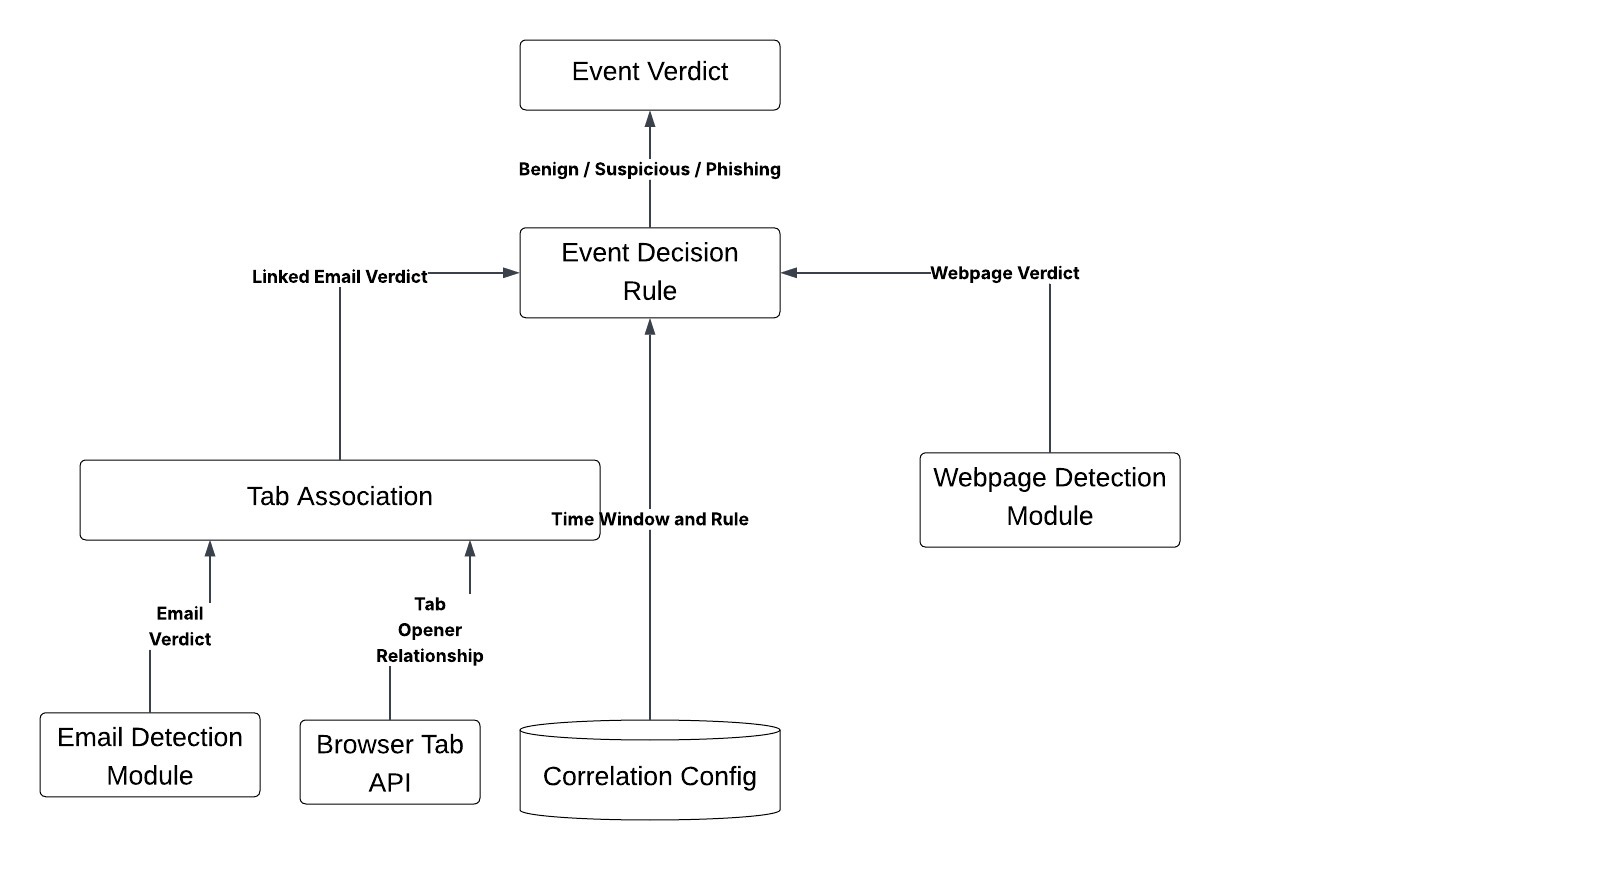
\includegraphics[width=0.95\textwidth]{Figures/fig6.5.png}
    \caption{Email-to-web correlation subsystem.}
    \label{fig:correlation}
\end{figure}

\section{Architectural Strategies}
\label{sec:design-strategies}
The architectural strategies that we will be using for the PhishHook system are given below.

\subsection{Tools and Software}
The extension will be developed using TypeScript and JavaScript, bundled with esbuild. The user interface will use plain HTML and CSS, and the extension will run on Chromium-based browsers using Manifest V3. Model inference inside the browser will use ONNX Runtime Web running through WebAssembly in an offscreen document. Model training and export will be done in Python using PyTorch and ONNX. The URL anomaly module will be implemented with scikit-learn for Isolation Forest and a convolutional autoencoder in PyTorch. The DOM classifier will use MobileBERT. The fusion model will be implemented as a two-input logistic regression. The email student will be a small BiLSTM exported to ONNX. For the code version will use Github and for the model versioning and for test results we use DagsHub and for the dataset storage we use DVC and for the system diagrams use Draw.io and for the GUI prototype use figma. Python is used for training the models, exporting them to ONNX, and running the parity tests that check the browser's output against the original models.

\subsection{Client-Side Extension Model}
PhishHook runs entirely on the client side. There's nothing on the server, no backend, no cloud inference, it's just a browser extension. The extension has 4 components. The URL is extracted by a content script, the rendered DOM is extracted, a service worker coordinates the analysis, and a popup displays the current verdict, which is obtained from running the ONNX models in WebAssembly components within an offscreen document. Content script communicates with the service worker using message passing, and service worker communicates with the offscreen document using the offscreen document API. Messages are sent out asynchronously so the page is not blocked. No data is transmitted from the user's device.

\subsection{Local Data Handling}
This extension do not use any database. There is no permanent storage on the client device and also nothing is store in the client disk or any server because of client privacy.  Page text, email text, and user identifiers are processed in memory only and discarded once inference is complete. Verdicts and diagnostic counters, when they are needed for event correlation during a session, are held in memory only and are not retained after the browser session ends. This is consistent with the privacy requirement that nothing is stored and nothing is transmitted. If any short-lived state is needed for correlation across tabs, it is kept in the service worker's in-memory store and cleared when the worker is terminated.

\subsection{Interface Paradigms}
The interface is kept minimal for not obscuring the regular browsing experience. Each warning is brief, clearly states the problem and can be ignored with one click. A suspicious page and a phishing page get different warnings, so the user can tell how serious the problem is without reading much. For email the warning appears inside the Gmail or Outlook page itself, so the user does not have to leave the message to see it. Warnings are either drawn in an extension owned overlay or in a closed shadow root, so no scripts on the page can read, style or modify warnings. The warning shown when someone tries to submit a form on a flagged page is worded more strongly than the banner at the top since that is the moment credentials are about to be handed over. The popup simply displays the status of the extension and the verdict of the current page and nothing else.

\section{Domain Model / Class Diagram}
\label{sec:domain-model}
Following is the model diagram of the project PhishHook. The diagram shows the two detection surfaces, the web pipeline on top and the email pipeline on the bottom, and how the models and the fusion step are connected.

\begin{figure}[!ht]
    \centering
    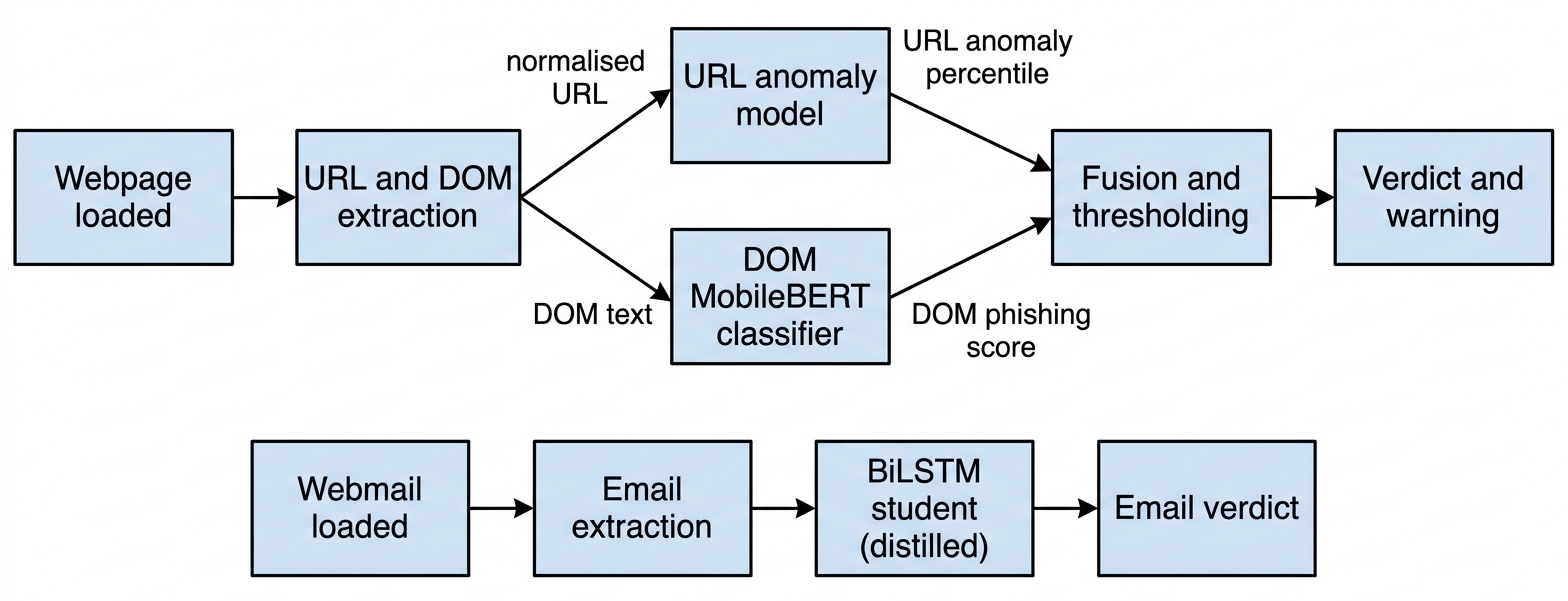
\includegraphics[width=\textwidth]{Figures/model_diagram.png}
    \caption{Model diagram of the PhishHook system.}
    \label{fig:model-diagram}
\end{figure}

The web pipeline begins with the loaded webpage. The URL and DOM extraction step produces a normalised URL and a parsed DOM text. The page URL is left out of the DOM text, so each model only sees its own input. The URL anomaly model and the DOM MobileBERT classifier each produce a score. The DOM score comes from the int8 quantised MobileBERT and is calibrated after quantisation, since quantisation changes the raw scores. The URL score is first converted into a percentile rank using the benign quantiles that ship with the extension, so it sits on a scale comparable to the DOM score. The fusion and thresholding step combines the two scores and produces the verdict that drives the warning interface. The fused score is compared against fixed thresholds, which sort the page into one of three verdicts: benign, suspicious, or phishing. The email pipeline begins with the loaded webmail page. The email extraction step produces the visible email fields, and the distilled BiLSTM student produces the email verdict. The two pipelines run separately. They meet only in the email-to-web correlation step, which combines an email verdict with the verdict of the page opened from it.


\section{Sequence Diagrams}
\label{sec:sequence-diagrams}
In this section, the sequence diagrams for the main system components are shown along with a description of their working.

\subsection{PhishHook System}
This diagram represents the overall working of the system and shows the sequence of actions triggered when a user loads a web page. The content script extracts the URL and the DOM-derived text, the service worker coordinates the analysis, and the offscreen document runs the URL, DOM, and fusion models.

\begin{figure}[H]
\centering
\begin{tikzpicture}[
    every node/.style={font=\footnotesize, color=black},
    lifeline/.style={draw, dashed, color=black},
    msg/.style={-{Latex}, thick, color=black},
    box/.style={draw, rectangle, minimum width=2.6cm, minimum height=0.8cm, align=center, fill=white, text=black}
]
\node[box] (user) at (0,0) {User};
\node[box] (cs) at (3.2,0) {Content script};
\node[box] (sw) at (6.4,0) {Service worker};
\node[box] (od) at (9.6,0) {Offscreen document};
\draw[lifeline] (user.south) -- ++(0,-8);
\draw[lifeline] (cs.south) -- ++(0,-8);
\draw[lifeline] (sw.south) -- ++(0,-8);
\draw[lifeline] (od.south) -- ++(0,-8);
\draw[msg] (0,-0.9) -- (3.2,-0.9) node[midway,above,font=\scriptsize,color=black]{load page};
\draw[msg] (3.2,-1.8) -- (6.4,-1.8) node[midway,above,font=\scriptsize,color=black]{URL and DOM text};
\draw[msg] (6.4,-2.7) -- (9.6,-2.7) node[midway,above,font=\scriptsize,color=black]{run models};
\draw[msg] (9.6,-3.6) -- (6.4,-3.6) node[midway,above,font=\scriptsize,color=black]{fused score};
\draw[msg] (6.4,-4.5) -- (3.2,-4.5) node[midway,above,font=\scriptsize,color=black]{verdict};
\draw[msg] (3.2,-5.4) -- (0,-5.4) node[midway,above,font=\scriptsize,color=black]{show warning if phishing};
\end{tikzpicture}
\caption{PhishHook system design sequence diagram.}
\label{fig:seq-system}
\end{figure}

\subsection{DOM Parser}
The following diagram represents the working of the DOM parser, initiated once the page has finished loading and its DOM has settled. The parser traverses the rendered DOM, collects the seven element groups, normalises the text, and serialises them in priority order.

\begin{figure}[H]
\centering
\begin{tikzpicture}[
    every node/.style={font=\footnotesize, color=black},
    lifeline/.style={draw, dashed, color=black},
    msg/.style={-{Latex}, thick, color=black},
    box/.style={draw, rectangle, minimum width=2.6cm, minimum height=0.8cm, align=center, fill=white, text=black}
]
\node[box] (page) at (0,0) {Rendered DOM};
\node[box] (parser) at (3.4,0) {DOM parser};
\node[box] (groups) at (6.8,0) {Element groups};
\node[box] (serial) at (10.2,0) {Serialised text};
\draw[lifeline] (page.south) -- ++(0,-6);
\draw[lifeline] (parser.south) -- ++(0,-6);
\draw[lifeline] (groups.south) -- ++(0,-6);
\draw[lifeline] (serial.south) -- ++(0,-6);
\draw[msg] (0,-0.9) -- (3.4,-0.9) node[midway,above,font=\scriptsize,color=black]{traverse};
\draw[msg] (3.4,-3.4) -- (6.8,-3.4) node[midway,above,font=\scriptsize,color=black]{collect seven groups};
\draw[msg] (6.8,-5.8) -- (10.2,-5.8) node[midway,above,font=\scriptsize,color=black]{serialise in priority order};
\end{tikzpicture}
\caption{DOM parser design sequence diagram.}
\label{fig:seq-dom}
\end{figure}

\subsection{URL Anomaly Module}
The diagram illustrates the URL anomaly module's function. When a page loads, the URL is normalised and scored by the deployed model, and its percentile rank is computed from the shipped benign quantiles.

\begin{figure}[H]
\centering
\begin{tikzpicture}[
    every node/.style={font=\footnotesize, color=black},
    lifeline/.style={draw, dashed, color=black},
    msg/.style={-{Latex}, thick, color=black},
    box/.style={draw, rectangle, minimum width=2.6cm, minimum height=0.8cm, align=center, fill=white, text=black}
]
\node[box] (url) at (0,0) {URL string};
\node[box] (norm) at (3.4,0) {URL normaliser};
\node[box] (model) at (6.8,0) {Deployed URL model};
\node[box] (pct) at (10.2,0) {Percentile rank};
\draw[lifeline] (url.south) -- ++(0,-5);
\draw[lifeline] (norm.south) -- ++(0,-5);
\draw[lifeline] (model.south) -- ++(0,-5);
\draw[lifeline] (pct.south) -- ++(0,-5);
\draw[msg] (0,-0.9) -- (3.4,-0.9) node[midway,above,font=\scriptsize,color=black]{normalise};
\draw[msg] (3.4,-1.9) -- (6.8,-1.9) node[midway,above,font=\scriptsize,color=black]{score URL};
\draw[msg] (6.8,-4.3) -- (10.2,-4.3) node[midway,above,font=\scriptsize,color=black]{map against benign quantiles};
\end{tikzpicture}
\caption{URL anomaly module design sequence diagram.}
\label{fig:seq-url}
\end{figure}

\subsection{Email Classification}
The working of the email classification module is represented in the diagram below. When an email is opened, the parser collects only the parts the user can see, and the distilled BiLSTM student classifies them to decide whether the email is phishing.

\begin{figure}[H]
\centering
\begin{tikzpicture}[
    every node/.style={font=\footnotesize, color=black},
    lifeline/.style={draw, dashed, color=black},
    msg/.style={-{Latex}, thick, color=black},
    box/.style={draw, rectangle, minimum width=2.6cm, minimum height=0.8cm, align=center, fill=white, text=black}
]
\node[box] (mail) at (0,0) {Webmail page};
\node[box] (parse) at (3.4,0) {Email parser};
\node[box] (student) at (6.8,0) {BiLSTM student};
\node[box] (verdict) at (10.2,0) {Email verdict};
\draw[lifeline] (mail.south) -- ++(0,-5);
\draw[lifeline] (parse.south) -- ++(0,-5);
\draw[lifeline] (student.south) -- ++(0,-5);
\draw[lifeline] (verdict.south) -- ++(0,-5);
\draw[msg] (0,-0.9) -- (3.4,-0.9) node[midway,above,font=\scriptsize,color=black]{open message};
\draw[msg] (3.4,-1.9) -- (6.8,-1.9) node[midway,above,font=\scriptsize,color=black]{subject, sender, body, links};
\draw[msg] (6.8,-4.3) -- (10.2,-4.3) node[midway,above,font=\scriptsize,color=black]{probability and warning};
\end{tikzpicture}
\caption{Email classification design sequence diagram.}
\label{fig:seq-email}
\end{figure}


\section{Policies and Tactics}
\label{sec:policies}
In the following section, we will delve into specific design policies and tactics employed in the development of the PhishHook system. These decisions are carefully crafted to impact the finer details of the system, focusing on the interface and implementation aspects. Unlike architectural decisions that shape the overall organisation of the system, these policies and tactics influence the intricacies of module implementation. Each of these choices is linked back to a requirement in Chapter 4, so it can be checked against the system later. Key considerations discussed here include:

\begin{enumerate}
    \item Selection of model for the URL anomaly module.
    \item Algorithm selection for the DOM classifier and the fusion model.
    \item Testing strategy.
    \item Coding guidelines.
    \item Model packaging and update mechanism.
    \item Plans for ensuring requirements traceability.
\end{enumerate}

\subsection{Algorithm Selection for the URL Anomaly Module}
The URL anomaly module is deployed as either a character-level convolutional autoencoder, Kmean or an Isolation Forest on engineered lexical features. The choice between the three is made by a pre-registered rule on validation data, confirmed on the source-disjoint and temporal test sets. A K-Means distance baseline and a supervised MobileBERT on URL strings are compared offline only to provide reference points. The unsupervised nature of the deployed model is deliberate it reflects the observation that labelled phishing URLs are scarce and quickly go stale. The alternative of using only a supervised URL model was considered and rejected because it would duplicate the signals captured by the DOM classifier and would not generalise as well under temporal shift.

\subsection{Algorithm Selection for the DOM Classifier and the Fusion Model}
The DOM classifier uses MobileBERT fine-tuned on the serialised DOM text, exported to int8 ONNX. LightGBM on engineered features are compared offline only. The choice of MobileBERT is driven by its combination of accuracy and small size relative to full BERT models, and by the fact that a quantised version fits within the extension's memory and latency budget. The fusion model uses an L2-regularised logistic regression with two inputs. A tree-based fusion model was considered and rejected because it would overfit the limited calibration and fusion data and would add complexity without a demonstrated benefit.

\subsection{Testing Strategy}
Testing is divided into extension test and models test. Extension is tested using unit tests, integration tests and scenario tests in a real Chrome browser. The models are evaluated on the following metrics from the methodology chapter: true-positive rate at fixed false-positive rates, precision--recall AUC, calibration error, model size, and F1 score. All comparisons of two models are accompanied by bootstrap confidence intervals and McNemar's test, no difference is declared on the basis of a single score. The final numbers are only derived from test sets that were not used to select a model, a hyperparameter or a threshold, such as the small set of pages collected during real browsing and the source-disjoint set.

\subsection{Coding Guidelines}
The TypeScript code is written according to the official TypeScript style guide and the Python code is written according to the PEP~8. These conventions help the team apply the same code to work on the system and make it easier to maintain in the future.

\subsection{Model Packaging and Update Mechanism}
No remote code is ever downloaded, all models are embedded in the extension and retrieved from local storage via the extension's own resource API. The model updates are sent as they are and this is similar to the Manifest V3 rule against running code remotely. Every model file is accompanied by its preprocessor code and hence a new version of a model always comes with the tokeniser, parser and fusion constants with which it was trained. That way, the deployed behaviour matches what was trained.

\subsection{Plans for Ensuring Requirements Traceability}
In the case of PhishHook, the requirements are still followed throughout the whole project lifecycle, although it is a research project. Each component, feature and function is associated with a requirement from the Software Requirement Specifications chapter and if applicable, the associated research question. A traceability matrix will be created to map the mapping of each functional requirement to the appropriate module, test case, and section of the report. This ensures the implementation is in accordance with the requirements and facilitates easy audit.

\section{Conclusion}
\label{sec:design-conclusion}
In this chapter, the high level and low level design of PhishHook was presented. The architectural strategies, class model and sequence diagrams demonstrate how the extension is designed, and how data flows between the components and between the detection modules. The policies and tactics state the algorithm options, testing approach, coding requirements, packaging guidelines, and traceability plan the implementation will adhere to. These combine to form the foundation of PhishHook.










\chapter{Implementation and Test Cases}
\label{ch:implementation}
This chapter describes what has been built for PhishHook so far and how it was checked. The work completed to date is on the model side. It consists of three experiment pipelines that prepare data, train or fit a detector, and measure how it behaves: a supervised MobileBERT classifier for the DOM of web pages, an email detector with a MobileBERT teacher and a BiLSTM student, and an unsupervised anomaly detector for URLs. Each pipeline is a set of Python notebooks and helper scripts that ran on Google Colab or Kaggle. The extension interface that will call these models is planned for FYP-2 and is not part of this chapter. 
Section~\ref{sec:impl-details} describes the platform and the implemented modules. Section~\ref{sec:test-design} lists the checks that were run, with the output each one produced, and Section~\ref{sec:test-metrics} counts how many of them passed. The design that these modules follow is given in Sections~\ref{sec:url-module}, \ref{sec:dom-module} and~\ref{sec:email}, and the measured results are reported in Chapter~\ref{ch:results}. 

\section{Implementation Details}
\label{sec:impl-details}
The implementation follows the three parts used in the rest of the report. Part 1 covers the web DOM, Part 2 covers email, and Part 3 covers URLs. The parts use different datasets and different splits, so their numbers are never compared with each other. They do share some habits. Every split uses a fixed random seed, thresholds are chosen on validation data wherever the notebook allows it, and every notebook writes its outputs to disk so that a run can be repeated or resumed. This section lists the platform first and then each implemented module in the order in which the modules are used.

\subsection{Platform Used}
\label{sec:impl-platform}
The DOM and email experiments ran on Google Colab with a Tesla T4 graphics processing unit (GPU). The URL experiments ran on Kaggle and use scikit-learn models, which do not need a GPU. The Colab notebooks mount Google Drive and write every result to a folder there, so a disconnected runtime loses only the run that was in progress. Table~\ref{tab:platform} gives the environment of each part with the versions that the notebooks printed. A version that is missing from the table was not printed by the notebook.

The data and the pretrained model come from public sources. The DOM data are the parsed pages of the PhishLang repository on GitHub \cite{phishlang2026}, which stores them as a split zip archive and derives them from PhishPedia \cite{phishpedia2021}. The MobileBERT weights are the \texttt{google/\allowbreak mobilebert-uncased} checkpoint from Hugging Face. The URL data are the PhiUSIIL phishing URL dataset, read from a Kaggle input folder as one comma-separated values (CSV) file, and the email data are the MeAJOR corpus \cite{meajor2025}. We stuck to public datasets because they let other researchers reproduce our exact numbers.

\begin{table}[H]
	\centering
	\caption{Platform and versions for each part of the implementation.}
	\label{tab:platform}
	\small
	\begin{tabularx}{\textwidth}{|>{\raggedright\arraybackslash}p{2.2cm}|>{\raggedright\arraybackslash}p{2.6cm}|>{\raggedright\arraybackslash}p{2.6cm}|>{\raggedright\arraybackslash}X|}
		\hline
		\textbf{Part} & \textbf{Platform} & \textbf{Hardware} & \textbf{Versions} \\
		\hline
		Web DOM & Google Colab & Tesla T4 GPU & PyTorch 2.14.1+cu130, Python 3.13.16  \\
		\hline
		Email & Google Colab & Tesla T4 GPU & PyTorch 2.14.1+cu130, transformers 5.22.1, Python 3.13.16 (recorded in \texttt{exp1\_metrics.json}) \\
		\hline
		URL & Kaggle & GPU T4x2 & PyTorch 2.14.1, numpy 1.26.4, pandas 2.2.3, scikit-learn 1.5.2, matplotlib 3.9.2, joblib==1.4.2 \\
		\hline
	\end{tabularx}
\end{table}

\subsection{Implemented Modules}
\label{sec:impl-modules}
Nine modules make up the code written so far: five for the DOM part, two for email and two for URLs. For each module the text below gives its purpose, its input and output, and the steps it follows. The steps describe what the code does and not how the Python is laid out. Abbreviations that are used for the first time in this chapter are defined where they appear.

\subsubsection{DOM Data Discovery and Parsing}
\label{sec:impl-dom-data}
The PhishLang repository ships its parsed pages as a split zip archive. The notebook clones the repository, joins the parts, and extracts one folder of phishing pages and one folder of benign pages. Each page is a text file made of records written as a tag followed by a braced list of fields in JavaScript Object Notation (JSON) style, for example a \texttt{TITLE} record with a text field or an \texttt{INPUT} record with type, name and placeholder fields. The text is already lower-cased, so an upper-case tag followed by a colon and an opening brace marks the start of a record. These files were produced by the PhishLang parser and not by the PhishHook parser of Section~\ref{sec:dom-parsing}. Reading them showed three quirks of that parser: every \texttt{META} record holds the placeholder \texttt{<EMPTY>}, many \texttt{SCRIPT} records are empty, and a \texttt{UL} record repeats the text of the \texttt{LI} records that follow it. The input of this module is the repository archive, and its output is a sorted list of 52,659 labelled page files.
\begin{itemize}
	\item The repository is cloned and the zip parts of the parsed data are joined into one archive.
	\item The phishing archive and the benign archive are extracted into two folders.
	\item Every \texttt{.txt} file in both folders is listed in sorted order, which fixes the page order, and is labelled 1 for phishing or 0 for benign.
	\item The counts are compared with the expected 29,048 phishing and 23,611 benign files, and the run stops if they differ.
	\item The first 20,000 characters of each page are read, and records are separated at every upper-case tag that is followed by a colon and an opening brace.
\end{itemize}

\subsubsection{Corrected MobileBERT Trainer}
\label{sec:impl-trainer}
The original PhishLang training script has three faults that matter for the experiments. Its split picks positions in the unsplit data with indices taken from the split data, which can let pages move between the training and test sets. It keeps about 3.4 GB of page text in memory and then copies it again. And the raw \texttt{[CLS]} output of MobileBERT reached values near $10^{7}$ in a probe, which made the logits explode and overflow in 16-bit arithmetic. The corrected trainer splits on row indices of one list, reads only the start of each page and tokenises once, adds a layer normalisation in front of the classifier, and trains in 32-bit arithmetic. Experiments 1 to 3 call this trainer as a script. Experiments 4 and 5 contain an in-notebook version with the same recipe. The input is the list of labelled files from the previous module, and the output is a saved model, its validation and test logits, and a metrics file.
\begin{itemize}
	\item A stratified split is made on the row indices of one list, first 20\% of the pages for testing and then 10\% of the remaining pages for validation, with seed 42. The script asserts that the three index sets do not overlap and that together they cover all pages.
	\item Every page is tokenised once to 128 tokens with the fast MobileBERT tokenizer, and the ids and attention masks are stored as integer arrays.
	\item The \texttt{google/\allowbreak mobilebert-uncased} model is loaded with a two-class head, and its pooler is replaced by a layer normalisation of the \texttt{[CLS]} vector.
	\item The model is trained in 32-bit arithmetic with micro-batches of 32 pages and four accumulation steps, which gives an effective batch of 128. In the script, weight decay is 0.01 and gradients are clipped at 1.0, and the learning rate is 2e-5 unless an experiment changes it.
	\item After every epoch the model is evaluated on the validation pages, the metrics are appended to a file, and a checkpoint is saved. The checkpoint with the best validation F1 is kept.
	\item The kept checkpoint predicts the validation and test pages, the logits are saved, and the final metrics and the run configuration (arguments, library versions, training time) are written to disk.
\end{itemize}

\subsubsection{DOM Input Transforms}
\label{sec:impl-transforms}
A 128-token window sees only the start of a page, and the start of a long page is often scripts and menu text. The transforms change the text before tokenisation so that the window holds more useful records. They work on text only and never read the label. Three transforms were implemented. The compaction transform removes filler, the reordering transform moves the records that matter for phishing to the front, and the prefix transform adds one line of page-level counts. The input is the page text, and the output is the rewritten text that is passed to the tokeniser.
\begin{itemize}
	\item The page text is split into records at each known tag followed by a colon and an opening brace.
	\item Compaction drops empty records of the types \texttt{META}, \texttt{SCRIPT}, \texttt{P}, \texttt{UL}, \texttt{OL}, \texttt{LI}, \texttt{H1}, \texttt{H2}, \texttt{H3}, \texttt{MAP} and \texttt{AREA}.
	\item Compaction drops a \texttt{UL} or \texttt{OL} record when an \texttt{LI} record follows it, because the \texttt{LI} records repeat its text, and drops an \texttt{LI} record when the next \texttt{LINK} record carries the same text.
	\item Compaction drops any record that is identical to the one before it. The remaining records are joined and the first 6,000 characters are kept, from at most 100,000 characters read.
	\item Reordering is a stable sort that places \texttt{TITLE} records first, then \texttt{FORM}, \texttt{INPUT}, \texttt{CHECKBOX}, \texttt{LABEL}, \texttt{BUTTON} and \texttt{IFRAME} records, and then everything else, with the original order kept inside each group.
	\item The prefix transform counts forms, inputs, password fields, hidden fields, buttons, iframes, scripts, links, external links and empty records over the whole page, reading up to 500,000 characters, and writes one summary line in front of the text.
\end{itemize}
The summary line costs a median of 23 tokens, at most 26, out of the 126 tokens that remain after the two special tokens. The ablation notebook builds six slices of the same text (title and headings, title and forms, everything except body text, body text only, everything except forms, and the full text) and caps each record at 600 characters.

\subsubsection{Evaluation Toolkit}
\label{sec:impl-eval}
All DOM runs are scored with one small toolkit so that the numbers are comparable. The score of a page is the difference between the two logits, and a page is called phishing when the score is above zero. The toolkit reports phishing-class precision, recall and F1, the weighted averages that the PhishLang repository reports, the FPR, the area under the receiver operating characteristic curve (ROC-AUC), and the TPR at 1\% and 0.1\% FPR, read from the ROC curve by interpolation. Uncertainty and significance are handled with resampling and an exact test. The input is a logits file and the labels, and the output is a table of metrics, intervals and test results.
\begin{itemize}
	\item A validation threshold is found by sorting the validation scores of benign pages and taking the score that lets at most the target share of them through as phishing.
	\item A 95\% interval for F1 is taken from 2,000 bootstrap resamples of the test pages (1,000 in the leakage notebook).
	\item The difference in F1 between two variants is computed on the same resamples, which gives a paired interval.
	\item An exact McNemar test is run on the pages that one variant classifies correctly and the other does not.
	\item The expected calibration error (ECE) uses 15 bins, and the Brier score and the negative log-likelihood (NLL) are computed with it. Temperature scaling fits one scalar on the validation logits by one-dimensional minimisation.
	\item Precision at a given base rate is computed from the measured TPR and FPR as $\mathrm{TPR}\cdot\pi / (\mathrm{TPR}\cdot\pi + \mathrm{FPR}\cdot(1-\pi))$, with $\pi = 1/(1+k)$ for one phishing page per $k$ benign pages, for $k$ equal to 100, 1,000 and 10,000.
	\item For variants trained with more than one seed, the mean and standard deviation of F1 are reported, and an ensemble is formed by averaging the logits of the seeds.
\end{itemize}

\subsubsection{Leakage Analysis Tool}
\label{sec:impl-leakage}
The PhishLang data contain many repeated phishing pages, so a random split can put near-copies of a test page into training. The leakage tool measures this and builds a second split in which related pages stay together. It needs only the page texts and labels, and it produces per-class leakage rates and a grouped split of the same proportions as the random one (72/8/20). The grouping key for a phishing page is the brand read from the file name, which is a heuristic, and the key for a benign page is its domain name.
\begin{itemize}
	\item Each non-empty page is given an MD5 hash of its first 20,000 characters and its character count, and pages with equal hashes are counted as exact repeats within their class.
	\item Hashed word 1-gram to 3-gram vectors with 262,144 features, binary values and unit length are built from the first 3,000 characters of each page, and each test page is matched to its most similar training page by cosine similarity.
	\item For each class, the share of test pages with an exact copy, or with a similarity of at least 0.99, 0.95, 0.90 and 0.80, in the training set is reported.
	\item Group keys are built: the text before the plus sign in the file name for phishing pages, and the domain without a leading \texttt{www.} for benign pages.
	\item Groups that contain identical pages are merged with a union-find structure. Content that appears more than 50 times is skipped for merging, so that a generic page cannot join unrelated brands, and 10,446 pages were skipped this way.
	\item The groups of each class are shuffled, sorted by size from large to small, and placed one by one in the split that is furthest below its target share.
	\item The number of groups that appear in two splits is printed, and the target is zero.
	\item The classifier is trained and tested on both the random split and the grouped split.
\end{itemize}

\subsubsection{Email Pipeline}
\label{sec:impl-email}
The email notebook trains the MobileBERT teacher on emails shown in the webmail view of Section~\ref{sec:email-mapping}. The MeAJOR corpus has 108,684 labelled emails. After empty and duplicate texts are removed, 104,427 remain, and no text carries two different labels. The emails are grouped into campaigns, 99,362 groups in all, and each group is placed in one split, so near-identical messages cannot sit on both sides of the train and test boundary. The four splits hold 72,993 training, 10,379 validation, 10,663 calibration and 10,392 test emails, and about 45\% of the test emails are phishing. The input is the corpus, and the output is a metrics file, a per-seed results table, a learning-rate table and a figure with four plots (\texttt{exp1\_plots.png}).
\begin{itemize}
	\item Empty and duplicate email texts are removed, and the number of texts with conflicting labels is counted, which is zero.
	\item Each email is converted into the webmail view and tokenised to 512 tokens. Between 21.2\% and 21.6\% of the emails are truncated in each split.
	\item Campaign groups are built, and whole groups are assigned to the training, validation, calibration and test splits with split seed 2026.
	\item The learning rate is chosen from two candidates, 2e-5 and 3e-5, by the validation PR-AUC of a run with seed 42. The value 3e-5 wins with 0.9986 against 0.9984.
	\item The teacher is trained with seeds 42, 43 and 44 for at most three epochs, with a batch size of 16, a patience of two epochs and 32-bit arithmetic. Training can resume from saved state after a disconnect.
	\item A temperature is fitted for each seed and a decision threshold is chosen without using the test emails. 
	\item The seed with the highest validation PR-AUC, which is seed 44 at 0.9988, is selected for the detailed report, and metrics, confidence intervals and plots are saved.
\end{itemize}
Each seed took between 90.3 and 92.1 minutes to train. The notebook also records that the teacher classifies 99.82\% of its own training emails correctly. This matters for distillation, because soft labels computed on training emails are more confident than the same teacher would be on new emails. 

\subsubsection{Email Distillation Module}
\label{sec:impl-distill}
The distillation module is written, but its full run has not been carried out. It trains a BiLSTM student on the soft labels of the MobileBERT teacher. The student has its own vocabulary and embeddings, so the teacher and student share outputs only. The training loss mixes the usual cross-entropy (CE) on the true labels with a Kullback--Leibler (KL) divergence between the softened outputs of teacher and student:
\begin{equation}
	\mathcal{L} \;=\; (1-\alpha)\,\mathrm{CE}\bigl(y,\,p_s\bigr) \;+\; \alpha\,T^{2}\,\mathrm{KL}\bigl(p_t^{(T)} \,\Vert\, p_s^{(T)}\bigr),
	\label{eq:kd-loss}
\end{equation}
where $\alpha$ weighs the two terms, $T$ is the temperature, $p_s$ and $p_t$ are the student and teacher outputs, and the superscript $(T)$ marks outputs softened with temperature $T$. 
The plan compares two configurations of the student with the same architecture, the same splits and seeds, and the same tuning budget of six runs each. The notebook records only four finished tuning runs for the first configuration (model A in the notebook), no run for the second (model B), and no final seeds. For this reason the report contains no distillation result. The evaluation that is planned for FYP-2 uses the mean and standard deviation over seeds, bootstrap intervals, an exact McNemar test, and the share of the teacher--student gap that distillation closes. 

\subsubsection{URL Feature Extraction and Selection}
\label{sec:impl-url-features}
The URL part works on the raw URL string only. The PhiUSIIL file has 235,795 rows, of which 425 are duplicate URLs, which leaves 235,370 unique URLs (134,850 benign and 100,520 phishing). Two feature sets were built. Experiment 1 follows a reference paper and extracts 99 features: 17 symbol counts for each of five URL parts (the whole URL, the domain, the directory, the file and the parameters) and 14 structural features. Experiments 2 to 4 use a set of 35 lexical features, found by dropping 10 zero-importance features from 45. These include character counts, digit ratio, entropy of the URL and of the host name, word-length statistics, and four distances between the character distribution of a URL and a reference benign distribution. The reference distribution is the mean over 25,000 benign training URLs, so no test URL influences it. The input is the CSV file, and the output is one feature table per experiment and the selected feature lists.
\begin{itemize}
	\item The URL column and the label are read, and duplicate URLs are removed.
	\item Features are extracted from each URL string. For reference Paper this takes 17.8 seconds for all URLs, and for the 35-feature set it takes 51.7 seconds.
	\item The data are split with a stratified split and seed 42, 80/20 in Experiments 1 to 3 and 70/30 in Experiment 4. A further 15\% of the training pool is held out as validation.
	\item In Experiment 1, 24 constant columns are removed, which leaves 75, and 12 columns with an absolute correlation above 0.80 are dropped, which leaves 63. Two multilayer perceptrons, one with layers of 128 and 64 units and one with 128, 64 and 32 units, are fitted on the training part, and features are ranked by permutation importance on the validation part with five repeats. The top 20 and the top 14 features are kept.
	\item In Experiment 2, recursive feature elimination (RFE) with a decision tree of depth 12 and a Random Forest with 60 trees each pick 20 features, and 16 of the 20 are shared.
	\item In Experiment 3, five selectors pick 20 features each: chi-square, mutual information on the first 50,000 training rows, an L1-penalised logistic regression, a Random Forest with 50 trees, and RFE with a decision tree. The Random Forest and RFE lists contain the same 20 features in a different order, which is why their results are identical.
\end{itemize}
The scheme of a URL is not excluded from these features. In Experiment 1 the feature \texttt{tls\_ssl\_certificate} is one when the scheme is \texttt{https}, and it ranks first by permutation importance. In Experiments 2 to 4 the feature \texttt{https\_token} is one when \texttt{https} appears in the host name or the path or when the scheme is \texttt{https}. Section~\ref{sec:url-parsing} states that the scheme is left out of the feature set, so the code and the design disagree on this point. It is listed as a failed check in Section~\ref{sec:test-url}.

\subsubsection{Unsupervised URL Experiments}
\label{sec:impl-url-experiments}
Four experiments fit an unsupervised detector on benign URLs and test it on a mix of benign and phishing URLs. They differ in the split, the features and the detector, as Table~\ref{tab:url-experiments} shows, and they were not designed as one controlled comparison. Each experiment is one code cell in the Kaggle notebook. The input is a feature table from the previous module, and the output is a table of metrics at three operating points, confusion matrices, and a figure. The detectors are K-Means with the distance to the nearest of 10 centroids as the anomaly score, and an Isolation Forest whose score is the negated output of \texttt{score\_samples}. No other detector is used in this part.
\begin{itemize}
	\item The features are standardised with a scaler fitted on the benign fit set only.
	\item The detector is fitted on benign URLs only. K-Means uses 10 clusters, a batch size of 2,048, 10 initialisations and seed 42. The Isolation Forest uses 150 trees, 2,048 samples per tree, automatic contamination and seed 42.
	\item Benign validation URLs and test URLs are scored, so that a higher score means a more unusual URL.
	\item Two thresholds are set at the 99th and 95th percentile of the benign validation scores, which targets an FPR of 1\% and 5\%.
	\item A third threshold maximises the difference between TPR and FPR on the ROC curve (Youden's J statistic). Experiments 1 and 2 compute it on the validation split, and Experiments 3 and 4 compute it on the test set.
	\item The thresholds are applied to the test set, and accuracy, precision, recall, FPR, F1 and the confusion matrices are written out. The Isolation Forest experiment also reports PR-AUC and the time to score one URL, which was 0.0085 ms for the RFE feature set as printed. The timing covers scoring the scaled test matrix and excludes feature extraction.
\end{itemize}

\begin{table}[H]
	\centering
	\caption{Setup of the four unsupervised URL experiments.}
	\label{tab:url-experiments}
	\small
	\begin{tabularx}{\textwidth}{|c|c|>{\raggedright\arraybackslash}X|>{\raggedright\arraybackslash}p{2.6cm}|c|>{\raggedright\arraybackslash}p{2.9cm}|}
		\hline
		\textbf{No.} & \textbf{Split} & \textbf{Features} & \textbf{Detector} & \textbf{Benign fit set} & \textbf{Youden threshold} \\
		\hline
		1 & 80/20 & Top 20 and top 14 of 63 candidates from 99 & K-Means & 91,698 & Validation split \\
		\hline
		2 & 80/20 & RFE top 20 and Random Forest top 20, from 35 & Isolation Forest & 91,698 & Validation split \\
		\hline
		3 & 80/20 & Top 20 from each of five selectors, from 35 & K-Means & 91,698 & Test set \\
		\hline
		4 & 70/30 & All 35 features & K-Means & 80,235 & Test set \\
		\hline
	\end{tabularx}
\end{table}

\subsection{Summary}
\label{sec:impl-summary}
The DOM part is complete as an experiment pipeline. It has a corrected trainer, three input transforms, an evaluation toolkit and a leakage tool, and it has produced results for five experiments. The email part has a finished teacher and a written but unexecuted distillation module. The URL part has four unsupervised experiments, all fitted on benign URLs only. Several items are not done. INT8 quantisation of the DOM model has not been run, the distillation run is incomplete, browser latency and memory have not been measured, and the extension interface is planned for FYP-2. The code also has two known departures from the design in Chapter~\ref{ch:methodology}: the URL features include the scheme, and the Youden thresholds of Experiments 3 and 4 were set on the test set. 

\section{Test Case Design and Description}
\label{sec:test-design}
The project has no separate test harness. The checks listed here are assertions, printed counts and comparisons that were run inside the notebooks, and each row of the tables gives the output that the notebook printed or the file that it saved. A case is marked Passed when its criterion was met, Failed when the criterion was not met and the limitation is recorded in this report, and Not executed when the run did not take place. The tables follow the layout of the report template, with an identifier, an objective, the module under test, the steps, the result and a status. The environment is the same for all cases of a part and is given in the text above each table: Google Colab with a Tesla T4 GPU for the DOM and email parts, and Kaggle for the URL part. No usability study was carried out, and no availability or user-count measure exists, so none is reported. The cases are grouped by part, because the three parts use different data and are never compared with each other.


\subsection{Test Cases for the Web DOM Part}
\label{sec:test-dom}
The DOM checks ran in the five Colab notebooks of Part 1. The first group, in Table~\ref{tab:tc-dom-data}, covers the data and the splits. The second group, in Table~\ref{tab:tc-dom-train}, covers the input transforms and the training runs. We kept these checks simple to make debugging easier later on. Since we didn't build a separate test harness, every check here is just an assertion or a printed count that runs automatically inside the notebook. This means anyone can re-run a cell and see the exact same output. One case failed, and it concerns an ablation variant and not the code: the body-only input is empty for a third of the phishing pages, so a model could use emptiness as a shortcut. If we had ignored this, the ablation results would have been misleading. We decided to keep the variant and just report it with that caveat so the limitation is clear to anyone reading the results. Looking back, a better fix would have been to exclude those empty pages from the body-only test, but that would have changed the dataset for everyone else. So we left it in and just made a mental note for the next phase. This is a common issue when you are training multiple models on the same data. Changing one thing often breaks another. We chose transparency over a perfect score here. The failed check stays in the table so that future students know exactly what went wrong and why we didn't sweep it under the rug.

\begin{table}[H]
	\centering
	\caption{Test cases for the web DOM part: data and split checks.}
	\label{tab:tc-dom-data}
	\footnotesize
	\resizebox{\textwidth}{!}{%
		\begin{tabularx}{\textwidth}{|c|>{\raggedright\arraybackslash}X|>{\raggedright\arraybackslash}p{1.8cm}|>{\raggedright\arraybackslash}X|>{\raggedright\arraybackslash}X|c|}
			\hline
			\textbf{ID} & \textbf{Objective} & \textbf{Module} & \textbf{Steps} & \textbf{Result} & \textbf{Status} \\
			\hline
			D1 & The dataset has the expected number of files & Data discovery & Extract both archives, count the files, and compare with 29,048 and 23,611 & 29,048 phishing and 23,611 benign files, the assert did not fire & Passed \\
			\hline
			D2 & Split sizes and class share match the baseline & Trainer & Run the 72/8/20 stratified split with seed 42 and print the sizes and the phishing share & 37,914, 4,213 and 10,532 pages, phishing share 0.5516, 0.5516 and 0.5517 & Passed \\
			\hline
			D3 & Training, validation and test indices do not overlap & Trainer & Run the assert in the split function that checks overlap and coverage & No assertion error in Experiments 1 to 3 & Passed \\
			\hline
			D4 & Every notebook tests on the same pages & Trainer & Hash the sorted test indices and compare the hash between notebooks & Fingerprint 238d8bb8f91b printed in Experiments 2 and 3 for 10,532 test pages, Experiments 1, 4 and 5 print the same sizes but no fingerprint & Passed \\
			\hline
			D5 & No group crosses the grouped split & Leakage tool & Build the grouped split and count groups shared between train and test, train and validation, and validation and test & 0, 0 and 0 shared groups, no phishing test page has an exact copy in training & Passed \\
			\hline
		\end{tabularx}%
	}
\end{table}

\begin{table}[H]
	\centering
	\caption{Test cases for the web DOM part: input and training checks.}
	\label{tab:tc-dom-train}
	\footnotesize
	\resizebox{\textwidth}{!}{%
		\begin{tabularx}{\textwidth}{|c|>{\raggedright\arraybackslash}X|>{\raggedright\arraybackslash}p{1.8cm}|>{\raggedright\arraybackslash}X|>{\raggedright\arraybackslash}X|c|}
			\hline
			\textbf{ID} & \textbf{Objective} & \textbf{Module} & \textbf{Steps} & \textbf{Result} & \textbf{Status} \\
			\hline
			D6 & The transforms shorten a page and keep its key records & Input transforms & Apply none, compact and compact\_order to a phishing page and compare length and first records & Phishing page: 767 characters and 330 tokens shrink to 459 characters and 187 tokens; compact\_order starts with TITLE, FORM and INPUT records & Passed \\
			\hline
			D7 & Reordering brings forms into the 128-token window & Input transforms & Count pages whose first form and first password field fall inside the window, per class and variant & Phishing form visible in 22.4\%, 45.1\% and 98.4\% of pages for none, compact and compact\_order; phishing password field in 7.9\%, 20.8\% and 81.7\% & Passed \\
			\hline
			D8 & The summary line fits the token budget & Input transforms & Tokenise the summary line of every page and report its length & Median 23 tokens, 95th percentile 24, maximum 26, against 126 available & Passed \\
			\hline
			D9 & No ablation variant is empty for one class only & Ablation notebook & Build each slice and count empty inputs per class & Body-only input is empty for 34.6\% of phishing and 8.4\% of benign pages, the other variants differ by at most 5.6 points, which comes from the 1,293 empty benign files & Failed \\
			\hline
			D10 & No run collapses to one class & Trainer & Read the share of test pages predicted as phishing and the collapse flag & Flag false in the leakage and ablation runs shown, share predicted phishing 0.532 to 0.539 in Experiment 3, true share 0.552 & Passed \\
			\hline
			D11 & A finished run is skipped after a disconnect & All DOM notebooks & Re-run a training cell whose output folder already holds the final metrics file & Experiment 3 printed that run D was already done, Experiment 1 printed a skip for finished seeds & Passed \\
			\hline
		\end{tabularx}%
	}
\end{table}

\subsection{Test Cases for the Email Part}
\label{sec:test-email}
The email checks cover the data preparation and the teacher training. Table~\ref{tab:tc-email-data} lists the data and environment checks and Table~\ref{tab:tc-email-train} lists the training checks. The last case, the full distillation run, was not executed because we simply ran out of time before the deadline. We prioritized getting the teacher model fully trained and evaluated first, since it had to be working before the student could learn from it. The teacher checks all passed, meaning the data pipeline is solid and the training process is stable. This gives us confidence that the student model will train without any hidden data bugs when we pick it back up in FYP-2. We just need to find the time to run the full set of tuning experiments. Until then, we are treating the distillation module as incomplete code. That said, the teacher itself is fully functional, so the extension can still classify emails while we work on the smaller student. It just means the email module will be a bit heavier on memory for now. We will likely need to reduce the batch size when running it on the webmail page. Once the student is ready, we can swap it in without changing any of the frontend code.

\begin{table}[H]
	\centering
	\caption{Test cases for the email part: data and environment checks.}
	\label{tab:tc-email-data}
	\footnotesize
	\resizebox{\textwidth}{!}{%
		\begin{tabularx}{\textwidth}{|c|>{\raggedright\arraybackslash}X|>{\raggedright\arraybackslash}p{1.8cm}|>{\raggedright\arraybackslash}X|>{\raggedright\arraybackslash}X|c|}
			\hline
			\textbf{ID} & \textbf{Objective} & \textbf{Module} & \textbf{Steps} & \textbf{Result} & \textbf{Status} \\
			\hline
			E1 & Cleaning removes empty and duplicate emails without label conflicts & Email pipeline & Count emails before and after cleaning, and count texts with two different labels & 108,684 emails before and 104,427 after; no conflicting texts & Passed \\
			\hline
			E2 & No campaign group crosses a split & Email pipeline & Build the campaign groups and count the groups that appear in more than one split & 99,362 groups, none shared between splits & Passed \\
			\hline
			E3 & Saved logits match the labels and split names & Email pipeline & Assert that the labels and split names stored with the logits equal those rebuilt from the data & Asserts passed & Passed \\
			\hline
			E4 & A smoke test runs before the full training & Teacher trainer & Run a worst-case batch, check the loss, and save and reload a checkpoint & Peak batch memory 4.3 GB of 14.6 GB, loss finite, checkpoint saved and reloaded & Passed \\
			\hline
			E5 & The results folder on Google Drive is writable & Email pipeline & Write a small test file to Drive and read it back & Write and read succeeded & Passed \\
			\hline
		\end{tabularx}%
	}
\end{table}

\begin{table}[H]
	\centering
	\caption{Test cases for the email part: training checks.}
	\label{tab:tc-email-train}
	\footnotesize
	\resizebox{\textwidth}{!}{%
		\begin{tabularx}{\textwidth}{|c|>{\raggedright\arraybackslash}X|>{\raggedright\arraybackslash}p{1.8cm}|>{\raggedright\arraybackslash}X|>{\raggedright\arraybackslash}X|c|}
			\hline
			\textbf{ID} & \textbf{Objective} & \textbf{Module} & \textbf{Steps} & \textbf{Result} & \textbf{Status} \\
			\hline
			E6 & The learning rate is chosen on validation data only & Teacher trainer & Train seed 42 with 2e-5 and 3e-5 and compare the validation PR-AUC from \texttt{exp1\_\allowbreak lr\_\allowbreak grid.json} & 0.9984 and 0.9986; 3e-5 selected & Passed \\
			\hline
			E7 & All three seeds finish & Teacher trainer & Train seeds 42, 43 and 44 and read \texttt{exp1\_\allowbreak seed\_\allowbreak results.csv} & Three rows present; 90.3 to 92.1 minutes of training per seed & Passed \\
			\hline
			E8 & Temperature scaling lowers the calibration error & Calibration & Compare ECE before and after scaling, as a mean over the three seeds & 0.0082 before and 0.0049 after & Passed \\
			\hline
			E9 & The distillation run completes & Distillation module & Run all tuning runs for both configurations and then the final seeds & Not run: four of six runs finished for model A, none for model B, no final seeds & Not executed \\
			\hline
		\end{tabularx}%
	}
\end{table}

\subsection{Test Cases for the URL Part}
\label{sec:test-url}
The URL checks ran in the Kaggle notebook. Table~\ref{tab:tc-url} lists seven cases. Four passed. Three failed, and all three concern departures from the design rules of Chapter~\ref{ch:methodology} that the code contains: the Youden thresholds of Experiments 3 and 4 were set on the test set, and the feature sets include the scheme of the URL. We caught these late in the process. These failures do not change the scores of the 1\% and 5\% operating points in Experiments 1, 2 and 4, whose thresholds come from benign validation data, but they do limit what can be claimed for the Youden rows and for the feature sets. The core issue was a mismatch between the data science testing and the requirements written earlier. We built the notebook to get the best possible scores first, and only went back to check the design rules later. That is a common mistake when you are moving fast. For FYP-2, we will rewrite the feature extraction block to explicitly drop the scheme columns and re-run all the experiments. We will also fix the threshold logic so that the Youden J value is calculated using only the validation split.

\begin{table}[H]
	\centering
	\caption{Test cases for the URL part.}
	\label{tab:tc-url}
	\footnotesize
	\resizebox{\textwidth}{!}{%
		\begin{tabularx}{\textwidth}{|c|>{\raggedright\arraybackslash}X|>{\raggedright\arraybackslash}p{1.8cm}|>{\raggedright\arraybackslash}X|>{\raggedright\arraybackslash}X|c|}
			\hline
			\textbf{ID} & \textbf{Objective} & \textbf{Module} & \textbf{Steps} & \textbf{Result} & \textbf{Status} \\
			\hline
			U1 & Feature counts add up & Feature extraction & Compare the printed counts: 5 parts $\times$ 17 symbols + 14, minus constant columns, minus correlated columns, 45 minus pruned & 99 extracted, 24 constant removed leaves 75, 12 correlated removed leaves 63, 45 minus 10 gives 35 & Passed \\
			\hline
			U2 & Split sizes add up & URL experiments & Add the printed sizes of the pools and the test sets & 80/20: 160,051 + 28,245 + 47,074 = 235,370. 70/30: benign 80,235 + 14,160 + 40,455 = 134,850, and test 40,455 + 30,156 = 70,611 & Passed \\
			\hline
			U3 & Detectors are fitted on benign URLs only & URL experiments & Read the fit-set size and label printed before fitting & 91,698 URLs in Experiments 1 and 2 and 80,235 in Experiment 4, all benign, Experiment 3 builds its fit set from benign training indices but prints no count & Passed \\
			\hline
			U4 & Operating thresholds come from validation data & URL experiments & Check which array each threshold is computed from & 1\% and 5\% thresholds are percentiles of benign validation scores, Youden's J comes from the validation split in Experiments 1 and 2 & Passed \\
			\hline
			U5 & The Youden threshold of Experiment 3 comes from validation data & Experiment 3 & Check the arrays passed to the ROC curve & Computed from test labels and test scores, so accuracy, precision, recall, FPR and F1 are optimistic & Failed \\
			\hline
			U6 & The Youden threshold of Experiment 4 comes from validation data & Experiment 4 & Check the arrays passed to the ROC curve & Computed from test labels and test scores (threshold 4.1203) & Failed \\
			\hline
			U7 & The scheme is excluded from the features & Feature extraction & Read the feature definitions and compare with Section~\ref{sec:url-parsing} & \texttt{tls\_ssl\_certificate} is the scheme and ranks first in Experiment 1, \texttt{https\_token} includes the scheme in Experiments 2 to 4 & Failed \\
			\hline
		\end{tabularx}%
	}
\end{table}

\section{Test Metrics}
\label{sec:test-metrics}
Table~\ref{tab:test-metrics} counts the outcomes of the cases above. The defect density follows the template: the number of failed cases multiplied by 100 and divided by the number of executed cases. Twenty-seven cases were defined and 26 were executed. Twenty-two passed, four failed, and one was not executed. The share of failures is highest for the URL part, where three of seven cases failed, but the cases are few and unequal in scope, so the percentages are just a quick count summary and not a rigorous quality score. Test case effectiveness, which needs a log of defects found by the tests, was not measured, and no traceability matrix was built, because the checks are tied to experiments and not to requirement identifiers.

\begin{table}[H]
	\centering
	\caption{Test case metrics for the three parts.}
	\label{tab:test-metrics}
	\small
	\resizebox{\textwidth}{!}{%
		\begin{tabularx}{\textwidth}{|>{\raggedright\arraybackslash}X|c|c|c|c|c|c|}
			\hline
			\textbf{Part} & \textbf{Cases} & \textbf{Executed} & \textbf{Passed} & \textbf{Failed} & \textbf{Not executed} & \textbf{Defect density (\%)} \\
			\hline
			Web DOM & 11 & 11 & 10 & 1 & 0 & 9.1 \\
			\hline
			Email & 9 & 8 & 8 & 0 & 1 & 0.0 \\
			\hline
			URL & 7 & 7 & 4 & 3 & 0 & 42.9 \\
			\hline
			Total & 27 & 26 & 22 & 4 & 1 & 15.4 \\
			\hline
		\end{tabularx}%
	}
\end{table}

\section{Conclusion}
\label{sec:impl-conclusion}
This chapter described nine implemented modules across three experiment parts and listed the 27 checks that were defined for them. The DOM and URL code ran to completion and produced the results used in Chapter~\ref{ch:results}. The email teacher ran with three seeds, while the distillation module exists as code but has no completed run. The checks found four problems. One is an ablation variant with an input that is empty for a third of the phishing pages. Two are Youden thresholds that were set on test data, which affects only those rows of Experiments 3 and 4. The fourth is the use of the URL scheme in the unsupervised features, which conflicts with the design in Chapter~\ref{ch:methodology}. We need to fix the URL scheme and the test-set thresholds in FYP-2 and re-run the affected experiments. The project also still needs INT8 quantisation, the distillation run, and measurements inside the browser.























% =====================================================================
% ch09_results.tex
% Chapter 9: Experimental Results and Discussion
% PhishHook: Lightweight Client-Side Phishing Detection using Hybrid Approach
% Compile from main.tex. Requires \usepackage{graphicx}, \usepackage{booktabs}
% Place PNGs in figures/ next to main.tex, or edit \graphicspath below.
% =====================================================================

\graphicspath{{figures/}{./}}
\setcounter{chapter}{8}
\chapter{Experimental Results and Discussion}
\label{ch:results}

This chapter reports the experiments run for the three PhishHook parts: the supervised DOM classifier built on MobileBERT, the unsupervised URL module, and the email module. Each part was trained and evaluated on its own corpus, so the results are presented part by part rather than in one merged table. The chapter also reports two checks that are easy to skip in a report but change how the headline numbers should be read a leakage audit with a group-aware split, and a calibration and base-rate analysis. The final sections compare the parts, list threats to validity, and set out work that remains. All numbers below come from saved outputs.

% ---------------------------------------------------------------------
\section{Experimentation Overview}
\label{sec:exp-overview}

Three parts were evaluated. The supervised DOM part reads the parsed page text and predicts whether the page is phishing. It was trained on 29{,}048 phishing pages and 23{,}611 benign pages taken from the PhishLang parsed corpus, using a 72/8/20 split with seed 42. The unsupervised URL part reads lexical and host features from the URL alone and flags anomalies by distance from benign clusters. It was run on the PhiUSIIL dataset in four experiments. The email part reads the raw email text and was trained on the MeAJOR corpus after cleaning.

Each part was evaluated with a different split, and this is deliberate. The DOM part needed a random split to match the baseline protocol, the URL part is unsupervised so it needed benign-only fitting data plus a held-out mixed test set, and the email part needed a campaign-group split because near-duplicate phishing emails would otherwise cross the boundary. The chapter states the split next to every table so a reader does not compare numbers that came from different partitions.

The supervised part went through two rounds. Experiment 1 changed what text enters the 128-token window with compaction and reordering of parsed records. Experiment 2 added a one-line structural summary computed over the whole page, so page-level counts survive truncation. A fifth experiment audited leakage and calibration. Experiments 3 and 4, a learning rate warm-up sweep and an input ablation, are reserved for a later revision of this chapter and are marked as pending. The email part used a learning rate sweep over two values and three training seeds. The URL part compared feature selection, isolation forest and K-Means, and included one experiment with test-set-tuned thresholds and one with a feature set that contains the URL scheme; both departures are flagged in Section~\ref{sec:url-results} and Section~\ref{sec:threats}. We kept the three parts separate because their evaluation rules do not match, and forcing them into one table would hide those differences. Looking back, this modular approach made it much easier to debug failures without breaking the other models.
% ---------------------------------------------------------------------
\section{Dataset Preparation and Feature Engineering}
\label{sec:datasets}

Three corpora were used. Their sizes and splits appear in Table~\ref{tab:datasets}. The DOM corpus is the PhishLang parsed sample set: 29{,}048 phishing pages and 23{,}611 benign pages, 52{,}659 in total. Files were read as raw text, truncated to 20{,}000 characters for the baseline, and tokenised with the MobileBERT tokeniser at a maximum of 128 tokens. The median token count after truncation was 128, which means most pages fill the window. A total of 1{,}300 files were empty after parsing (7 phishing, 1{,}293 benign) and were kept, because dropping them would flatter the benign class.

The URL corpus is PhiUSIIL. After removing rows with a missing URL and dropping duplicate URLs, the notebook reports 35 active lexical features out of an original 45, after pruning 10 features with zero importance in an earlier run. Features cover character-level statistics, host structure, suspicious token counts, entropy, and three distributional distances against a benign reference distribution. The reference distribution was computed as the mean character distribution of the first 25{,}000 benign training URLs.

The email corpus is MeAJOR, 104{,}427 emails after cleaning, about 45\% phishing. The split was made by campaign group, so no group appears in more than one split in 72{,}993 training, 10{,}379 tuning, 10{,}663 calibration, and 10{,}392 test. The test set contains 4{,}686 phishing and 5{,}706 benign emails. Group-aware splitting matters here. Phishing campaigns send one template to many recipients, and a random split would put near-identical copies on both sides.

\begin{table}[htbp]
\centering
\caption{Corpora and split sizes for the three PhishHook parts}
\label{tab:datasets}
\begin{tabular}{llrrr}
\hline
Part & Corpus & Train & Validation / Tuning & Test \\
\hline
DOM & PhishLang parsed & 37{,}914 & 4{,}213 & 10{,}532 \\
URL (K-Means) & PhiUSIIL benign fit & 80{,}235 & 14{,}160 & 70{,}611 \\
URL (Isolation Forest) & PhiUSIIL 80/20 & 80{,}235 & 14{,}160 & 70{,}611 \\
Email & MeAJOR & 72{,}993 & 10{,}379 + 10{,}663 & 10{,}392 \\
\hline
\end{tabular}
\end{table}

% ---------------------------------------------------------------------
\section{Evaluation Protocol}
\label{sec:protocol}

Supervised classifiers report accuracy, precision, recall, F1, false positive rate (FPR), and area under the ROC curve (AUC). The F1 in the DOM tables is the phishing-class F1, because that is what an operator cares about, and the weighted F1 is given alongside for comparison with the PhishLang repository, which reports weighted averages. Operating points at fixed FPR are computed from the ROC curve and reported where the threshold was chosen on validation data only. All supervised runs use a fixed split seed so that paired tests are valid.

Two paired tests are used. A paired bootstrap with 1{,}000 resamples gives a 95\% confidence interval on the F1 difference against the baseline. A McNemar test on the same test set gives a p-value for the disagreement pattern. A variant counts as an improvement only when the bootstrap interval excludes zero and McNemar agrees. Reporting both is a guard against a single seed producing a small difference that a reader might over-interpret. For the seed ensembles, logits from separate training seeds were averaged before the threshold was applied.

Unsupervised parts cannot use precision and recall at a fixed 0.5 threshold in the same sense, because there is no probability calibration until one is fitted. The URL part therefore reports a ROC-AUC, confusion matrices at fixed FPR targets, and the threshold values themselves. The 1\% and 5\% thresholds come from quantiles of the benign validation distance, not from the test set, which keeps the evaluation honest. Calibration is reported with the expected calibration error (ECE), the Brier score, and the negative log-likelihood before and after temperature scaling. Temperature was fitted on the validation split alone.

% ---------------------------------------------------------------------
\section{Supervised DOM Part Results}
\label{sec:dom-results}

The supervised DOM part is the core of PhishHook, because the extension can read the DOM of the page the user is viewing. Two questions drove the experiments. First, does removing repeated filler and reordering structural records help when the window holds 128 tokens. Second, does a short structural summary computed over the whole page help when long benign pages hide their forms below the truncation point. Both questions are answered below with paired tests rather than single-run numbers.

\subsection{Experiment 1: Input Compaction and Reordering}
\label{subsec:exp1}

Experiment 1 compares three variants. Variant \texttt{A\_none} uses the original parsed text truncated at 20{,}000 characters. Variant \texttt{B\_compact} drops empty filler records, collapses list and link duplicates, and keeps the first 6{,}000 characters after reading up to 100{,}000. Variant \texttt{C\_compact\_order} applies B and then places TITLE, FORM, INPUT, CHECKBOX, LABEL, BUTTON, and IFRAME records first. Everything else is fixed: 5 epochs, effective batch 128, LayerNorm classification head, learning rate $2\times10^{-5}$, 128 tokens.

The effect of compaction was visible before any training. On benign pages, the share of forms visible in the first 128 tokens rose from 1.0\% under \texttt{A\_none} to 3.3\% under \texttt{B\_compact} and 87.9\% under \texttt{C\_compact\_order}. Password fields went from 1.2\% to 1.9\% to 42.2\% on the same pages. On phishing pages the same reordering lifted visible password fields from 7.9\% to 81.7\%. In plain terms, compaction and reordering put the security-relevant records inside the window that the model can actually read.

Table~\ref{tab:exp1} gives the test results. All three variants were trained on the same split with the same seed. \texttt{C\_compact\_order} reached the highest F1 at 0.9829, \texttt{B\_compact} followed at 0.9822, and \texttt{A\_none} trailed at 0.9614. The FPR fell for both compacted variants relative to the baseline. The paired bootstrap differences against \texttt{A\_none} were 0.0208 with interval [0.0173, 0.0242] for B and 0.0215 with interval [0.0178, 0.0251] for C. McNemar returned a p-value of 0.0 in both comparisons.

\begin{table}[htbp]
\centering
\caption{Experiment 1 test results on the DOM split (seed 42, test $n=10{,}532$)}
\label{tab:exp1}
\begin{tabular}{lrrrrrr}
\hline
Variant & Acc & Prec & Rec & F1 & FPR & AUC \\
\hline
\texttt{A\_none} & 0.9582 & 0.9796 & 0.9439 & 0.9614 & 0.0241 & 0.9815 \\
\texttt{B\_compact} & 0.9803 & 0.9833 & 0.9811 & 0.9822 & 0.0205 & 0.9958 \\
\texttt{C\_compact\_order} & 0.9811 & 0.9823 & 0.9835 & 0.9829 & 0.0218 & 0.9924 \\
\hline
\end{tabular}
\end{table}

The seed ensembles tell the same story without a single-seed risk. Averaging logits across three training seeds gave test F1 of 0.9669 for \texttt{A\_none}, 0.9839 for \texttt{B\_compact}, and 0.9845 for \texttt{C\_compact\_order}. The seed standard deviation was 0.0015 for A, 0.0012 for B, and 0.0008 for C on the two seeds that finished the sweep. Training time was between 28 and 29 minutes per variant on the available GPU, which is short enough that the compaction gains were not bought at a large compute cost. The gain from compaction is consistent, it survives the paired tests, and it does not need a larger model.

\subsection{Experiment 2: Structural Summary Prefix}
\label{subsec:exp2}

Experiment 2 asks a different question. A 128-token window sees only the start of a long page, and a benign page can push its login form well below the cut. The prefix variant prepends a single line of page-level counts before the text: forms, inputs, password fields, hidden inputs, buttons, iframes, scripts, links, external links, and empty records. The counts are computed over the whole page, so they survive truncation even when the text does not. The line costs about 40 tokens, and a separate cell in the notebook measured it at a median of 23 tokens with a 95th percentile of 24 and a maximum of 26, leaving the rest of the window for page text.

Table~\ref{tab:exp2} reports the outcome. \texttt{D\_prefix} reached F1 0.9802, and \texttt{E\_prefix\_compact\_order}, which combines the prefix with the compaction of Experiment 1, reached 0.9803. Both beat \texttt{A\_none} at 0.9644. The paired differences were 0.0158 [0.0122, 0.0195] for D and 0.0159 [0.0124, 0.0195] for E, with McNemar p-values of 0.0. The three-seed ensemble gave 0.9671 for \texttt{A\_none}, 0.9818 for \texttt{D\_prefix}, and 0.9879 for \texttt{E\_prefix\_compact\_order}.

\begin{table}[htbp]
\centering
\caption{Experiment 2 test results on the DOM split (seed 42, test $n=10{,}532$)}
\label{tab:exp2}
\begin{tabular}{lrrrrrr}
\hline
Variant & Acc & Prec & Rec & F1 & FPR & AUC \\
\hline
\texttt{A\_none} & 0.9615 & 0.9832 & 0.9463 & 0.9644 & 0.0199 & 0.9865 \\
\texttt{D\_prefix} & 0.9781 & 0.9742 & 0.9864 & 0.9802 & 0.0322 & 0.9962 \\
\texttt{E\_prefix\_compact\_order} & 0.9784 & 0.9835 & 0.9771 & 0.9803 & 0.0201 & 0.9915 \\
\hline
\end{tabular}
\end{table}

The prefix raises recall for \texttt{D\_prefix} but also raises FPR, from 0.0199 to 0.0322. In a browser warning system that is a real cost, because every false alarm interrupts the user. \texttt{E\_prefix\_compact\_order} keeps the FPR close to the baseline while keeping the F1 gain, so E is the more sensible variant for deployment. The combined gain of E over \texttt{A\_none} is 0.0159 on F1, which is smaller than the compaction gain of Experiment 1, but the two changes attack different failure modes and the seed ensemble of E is the best number produced by either experiment.

\subsection{Error Analysis and Cases Still Wrong}
\label{subsec:dom-errors}

The best variant on test F1 was inspected by hand. Two failure patterns dominate. The first is long pages that the model reads as benign because the first 128 tokens look ordinary even though the page contains a suspicious form further down. The reordering in C and the prefix in E reduce this, but they do not remove it. The second is pages from large brands where the login form sits on a branded page with an ordinary-looking header. The model's score for those pages is close to zero in logit difference. Examples printed by the notebook include AT\&T, Boxberry, and RuneScape pages, all of which were scored as benign.

The first pattern is a known limitation of a fixed 128-token window, and a longer window or a two-pass read of header and form region would help. The second pattern is harder. A branded page on a lookalike domain is nearly the same text as the real page, and the DOM alone cannot see the URL, which is exactly the information that would separate them. This is the main argument for a fusion step that combines the DOM score with the URL part score in the extension, and it is the reason the URL part was kept in the pipeline even though its standalone accuracy is lower.

% ---------------------------------------------------------------------
\section{Leakage, Grouped Split and Calibration}
\label{sec:leakage}

The random split used in the previous section is the protocol in the original PhishLang work, and it is the protocol most published DOM classifiers report. It also hides a problem. Phishing kits are reused. The same page can appear many times with different URLs, and if the random split puts one copy in training and another in testing, the test number partly measures memorisation. Experiment 5 measured this directly.

Under the random split, 74.4\% of phishing pages were exact repeats of another page in the corpus, against 2.0\% for benign pages. In the test set, 80.3\% of phishing pages had an exact copy in training. The share rose to 84.4\% at a cosine similarity of 0.99 and 89.2\% at 0.95. Benign pages were far lower, at 2.3\% exact and 9.4\% at 0.95. The model was therefore tested on phishing pages it had largely seen before.

Experiment 5 then built a grouped split. Pages from the same phishing brand, benign domain, or identical content were kept in one split only. The grouped split has 35{,}972 training, 6{,}695 validation, and 9{,}992 test pages. After grouping, 0.0\% of phishing test pages had an exact copy in training, and the share at 0.95 similarity fell to 1.2\%. Table~\ref{tab:leakage} shows the difference in performance between the two splits.

\begin{table}[htbp]
\centering
\caption{Random and group-aware split results on the DOM corpus}
\label{tab:leakage}
\begin{tabular}{lrrrrrr}
\hline
Split & $n_{\text{test}}$ & F1 & FPR & AUC & TPR@1\%FPR & TPR@0.1\%FPR \\
\hline
Random & 10{,}532 & 0.9627 & 0.0152 & 0.9797 & 0.9356 & 0.0484 \\
Grouped & 9{,}992 & 0.8141 & 0.0385 & 0.8989 & 0.5839 & 0.1412 \\
\hline
\end{tabular}
\end{table}

The gap is large. F1 falls from 0.9627 to 0.8141, AUC from 0.9797 to 0.8989, and the TPR at a fixed 1\% FPR falls from 0.9356 to 0.5839. The two test sets differ, so this is not a paired test and the drop is an estimate, not a measured difference on identical data. A second view of the same question is the no-near-copy subset of the random test set. On the 4{,}907 test pages with no near copy in training, F1 was 0.8635 with interval [0.8410, 0.8831], which lines up with the grouped-split number. Both views say the same thing: roughly 0.96 F1 is what the model does on pages similar to ones it has seen, and roughly 0.81 to 0.86 F1 is what it does on new pages.

A length-only baseline was trained on both splits to check that the model is not just learning page length. A logistic regression on the logarithm of file length reached AUC 0.8399 on the random split and 0.8203 on the grouped split, with F1 around 0.86 and 0.82. Length alone is a weak signal, well below the DOM model on the random split. On the grouped split the DOM model is only slightly ahead of length, which is worth saying plainly: the model captures structure, but part of the random-split advantage was similarity to training pages.

Calibration was also measured. On the random split, ECE was 0.0150 uncalibrated and 0.0054 after temperature scaling with $T=1.05$, so the model's probabilities were close to calibrated and temperature barely moved them. On the grouped split, ECE was 0.0936 uncalibrated and 0.1463 after temperature scaling with $T=3.03$, so temperature scaling made the calibration worse. The likely cause is that the validation split used to fit $T$ was not representative of the grouped test split, and the fitted temperature overcorrected. For the grouped split I therefore report ECE as not reliable and flag that a separate calibration partition is needed in the next phase.

The base-rate analysis turns these numbers into an operator picture. At threshold 0.5 on the random split, precision was 0.9840 at a 1:1 base rate, 0.3813 at 1:100, 0.0580 at 1:1{,}000, and 0.0061 at 1:10{,}000. At 1\% FPR fixed on the grouped split, precision was 0.3686 at 1:100 and 0.0552 at 1:1{,}000. The conclusion is that no single threshold works across base rates. A browser warning system that intercepts the user needs to choose its threshold from the traffic it actually sees, and a model with F1 0.98 in a balanced test can still flood a 1:10{,}000 traffic stream with false alarms.

% ---------------------------------------------------------------------
\section{Unsupervised URL Part Results}
\label{sec:url-results}

The URL part runs before the page is fetched. It reads lexical and host features from the URL string and compares them to benign clusters. Four experiments were run in the Kaggle notebook: a feature-selection tournament, an isolation forest on a reduced feature set, a MiniBatchKMeans run with thresholds from benign validation data, and a K-Means run on permutation-selected features. Three checks failed in the test cases of Chapter~7 and they matter here. The Youden thresholds of Experiments 3 and 4 were set on the test set, and the feature sets include the URL scheme. The 1\% and 5\% operating points of Experiments 1, 2 and 4 use benign validation quantiles and are not affected. The Youden rows in this section are marked optimistic, and the scheme-feature result is reported with that limitation.

\subsection{Feature Selection Tournament}
\label{subsec:url-fs}

Five feature-selection methods were compared on the same data: recursive feature elimination (RFE), random forest importance, chi-square, mutual information, and L1-Lasso. This step matters because the browser extension needs to make fast predictions without lagging the user's machine. Keeping all 45 features would slow down the URL module. Each method was asked to keep its top 20 features, and a classifier was trained on each resulting set. The results appear in Figure~\ref{fig:url-fs}. 

RFE and random forest tied for the best score, hitting an AUC of 0.9247 and an F1 of 84.80\%. Chi-square reached a slightly higher AUC at 0.9304, but its F1 dropped to 82.99\%. This tells us that chi-square was better at ranking URLs overall, but once the threshold was applied for real predictions, it missed more actual phishing sites.
\begin{figure}[H]
	\centering
	% ADDED height=8cm TO FORCE IT TO FIT ON THE PAGE
	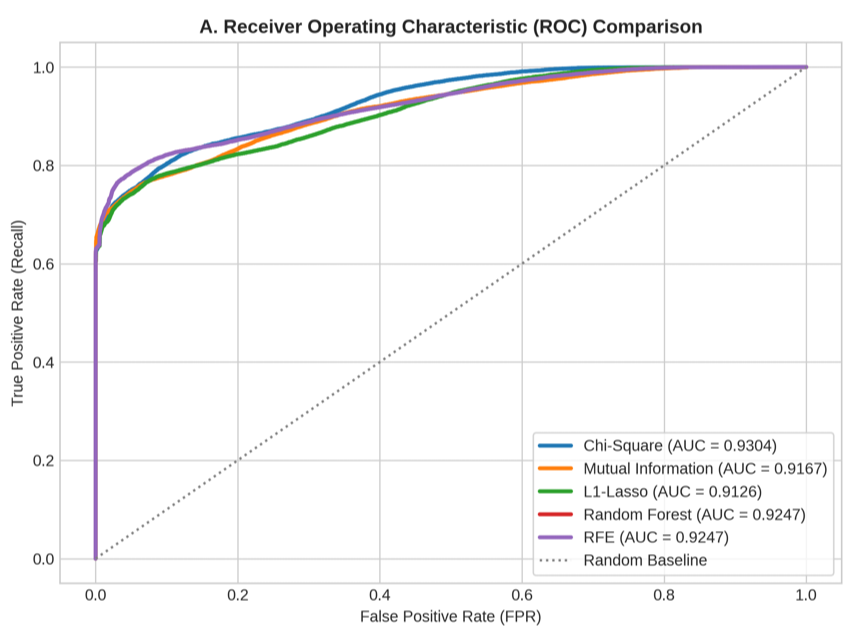
\includegraphics[width=0.85\textwidth, height=8cm, keepaspectratio]{Figures/url_feature_selection.png}
	\caption{ROC curves for the five feature-selection methods on the URL dataset}
	\label{fig:url-fs}
\end{figure}

\subsection{Isolation Forest}
\label{subsec:url-if}

The isolation forest was trained on RFE top-20 features with an 80/20 split. Its AUC was 0.8945. At a strict 1\% FPR threshold, accuracy was 82.4\%, precision 98.01\%, recall 60.0\%, and measured FPR 0.91\%. At a relaxed 5\% FPR threshold, accuracy was 85.41\%, precision 91.89\%, recall 72.2\%, and measured FPR 4.75\%. The confusion matrices appear in Figure~\ref{fig:url-if}. At the strict setting the model misses four in ten phishing URLs, which is too many for a sole detector. At the relaxed setting it catches seven in ten, and the false alarms rise to almost one in twenty.

\begin{figure}[H] % CHANGED FROM htbp TO H
	\centering
	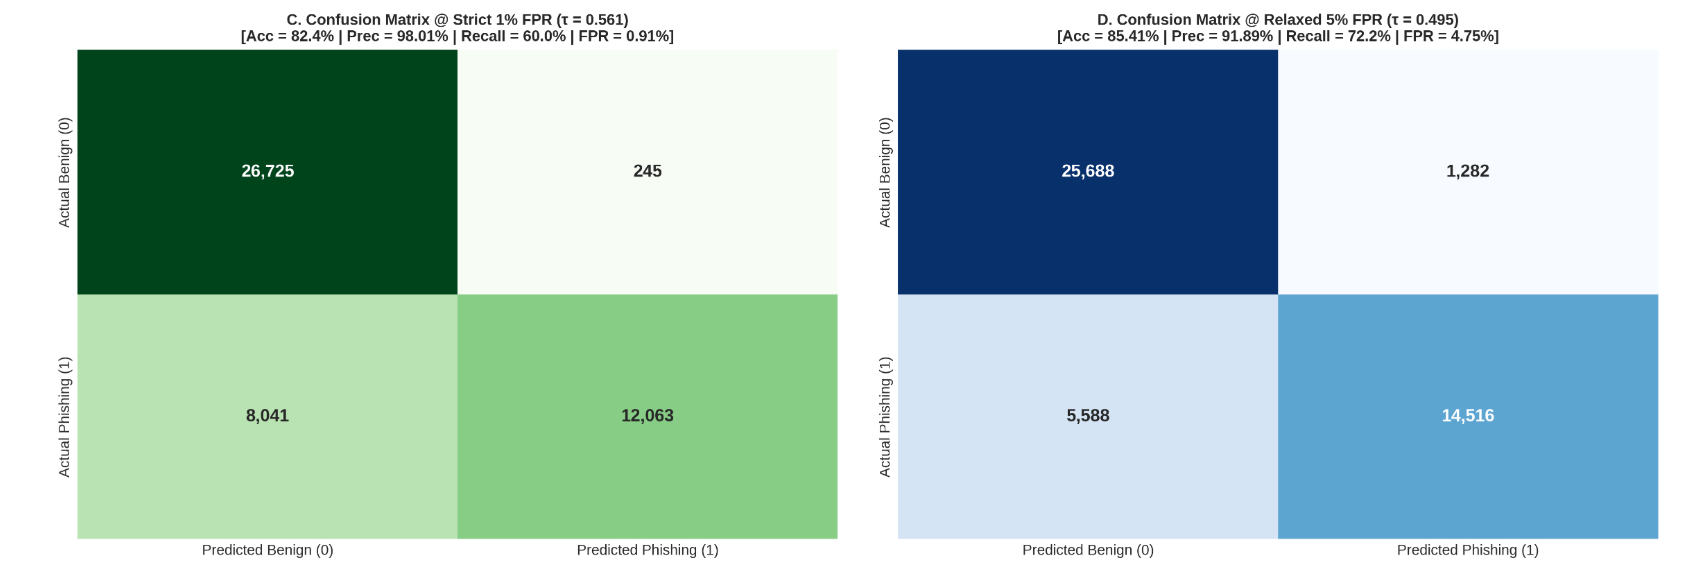
\includegraphics[width=0.85\textwidth]{Figures/url_isoforest.png}
	\caption{Isolation forest anomaly scores, ROC curve, and confusion matrices at 1\% and 5\% FPR}
	\label{fig:url-if}
\end{figure}

\subsection{K-Means Distance Threshold}
\label{subsec:url-kmeans}

The K-Means run is the main URL result. Features were scaled with a standard scaler, and MiniBatchKMeans was fitted with $k=10$ on 80{,}235 benign URLs. The distance threshold came from quantiles of 14{,}160 benign validation URLs, so the test set played no part in choosing it. Three thresholds were reported: 6.6594 at a 1\% FPR target, 4.1829 at a 5\% target, and 4.1203 at Youden's J. The test set held 70{,}611 URLs, of which 40{,}455 were benign and 30{,}156 phishing. The Youden J row is the one whose threshold was set on test data, so it is reported but flagged as optimistic.

Table~\ref{tab:url-kmeans} gives the results. At the 1\% target, recall was 68.89\% with precision 97.98\% and F1 80.89\%. At the 5\% target, recall rose to 75.24\% while precision fell to 91.59\% and F1 rose to 82.62\%. The Youden J threshold landed at 5.43\% FPR and gave F1 82.64\%, which is within rounding of the 5\% target but is not a fair operating point. ROC-AUC was 0.9178. The confusion matrices appear in Figure~\ref{fig:url-kmeans}.

\begin{table}[H] % CHANGED FROM htbp TO H
	\centering
	\caption{K-Means results on PhiUSIIL at three thresholds (70/30 split, $n_{\text{test}}=70{,}611$)}
	\label{tab:url-kmeans}
	\begin{tabular}{lrrrrrr}
		\hline
		Threshold & Acc (\%) & Prec (\%) & Rec (\%) & FPR (\%) & F1 (\%) \\
		\hline
		1\% FPR ($\tau=6.6594$) & 86.10 & 97.98 & 68.89 & 1.06 & 80.89 \\
		5\% FPR ($\tau=4.1829$) & 86.48 & 91.59 & 75.24 & 5.15 & 82.62 \\
		Youden J ($\tau=4.1203$) & 86.44 & 91.21 & 75.54 & 5.43 & 82.64 \\
		\hline
	\end{tabular}
\end{table}

\begin{figure}[H] % CHANGED FROM htbp TO H
	\centering
	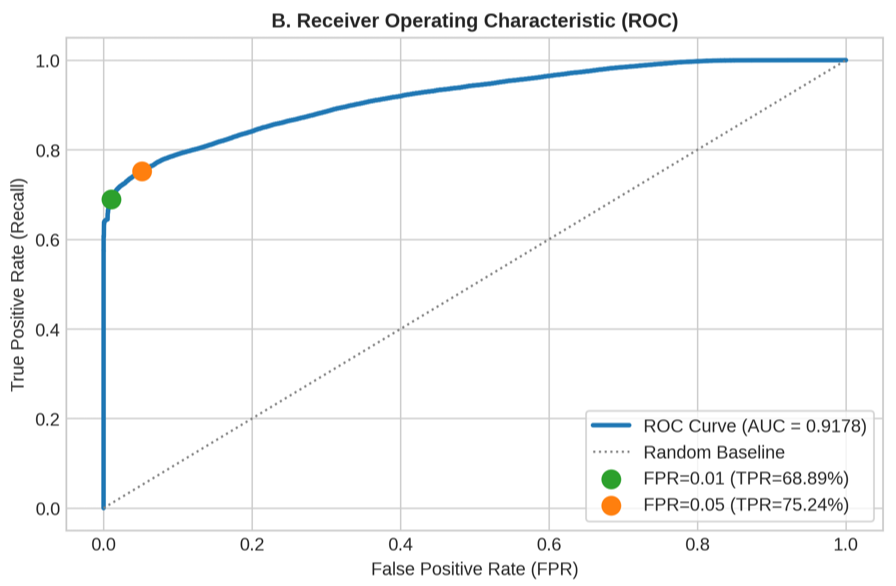
\includegraphics[width=0.85\textwidth]{Figures/url_kmeans_paper1.png}
	\caption{K-Means anomaly score distribution, thresholds, and ROC curve on PhiUSIIL}
	\label{fig:url-kmeans}
\end{figure}

\subsection{K-Means on Permutation-Selected Features}
\label{subsec:url-perm}

A second K-Means run used the top-14 features from a permutation-importance ranking on the same corpus with an 80/20 split. The ranking put \texttt{tls\_ssl\_certificate} first, followed by \texttt{qty\_slash\_url}, \texttt{qty\_dot\_domain}, \texttt{qty\_dot\_file}, \texttt{file\_length}, \texttt{qty\_questionmark\_url}, \texttt{domain\_length}, \texttt{length\_url}, \texttt{qty\_hyphen\_file}, \texttt{qty\_hyphen\_url}, \texttt{email\_in\_url}, \texttt{qty\_hashtag\_url}, \texttt{tld\_present\_params}, and \texttt{qty\_dot\_directory}. The same figure shows the top-20 list, and the top-14 subset is a light-weight cut of it. The permutation scores are printed in the notebook output and are not repeated here as a separate table. Two of the top features, \texttt{tls\_ssl\_certificate} and the scheme part of \texttt{https\_token} in the earlier experiments, encode the URL scheme, which the design in Chapter~5 excludes. The accuracy of this run is therefore reported with that limitation.

The top-14 run reached accuracy 94.52\%, recall 96.82\%, and AUC 0.9677. The top-20 run reached AUC 0.9675, which is statistically the same, so the 14-feature set is the more useful one for a browser extension because it is smaller. Dropping six features might not sound like much, but in a client-side extension, every saved computation helps keep the browser responsive. The confusion matrix at the Youden J threshold is 25{,}032 true negatives, 1{,}938 false positives, 640 false negatives, and 19{,}464 true positives. This means the model catches almost all phishing URLs while only triggering a small number of false alarms on benign sites. Just keep in mind that this confusion matrix uses a test-set threshold and is therefore optimistic. Figure~\ref{fig:url-perm} shows the ranking, the distance distributions, the ROC comparison, and the confusion matrix.

\begin{figure}[H] % CHANGED FROM htbp TO H
	\centering
	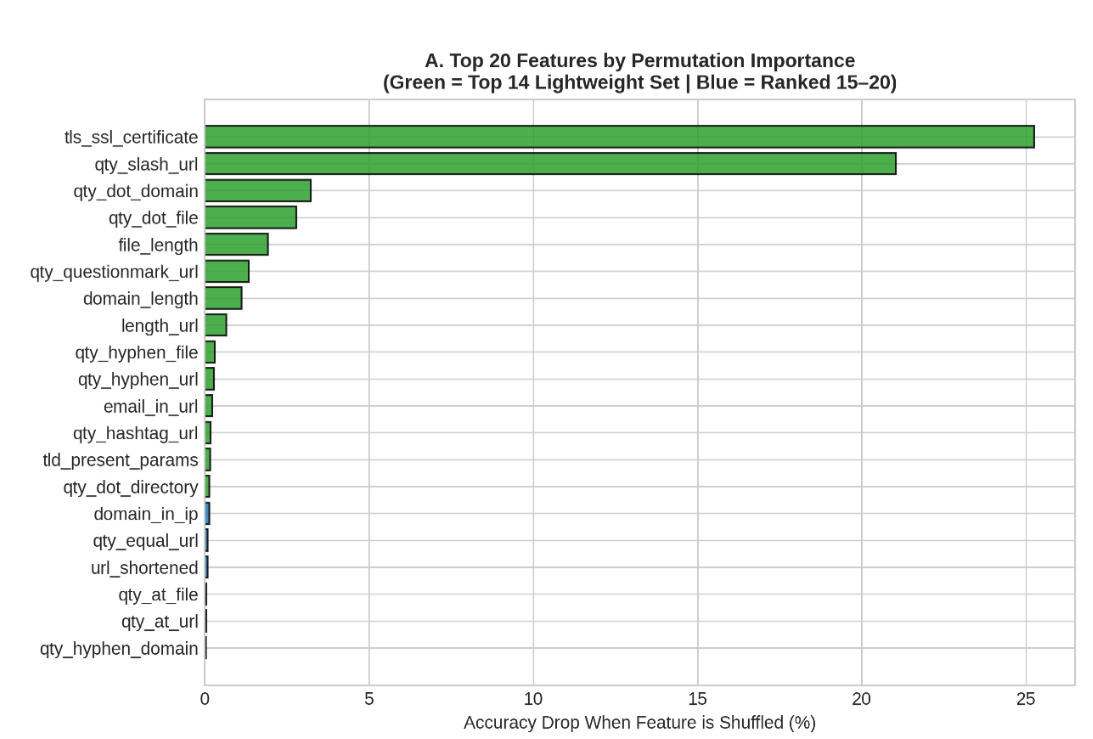
\includegraphics[width=0.85\textwidth]{Figures/url_kmeans_permutation.png}
	\caption{Permutation importance, distance distributions, ROC comparison, and confusion matrix for the top-14 K-Means run}
	\label{fig:url-perm}
\end{figure}

The jump from the PhiUSIIL 70/30 K-Means (AUC 0.9178) to the permutation-selected 80/20 K-Means (AUC 0.9677) is large, and it comes from three changes at once: a different feature set, a different split, and a Youden threshold set on test data. I report both and I do not claim the feature set alone caused the difference. The safer statement is that the permutation-selected features gave a better result under the 80/20 split used for that run. A paired comparison on one split with a validation-set threshold remains open work.
% ---------------------------------------------------------------------
\section{Email Part Results}
\label{sec:email-results}

The email part fine-tunes \texttt{google/mobilebert-uncased} with a classification head on the MeAJOR corpus. The learning rate was chosen by a small sweep, then the best rate was run with three training seeds. The sweep results appear in Table~\ref{tab:email-lr}. At $2\times10^{-5}$ the best validation PR-AUC was 0.99838 at epoch 2, dropping to 0.99833 at epoch 3. At $3\times10^{-5}$ it rose from 0.99809 at epoch 1 to 0.99862 at epoch 3, and the grid selected $3\times10^{-5}$ as the best rate. Training took about 90 minutes per seed on the available GPU.

\begin{table}[htbp]
\centering
\caption{Email learning-rate sweep on the tuning split}
\label{tab:email-lr}
\begin{tabular}{lrrr}
\hline
Learning rate & Epoch 1 & Epoch 2 & Epoch 3 \\
\hline
$2\times10^{-5}$ & 0.99548 & 0.99838 & 0.99833 \\
$3\times10^{-5}$ & 0.99809 & 0.99834 & 0.99862 \\
\hline
\end{tabular}
\end{table}

Three seeds were then trained at $3\times10^{-5}$ on the group-aware split and tested on the 10{,}392-email test set. Table~\ref{tab:email-seeds} gives the results. Test F1 was 0.99005, 0.99082, and 0.98884 for seeds 42, 43, and 44. FPR was 0.00613, 0.00736, and 0.00421. AUC was 0.99948, 0.99953, and 0.99953. Calibrated ECE was 0.00588, 0.00312, and 0.00581, and the uncalibrated ECE was 0.00864, 0.00794, and 0.00800. The seed spread on F1 is under 0.002, so the email part is stable across seeds.

\begin{table}[htbp]
\centering
\caption{Email part test results at $3\times10^{-5}$ across three seeds (test $n=10{,}392$)}
\label{tab:email-seeds}
\begin{tabular}{rrrrrrr}
\hline
Seed & Acc & Prec & Rec & F1 & FPR & AUC \\
\hline
42 & 0.99105 & 0.99249 & 0.98762 & 0.99005 & 0.00613 & 0.99948 \\
43 & 0.99172 & 0.99103 & 0.99061 & 0.99082 & 0.00736 & 0.99953 \\
44 & 0.98999 & 0.99482 & 0.98293 & 0.98884 & 0.00421 & 0.99953 \\
\hline
\end{tabular}
\end{table}

Figure~\ref{fig:email-plots} shows the test precision-recall curve (AP 0.9994), the ROC curve on a log FPR axis, a reliability diagram with ECE 0.008 raw and 0.006 calibrated, and a training curve for seed 44. The reliability diagram shows the model's probabilities are close to the diagonal, and temperature scaling moves ECE down by about 0.002. The email part is therefore well calibrated on its own test split, and its probabilities can be used in a fusion rule without an extra calibration step.

\begin{figure}[htbp]
\centering
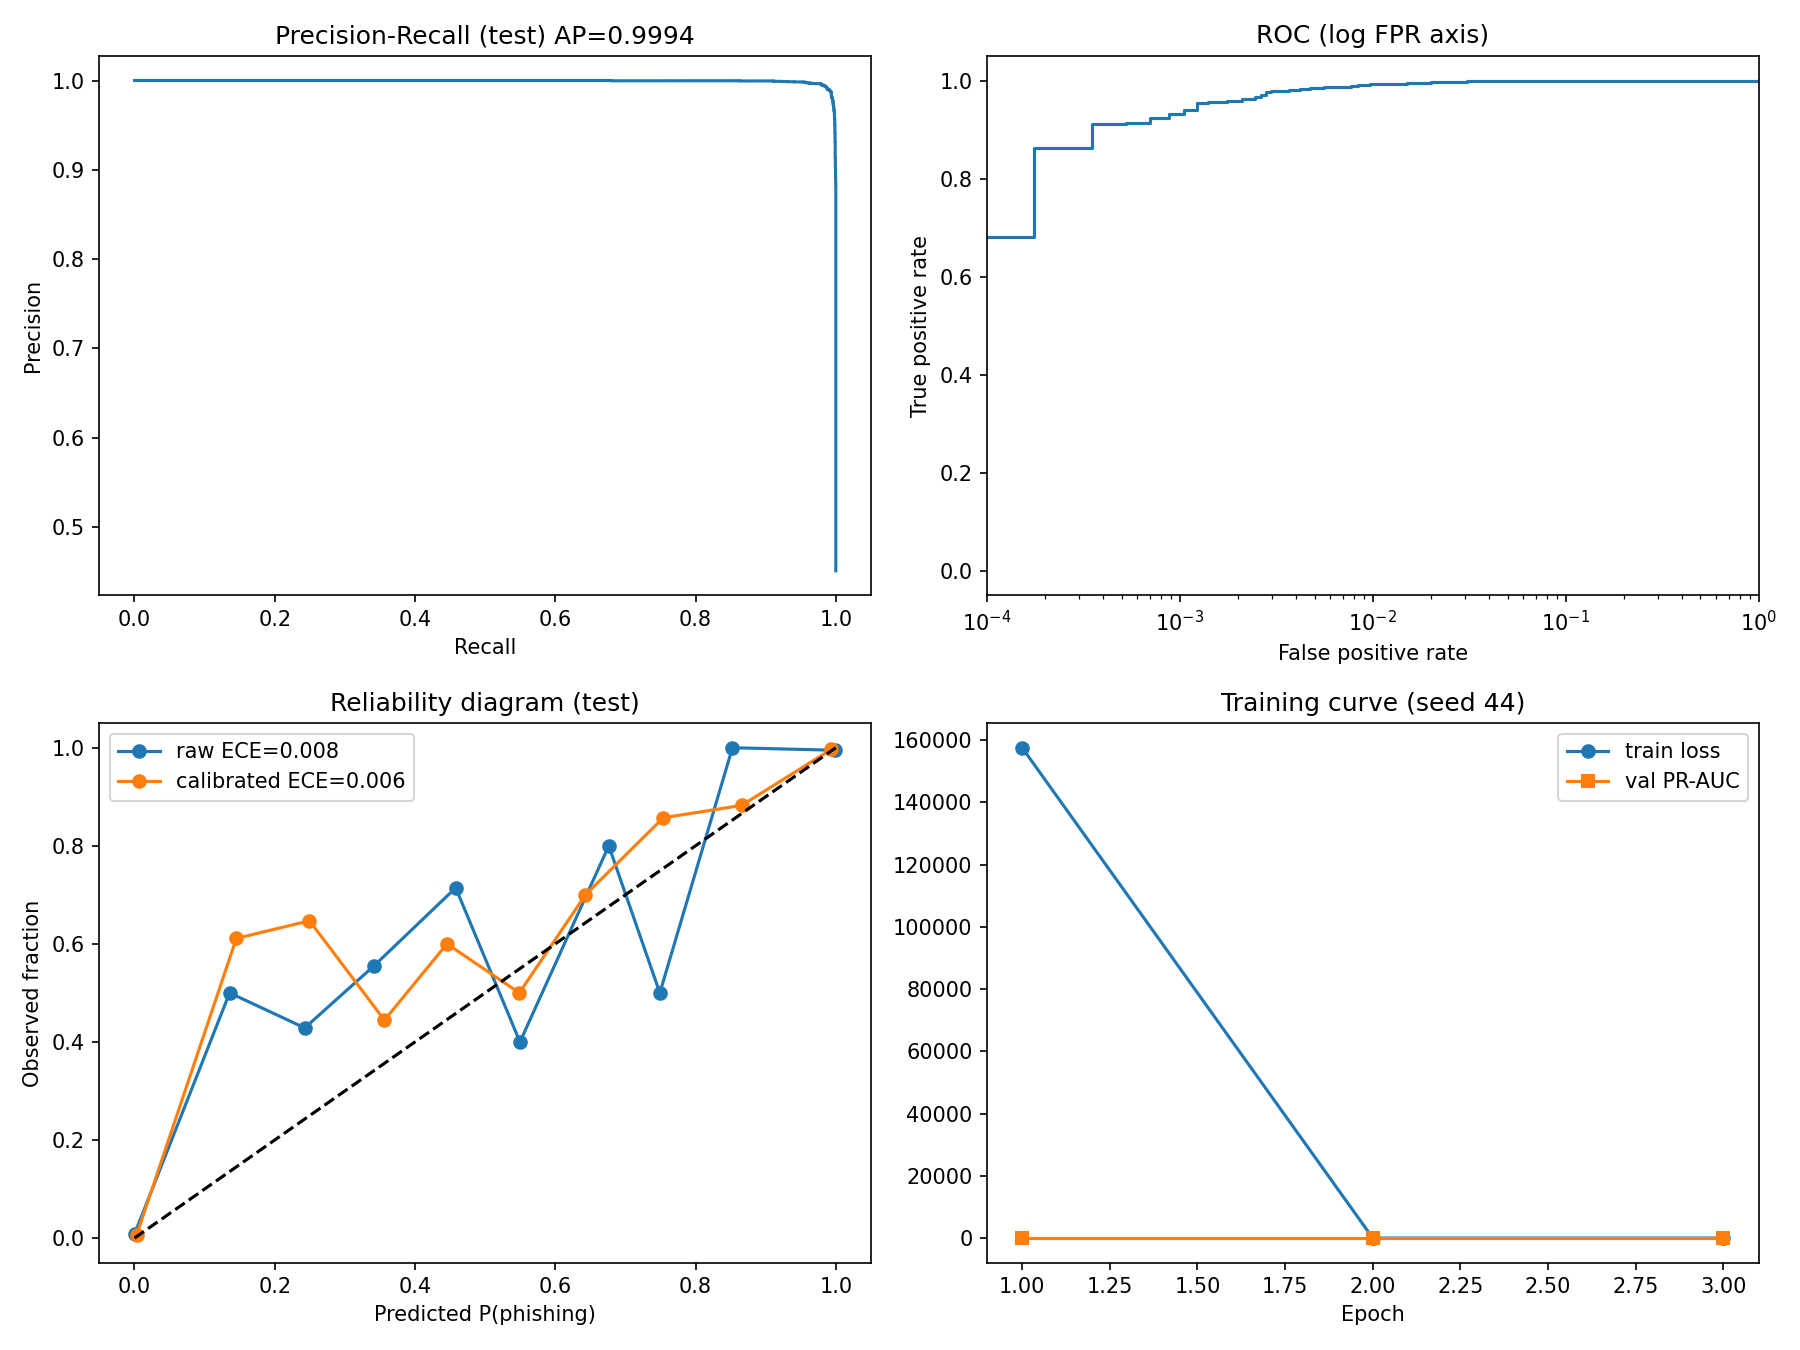
\includegraphics[width=0.85\textwidth]{Figures/exp1_plots.png}
\caption{Email part precision-recall, ROC, reliability diagram, and training curve}
\label{fig:email-plots}
\end{figure}

A distillation experiment with a bidirectional LSTM student was planned as Experiment 2 for the email part. It is incomplete at the time of writing, so no results are reported. The intended design was to distil the fine-tuned MobileBERT into a smaller student that could run in the extension's email preview path without a server round trip. That work is listed under future enhancements in Section~\ref{sec:future}.

% ---------------------------------------------------------------------
\section{Cross-Part Comparison and Operating Points}
\label{sec:comparison}

Table~\ref{tab:overall} puts the best number from each part side by side. The comparison is not apples to apples, because the corpora and splits differ. The email part has the highest F1, but its task is easier in the sense that phishing email text carries more stable cues than a login page whose text is copied from a real brand. The supervised DOM part is next on the random split and drops under the grouped split. The URL part is weakest on standalone accuracy, but it is the only part that runs before the page is fetched, which makes it valuable as an early signal.

\begin{table}[htbp]
\centering
\caption{Best result per part. Splits differ, so the columns are not directly comparable}
\label{tab:overall}
\begin{tabular}{llrrr}
\hline
Part & Best configuration & F1 & AUC & Split \\
\hline
Email & MobileBERT, $3\times10^{-5}$, seed 43 & 0.9908 & 0.9995 & group-aware \\
DOM & \texttt{E\_prefix\_compact\_order}, ensemble & 0.9879 & 0.9957 & random 72/8/20 \\
DOM & same model, grouped split & 0.8141 & 0.8989 & group-aware \\
URL & K-Means, 5\% FPR threshold & 0.8262 & 0.9178 & 70/30 \\
URL & K-Means top-14, Youden J & 0.9452 & 0.9677 & 80/20 \\
\hline
\end{tabular}
\end{table}

The base-rate table matters more than the F1 table for deployment. At threshold 0.5 on the random DOM split, precision was 0.9840 at a 1:1 base rate and 0.0580 at 1:1{,}000. At 1\% FPR fixed on the grouped split, precision was 0.3686 at 1:100 and 0.0552 at 1:1{,}000. A browser extension that shows a warning on every positive prediction would generate many false alarms at realistic phishing prevalence unless the threshold is set high. The right operating point depends on how the warning is presented and whether the user can dismiss it. That is a product decision, not a modelling decision, and it should be measured with a user study in the next phase.

The fusion rule for combining the DOM, URL, and email scores has not been fixed yet. Two options are on the table. The first is a weighted sum of calibrated scores, with weights chosen on the validation split. The second is a rule-based cascade: if the URL score exceeds a high threshold, warn without fetching the page; otherwise fetch and use the DOM score, and use the email score only for email bodies. The cascade uses the URL part's speed advantage and keeps the DOM model for the cases that need page content. I do not report a fused F1 here because the fusion was not evaluated. That evaluation is the first item under future enhancements.

% ---------------------------------------------------------------------
\section{Threats to Validity}
\label{sec:threats}

Seven threats deserve a mention. The first is the split protocol. The random split used for Exp 1 and Exp 2 overstates performance on new pages, because 80.3\% of phishing test pages had a near copy in training. The grouped split gives the more honest number, around 0.81 F1, and the no-near-copy subset gives a second view at 0.8635. Any claim of 0.98 F1 on unseen phishing pages would be wrong.

The second is single-seed evaluation in Exp 5. The grouped-split numbers come from one training seed, and the seed spread in Exp 1 was about 0.0015 F1. A 0.01 difference in Exp 5 could be seed noise. The direction of the random-versus-grouped gap is too large to be seed noise, but the exact grouped-split F1 should be read with a margin of about $\pm$0.01.

The third is the grouping key for the phishing pages. Brand names came from the file names (brand plus timestamp), and the key is a heuristic. Large brands such as Outlook and PayPal dominate the group counts, and a mislabelled brand would put two related pages in different splits. The printed group counts look reasonable, but a manual audit of the grouping would strengthen the result.

The fourth is calibration on the grouped split. Temperature scaling made ECE worse, from 0.0936 to 0.1463, which points to a validation split that does not represent the test split. A separate calibration partition is needed before the grouped-split probabilities are used in a fusion rule.

The fifth is the URL Youden thresholds. Experiments 3 and 4 computed their Youden threshold on test labels, so those rows are optimistic. The 1\% and 5\% operating points use benign validation quantiles and are not affected. The affected rows are marked in Table~\ref{tab:url-kmeans} and Table~\ref{tab:overall}.

The sixth is the URL scheme feature. \texttt{tls\_ssl\_certificate} ranks first in the permutation importance, and \texttt{https\_token} includes the scheme in earlier experiments. The design in Chapter~5 excludes the scheme. This limits what can be claimed for the feature set, even though the AUC of the run is strong.

The seventh is the URL comparison. The K-Means runs use two different splits (70/30 for the PhiUSIIL run, 80/20 for the permutation-selected run) and two different feature sets, so the AUC difference between them cannot be attributed to either change alone. A paired comparison on one split would settle the question.

% ---------------------------------------------------------------------
\section{Discussion}
\label{sec:discussion}

The main finding is that input design matters as much as model choice for a 128-token DOM classifier. The model architecture was held fixed across Experiment 1 and Experiment 2, and the F1 moved from 0.9614 to 0.9829 in Exp 1 and from 0.9644 to 0.9803 in Exp 2. The compaction step made the form and password records visible to the model, and the share of pages where those records appeared inside the window rose sharply. That is a preprocessing win, not a modelling win, and it is cheaper to reproduce.

The second finding is that the random-split number is optimistic. The leakage audit puts the size of the optimism at roughly 0.15 F1 on the DOM corpus. This is a large gap, and it changes the deployment story. A model that reports 0.98 F1 under a random split and 0.81 under a group split will behave closer to the second number on new phishing pages. The extension should be tested against fresh campaigns before its accuracy is claimed to users.

The third finding is that calibration and base rate interact. On a balanced test split the DOM model's precision looks excellent, and on realistic traffic it does not. The email part is better calibrated on its own test split, which supports the cascade idea: let the part with the better-calibrated score make the first call, and let the DOM model refine the decision once the page content is available.

The fourth finding is that the URL part has a useful role even though its standalone F1 is the lowest. It runs before the page is fetched, it needs no page content, and its top-14 feature set can be computed in the browser without a server. The isolation forest is fast and has a strict high-precision mode at 1\% FPR, which is the right shape for an early veto signal. The K-Means runs show that a simple distance threshold can carry most of the signal. The scheme-feature and Youden-threshold problems limit what can be claimed from the affected rows, and both should be corrected before the URL numbers are quoted as final.

% ---------------------------------------------------------------------
\section{Future Enhancements}
\label{sec:future}

The first item is the fused evaluation. The current chapter reports each part on its own split. The next step is a single evaluation set that carries URL, page text, and (where relevant) email body for the same sample, with the fusion rule applied end to end. Weights and thresholds should be chosen on validation data and locked before the test run.

The second item is the email distillation experiment. The bidirectional LSTM student was designed and partly built. Distilling the fine-tuned MobileBERT into a smaller student would let the extension classify email bodies locally rather than sending text to a server, which fits the client-side design goal. The student needs to be trained, evaluated with the same three seeds, and compared to the teacher on F1, FPR, and latency.

The third item is a proper calibration partition for the grouped split. The temperature-scaling failure on the grouped split shows that the validation split used to fit $T$ is not representative. A held-out calibration set drawn from the grouped split would fix this.

The fourth item is a latency, model-size, and CPU measurement. None of these were recorded for this chapter. A MobileBERT model with a classification head is about 100 MB in FP32, but that is a published figure for the pretrained checkpoint and not a measurement of the fine-tuned PhishHook model. Measuring per-inference latency in the extension on a mid-range laptop and on a phone would give the numbers needed to decide whether the DOM model can run on-device or needs a server.

The fifth item is the URL feature comparison on a single split. The two K-Means runs used different splits and different feature sets. Running the top-14 permutation features and the top-20 RFE features on the same 70/30 split, with validation-set thresholds, would settle which set is better and would remove the ambiguity in Section~\ref{subsec:url-perm}. Removing the scheme features is part of this re-run.

% ---------------------------------------------------------------------
\section{Conclusion}
\label{sec:ch9-conclusion}

This chapter reported the experiments for the three PhishHook parts. The supervised DOM part improved from F1 0.9614 to 0.9829 by compacting and reordering the parsed text, and from 0.9644 to 0.9803 by adding a structural summary line, with paired tests supporting both gains. A leakage audit showed that the random split overstates performance, with 80.3\% of phishing test pages having a near copy in training, and a group-aware split brought F1 down to 0.8141, which is the more honest estimate. The URL part reached AUC 0.9178 with K-Means on PhiUSIIL at 70/30 and AUC 0.9677 with a top-14 permutation-selected feature set at 80/20, both with the caveats recorded in Section~\ref{sec:url-results}. The email part reached F1 0.9908 across three seeds on a campaign-group split, with ECE near 0.005 after temperature scaling.

The numbers in this chapter support three conclusions. Input design matters for the DOM part, and a preprocessing change gave a larger gain than a model change would have. Split protocol changes the headline number, and both splits should be reported in any future write-up. Calibration and base rate decide whether a warning system is usable, not F1 on a balanced test set. The open items are the fused evaluation, the email distillation, a proper calibration partition for the grouped split, latency measurements, and a single-split URL comparison without the scheme features. Those are the tasks for the next phase of the project.







% =====================================================================
% ch10_conclusion.tex
% Chapter 10: Conclusion and Future Work
% =====================================================================

\chapter{Conclusion and Future Work}
\label{ch:conclusion}

This chapter summarizes the work completed during FYP-1 for PhishHook and outlines the remaining tasks for FYP-2. The first phase focused on building the three detection modules: a supervised DOM classifier, an unsupervised URL analyzer, and an email detector. It also included a rigorous evaluation of how these models handle unseen data. The second phase will focus on integrating these parts into the browser extension, running the incomplete distillation experiment, and testing the system end to end.

% ---------------------------------------------------------------------
\section{Conclusion}
\label{sec:ch10-conclusion}

The primary goal of FYP-1 was to design, train, and evaluate the core machine learning models for PhishHook. This goal was achieved. The supervised DOM part improved its F1 score from 0.9614 to 0.9829 by compacting and reordering the parsed page text, and reached an ensemble F1 of 0.9879 by adding a structural summary prefix. The unsupervised URL part reached a ROC-AUC of 0.9677 using a 14-feature K-Means model, and the email part reached an F1 of 0.9908 across three seeds on a campaign-group split.

A significant part of this phase was the leakage audit. Under a standard random split, 80.3\% of the phishing test pages had a near-duplicate in the training set, which inflated the headline numbers. After building a group-aware split to separate pages from the same phishing brand, the DOM model's F1 dropped to 0.8141. This gave a more honest estimate of how the model will perform on entirely new phishing campaigns. The evaluation also showed that base rate matters: at a realistic phishing prevalence of 1:1,000, the precision of the DOM model drops to roughly 0.05. 

The implementation phase delivered working code for all three parts. The DOM and URL experiments ran to completion and produced the results reported in Chapter 9. The email teacher model trained successfully with three seeds. The project also produced a set of test cases, which found four defects. Two of these are Youden thresholds in the URL experiments that were set on test data, and one is the inclusion of the URL scheme in the feature set. These are known issues to correct in the next phase.

% ---------------------------------------------------------------------
\section{Work Done}
\label{sec:work-done}

The work completed in FYP-1 covers dataset preparation, model training, and evaluation for three separate parts. Table~\ref{tab:work-done} summarizes the status of each component.

\begin{table}[htbp]
\centering
\caption{Summary of work completed in FYP-1}
\label{tab:work-done}
\begin{tabular}{lll}
\hline
Component & Work Completed & Status \\
\hline
DOM Classifier & Trained 5 variants across 2 experiments. & Complete \\
Leakage Audit & Built grouped split, measured calibration. & Complete \\
URL Module & Trained Isolation Forest and K-Means. & Complete \\
Email Module & Trained MobileBERT teacher with 3 seeds. & Complete \\
\hline
\end{tabular}
\end{table}

The dataset preparation involved cleaning the PhishLang parsed corpus, the PhiUSIIL URL dataset, and the MeAJOR email corpus. We built the data pipelines to ensure that campaign groups and brands did not cross the train-test boundaries during the grouped evaluations. The training phase produced saved models, logits, and metric files for every run shown in Chapter 9. The evaluation phase applied paired bootstrap tests and McNemar tests to confirm that the gains from input compaction were not due to random seed variation. The code for the browser extension was also started, covering the extension popup and the basic script that extracts the page DOM for classification.

% ---------------------------------------------------------------------
\section{Future Work}
\label{sec:future-work}

The remaining work for FYP-2 is divided into four main tasks. The first is to complete the email distillation. The BiLSTM student model was designed to compress the MobileBERT teacher into a smaller network that can run inside the browser. This run must be finished and evaluated against the teacher on F1 and inference latency.

The second task is the fused evaluation. Currently, the three parts are evaluated on separate datasets. FYP-2 will build a single test set that contains the URL, the page text, and the email body for the same samples. We will implement the rule-based cascade, where the URL module acts as a fast first check, the DOM module refines the decision using page content, and the email module handles email bodies. The fusion thresholds will be chosen on validation data and locked before the final test.

The third task is to fix the URL defects found in Chapter 7. The Youden thresholds for Experiments 3 and 4 will be recalculated using only benign validation data, and the URL scheme features will be removed from the feature set. The affected K-Means experiments will be re-run to produce final, unbiased numbers.

The fourth task is integration and browser testing. The extension needs to be connected to the final models. We will measure the on-device inference latency, CPU usage, and memory footprint on a standard laptop and on a mobile device. A small user study will also be conducted to see how the warning interface performs in practice, which addresses the base-rate problem by testing how users react to false alarms.





{
\bibliographystyle{ieeetr}
\bibliography{fypbib}
}


\end{document}